\documentclass[]{article}
\usepackage{lmodern}
\usepackage{amssymb,amsmath}
\usepackage{ifxetex,ifluatex}
\usepackage{fixltx2e} % provides \textsubscript
\ifnum 0\ifxetex 1\fi\ifluatex 1\fi=0 % if pdftex
  \usepackage[T1]{fontenc}
  \usepackage[utf8]{inputenc}
\else % if luatex or xelatex
  \ifxetex
    \usepackage{mathspec}
  \else
    \usepackage{fontspec}
  \fi
  \defaultfontfeatures{Ligatures=TeX,Scale=MatchLowercase}
\fi
% use upquote if available, for straight quotes in verbatim environments
\IfFileExists{upquote.sty}{\usepackage{upquote}}{}
% use microtype if available
\IfFileExists{microtype.sty}{%
\usepackage{microtype}
\UseMicrotypeSet[protrusion]{basicmath} % disable protrusion for tt fonts
}{}
\usepackage[margin=1in]{geometry}
\usepackage{hyperref}
\hypersetup{unicode=true,
            pdftitle={Background},
            pdfauthor={Sean Davis},
            pdfborder={0 0 0},
            breaklinks=true}
\urlstyle{same}  % don't use monospace font for urls
\usepackage{color}
\usepackage{fancyvrb}
\newcommand{\VerbBar}{|}
\newcommand{\VERB}{\Verb[commandchars=\\\{\}]}
\DefineVerbatimEnvironment{Highlighting}{Verbatim}{commandchars=\\\{\}}
% Add ',fontsize=\small' for more characters per line
\usepackage{framed}
\definecolor{shadecolor}{RGB}{248,248,248}
\newenvironment{Shaded}{\begin{snugshade}}{\end{snugshade}}
\newcommand{\KeywordTok}[1]{\textcolor[rgb]{0.13,0.29,0.53}{\textbf{#1}}}
\newcommand{\DataTypeTok}[1]{\textcolor[rgb]{0.13,0.29,0.53}{#1}}
\newcommand{\DecValTok}[1]{\textcolor[rgb]{0.00,0.00,0.81}{#1}}
\newcommand{\BaseNTok}[1]{\textcolor[rgb]{0.00,0.00,0.81}{#1}}
\newcommand{\FloatTok}[1]{\textcolor[rgb]{0.00,0.00,0.81}{#1}}
\newcommand{\ConstantTok}[1]{\textcolor[rgb]{0.00,0.00,0.00}{#1}}
\newcommand{\CharTok}[1]{\textcolor[rgb]{0.31,0.60,0.02}{#1}}
\newcommand{\SpecialCharTok}[1]{\textcolor[rgb]{0.00,0.00,0.00}{#1}}
\newcommand{\StringTok}[1]{\textcolor[rgb]{0.31,0.60,0.02}{#1}}
\newcommand{\VerbatimStringTok}[1]{\textcolor[rgb]{0.31,0.60,0.02}{#1}}
\newcommand{\SpecialStringTok}[1]{\textcolor[rgb]{0.31,0.60,0.02}{#1}}
\newcommand{\ImportTok}[1]{#1}
\newcommand{\CommentTok}[1]{\textcolor[rgb]{0.56,0.35,0.01}{\textit{#1}}}
\newcommand{\DocumentationTok}[1]{\textcolor[rgb]{0.56,0.35,0.01}{\textbf{\textit{#1}}}}
\newcommand{\AnnotationTok}[1]{\textcolor[rgb]{0.56,0.35,0.01}{\textbf{\textit{#1}}}}
\newcommand{\CommentVarTok}[1]{\textcolor[rgb]{0.56,0.35,0.01}{\textbf{\textit{#1}}}}
\newcommand{\OtherTok}[1]{\textcolor[rgb]{0.56,0.35,0.01}{#1}}
\newcommand{\FunctionTok}[1]{\textcolor[rgb]{0.00,0.00,0.00}{#1}}
\newcommand{\VariableTok}[1]{\textcolor[rgb]{0.00,0.00,0.00}{#1}}
\newcommand{\ControlFlowTok}[1]{\textcolor[rgb]{0.13,0.29,0.53}{\textbf{#1}}}
\newcommand{\OperatorTok}[1]{\textcolor[rgb]{0.81,0.36,0.00}{\textbf{#1}}}
\newcommand{\BuiltInTok}[1]{#1}
\newcommand{\ExtensionTok}[1]{#1}
\newcommand{\PreprocessorTok}[1]{\textcolor[rgb]{0.56,0.35,0.01}{\textit{#1}}}
\newcommand{\AttributeTok}[1]{\textcolor[rgb]{0.77,0.63,0.00}{#1}}
\newcommand{\RegionMarkerTok}[1]{#1}
\newcommand{\InformationTok}[1]{\textcolor[rgb]{0.56,0.35,0.01}{\textbf{\textit{#1}}}}
\newcommand{\WarningTok}[1]{\textcolor[rgb]{0.56,0.35,0.01}{\textbf{\textit{#1}}}}
\newcommand{\AlertTok}[1]{\textcolor[rgb]{0.94,0.16,0.16}{#1}}
\newcommand{\ErrorTok}[1]{\textcolor[rgb]{0.64,0.00,0.00}{\textbf{#1}}}
\newcommand{\NormalTok}[1]{#1}
\usepackage{longtable,booktabs}
\usepackage{graphicx,grffile}
\makeatletter
\def\maxwidth{\ifdim\Gin@nat@width>\linewidth\linewidth\else\Gin@nat@width\fi}
\def\maxheight{\ifdim\Gin@nat@height>\textheight\textheight\else\Gin@nat@height\fi}
\makeatother
% Scale images if necessary, so that they will not overflow the page
% margins by default, and it is still possible to overwrite the defaults
% using explicit options in \includegraphics[width, height, ...]{}
\setkeys{Gin}{width=\maxwidth,height=\maxheight,keepaspectratio}
\IfFileExists{parskip.sty}{%
\usepackage{parskip}
}{% else
\setlength{\parindent}{0pt}
\setlength{\parskip}{6pt plus 2pt minus 1pt}
}
\setlength{\emergencystretch}{3em}  % prevent overfull lines
\providecommand{\tightlist}{%
  \setlength{\itemsep}{0pt}\setlength{\parskip}{0pt}}
\setcounter{secnumdepth}{5}
% Redefines (sub)paragraphs to behave more like sections
\ifx\paragraph\undefined\else
\let\oldparagraph\paragraph
\renewcommand{\paragraph}[1]{\oldparagraph{#1}\mbox{}}
\fi
\ifx\subparagraph\undefined\else
\let\oldsubparagraph\subparagraph
\renewcommand{\subparagraph}[1]{\oldsubparagraph{#1}\mbox{}}
\fi

%%% Use protect on footnotes to avoid problems with footnotes in titles
\let\rmarkdownfootnote\footnote%
\def\footnote{\protect\rmarkdownfootnote}

%%% Change title format to be more compact
\usepackage{titling}

% Create subtitle command for use in maketitle
\newcommand{\subtitle}[1]{
  \posttitle{
    \begin{center}\large#1\end{center}
    }
}

\setlength{\droptitle}{-2em}
  \title{Background}
  \pretitle{\vspace{\droptitle}\centering\huge}
  \posttitle{\par}
  \author{Sean Davis}
  \preauthor{\centering\large\emph}
  \postauthor{\par}
  \predate{\centering\large\emph}
  \postdate{\par}
  \date{6/29/2017}


\usepackage{amsthm}
\newtheorem{theorem}{Theorem}[section]
\newtheorem{lemma}{Lemma}[section]
\theoremstyle{definition}
\newtheorem{definition}{Definition}[section]
\newtheorem{corollary}{Corollary}[section]
\newtheorem{proposition}{Proposition}[section]
\theoremstyle{definition}
\newtheorem{example}{Example}[section]
\theoremstyle{remark}
\newtheorem*{remark}{Remark}
\begin{document}
\maketitle

{
\setcounter{tocdepth}{2}
\tableofcontents
}
\section{Why R?}\label{why-r}

\subsection{What is R?}\label{what-is-r}

R is a number of things, simultaneously. Depending on who is being
asked, R is:

\begin{itemize}
\tightlist
\item
  A software package
\item
  A programming language
\item
  A toolkit for developing statistical and analytical tools
\item
  An extensive library of statistical and mathematical software and
  algorithms
\item
  A scripting language
\item
  much, much more
\end{itemize}

\subsection{Why use R?}\label{why-use-r}

\begin{itemize}
\tightlist
\item
  R is cross-platform and runs on Windows, Mac, and Linux (as well as
  more obscure systems).
\item
  R provides a vast number of useful statistical tools, many of which
  have been painstakingly tested.
\item
  R produces publication-quality graphics in a variety of formats.
\item
  R plays well with FORTRAN, C, and scripts in many languages.
\item
  R scales, making it useful for small and large projects. It is NOT
  Excel.
\item
  R does not have a meaningfully useful graphical user interface (GUI).
\end{itemize}

I can develop code for analysis on my Mac laptop. I can then install the
\emph{same} code on our 20k core cluster and run it in parallel on 100
samples, monitor the process, and then update a database (for example)
with R when complete.

\subsection{Why not use R?}\label{why-not-use-r}

\begin{itemize}
\tightlist
\item
  R cannot do everything.
\item
  R is not always the ``best'' tool for the job.
\item
  R will \emph{not} hold your hand. Often, it will \emph{slap} your hand
  instead.
\item
  The documentation can be opaque (but there is documentation).
\item
  R can drive you crazy (on a good day) or age you prematurely (on a bad
  one).
\item
  Finding the right package to do the job you want to do can be
  challenging; worse, some contributed packages are unreliable.{]}\{\}
\item
  R does not have a meaningfully useful graphical user interface (GUI).
\end{itemize}

\subsection{R License and the Open Source
Ideal}\label{r-license-and-the-open-source-ideal}

R is free (yes, totally free!) and distributed under GNU license. In
particular, this license allows one to:

\begin{itemize}
\tightlist
\item
  Download the source code
\item
  Modify the source code to your heart's content
\item
  Distribute the modified source code and even charge money for it, but
  you must distribute the modified source code under the original GNU
  license{]}\{\}
\end{itemize}

This license means that R will always be available, will always be open
source, and can grow organically without constraint.

\section{R Mechanics}\label{r-mechanics}

\subsection{Installing R}\label{installing-r}

The home page for R is called the Comprehensive R Archive Network
(CRAN). The \href{http://cran.r-project.or}{website} is not pretty (see
figure \ref{fig:cranscreenshot}), but it has quite a bit of information
on it. It is not the best place to find help on R, although it is one of
the best places to get R-related software, tools, and updates.

\begin{Shaded}
\begin{Highlighting}[]
\NormalTok{knitr}\OperatorTok{::}\KeywordTok{include_graphics}\NormalTok{(}\StringTok{'images/CRAN-screenshot.png'}\NormalTok{)}
\end{Highlighting}
\end{Shaded}

\begin{figure}
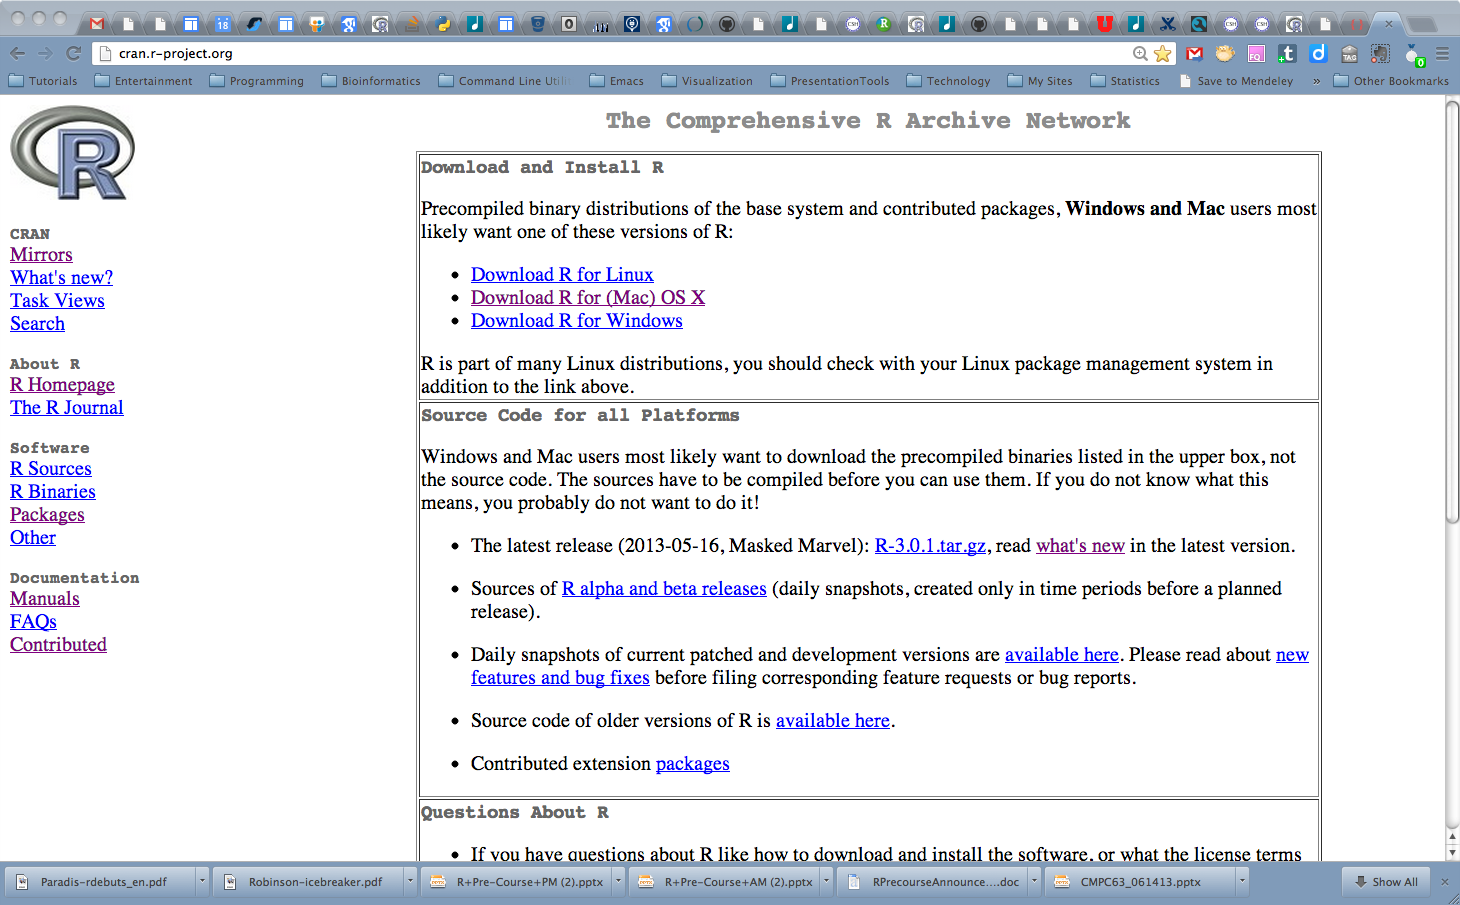
\includegraphics[width=20.28in]{images/CRAN-screenshot} \caption{The Comprehensive R Archive Network (CRAN) website}\label{fig:cranscreenshot}
\end{figure}

Detailed installation instructions are readily available, but here are
abbreviated instructions for convenience.

\subsubsection{Windows}\label{windows}

NOTE: See \href{https://cran.r-project.org/bin/windows/}{Windows
installation instructions} for more detail. Install \emph{R} and
\emph{RStudio} as regular users.

To install \emph{R}, visit the
\href{https://cran.r-project.org/bin/windows/base/}{Windows base}
distribution page. Click on the \texttt{Download\ R-3.4.0\ for\ Windows}
link (or use the latest version available). Click on the installer and
make the default selection for each option.

To install \emph{RStudio}, visit the
\href{https://www.rstudio.com/products/rstudio/download/}{RStudio
download} page. Click on the current RStudio release for Windows link.
Click on the installer and follow default instructions.

\subsubsection{Mac}\label{mac}

NOTE: See \href{https://cran.r-project.org/bin/macosx/}{R for Mac OS X}
for more detail.

To install \emph{R}, visit the
\href{https://cran.r-project.org/bin/macosx/}{R for Mac OS X}. Click on
the the \texttt{R-3.4.0.pkg} link (or use the latest version available).
Click on the installer and follow default instructions.

To install \emph{RStudio}, visit the
\href{https://www.rstudio.com/products/rstudio/download/}{RStudio
download} page. Click on the current RStudio release for Windows link.
Click on the installer and follow default instructions.

\subsubsection{Linux}\label{linux}

NOTE: See
\href{https://cran.r-project.org/bin/linux/}{distribution-specific
instructions} for additional detail.

On debian-based systems, the easiest way to install \emph{R} is through
a package manager manager, run under an administrator account. On Linux
one usually needs to install \emph{R} packages from source, and \emph{R}
package source often contains C, C++, or Fortran code requiring a
compiler and \texttt{-dev} versions of various system libraries. It is
therefore convenient to install the \texttt{-dev} version of R.

\begin{verbatim}
sudo apt-get install r-base r-base-dev
\end{verbatim}

When installing source packages, it may be necessary to have access to
the \texttt{-dev} version of various system libraries. Many of these are
installed as dependencies of \texttt{r-base-dev}; other common examples
include the xml and curl libraries

\begin{verbatim}
sudo apt-get install libxml2-dev
sudo apt-get install libcurl-dev
\end{verbatim}

Note in particular the use specification of libraries (the \texttt{lib}
prefix) and the use of the \texttt{-dev} version.

To install \emph{RStudio}, visit the
\href{https://www.rstudio.com/products/rstudio/download/}{RStudio
download} page. Download the appropriate archive for your OS. On Ubuntu,
install the \texttt{.deb} installer with

\begin{verbatim}
sudo dpkg -i rstudio-1.0.136-amd64.deb
\end{verbatim}

\subsection{Starting R}\label{starting-r}

How to start R depends a bit on the operating system (Mac, Windows,
Linux) and interface. In this course, we will largely be using an
Integrated Development Environment (IDE) called \emph{RStudio}, but
there is nothing to prohibit using R at the command line or in some
other interface (and there are a few). A screenshot of the interface is
shown in figure \ref{fig:rstudiointerface}.

\begin{figure}
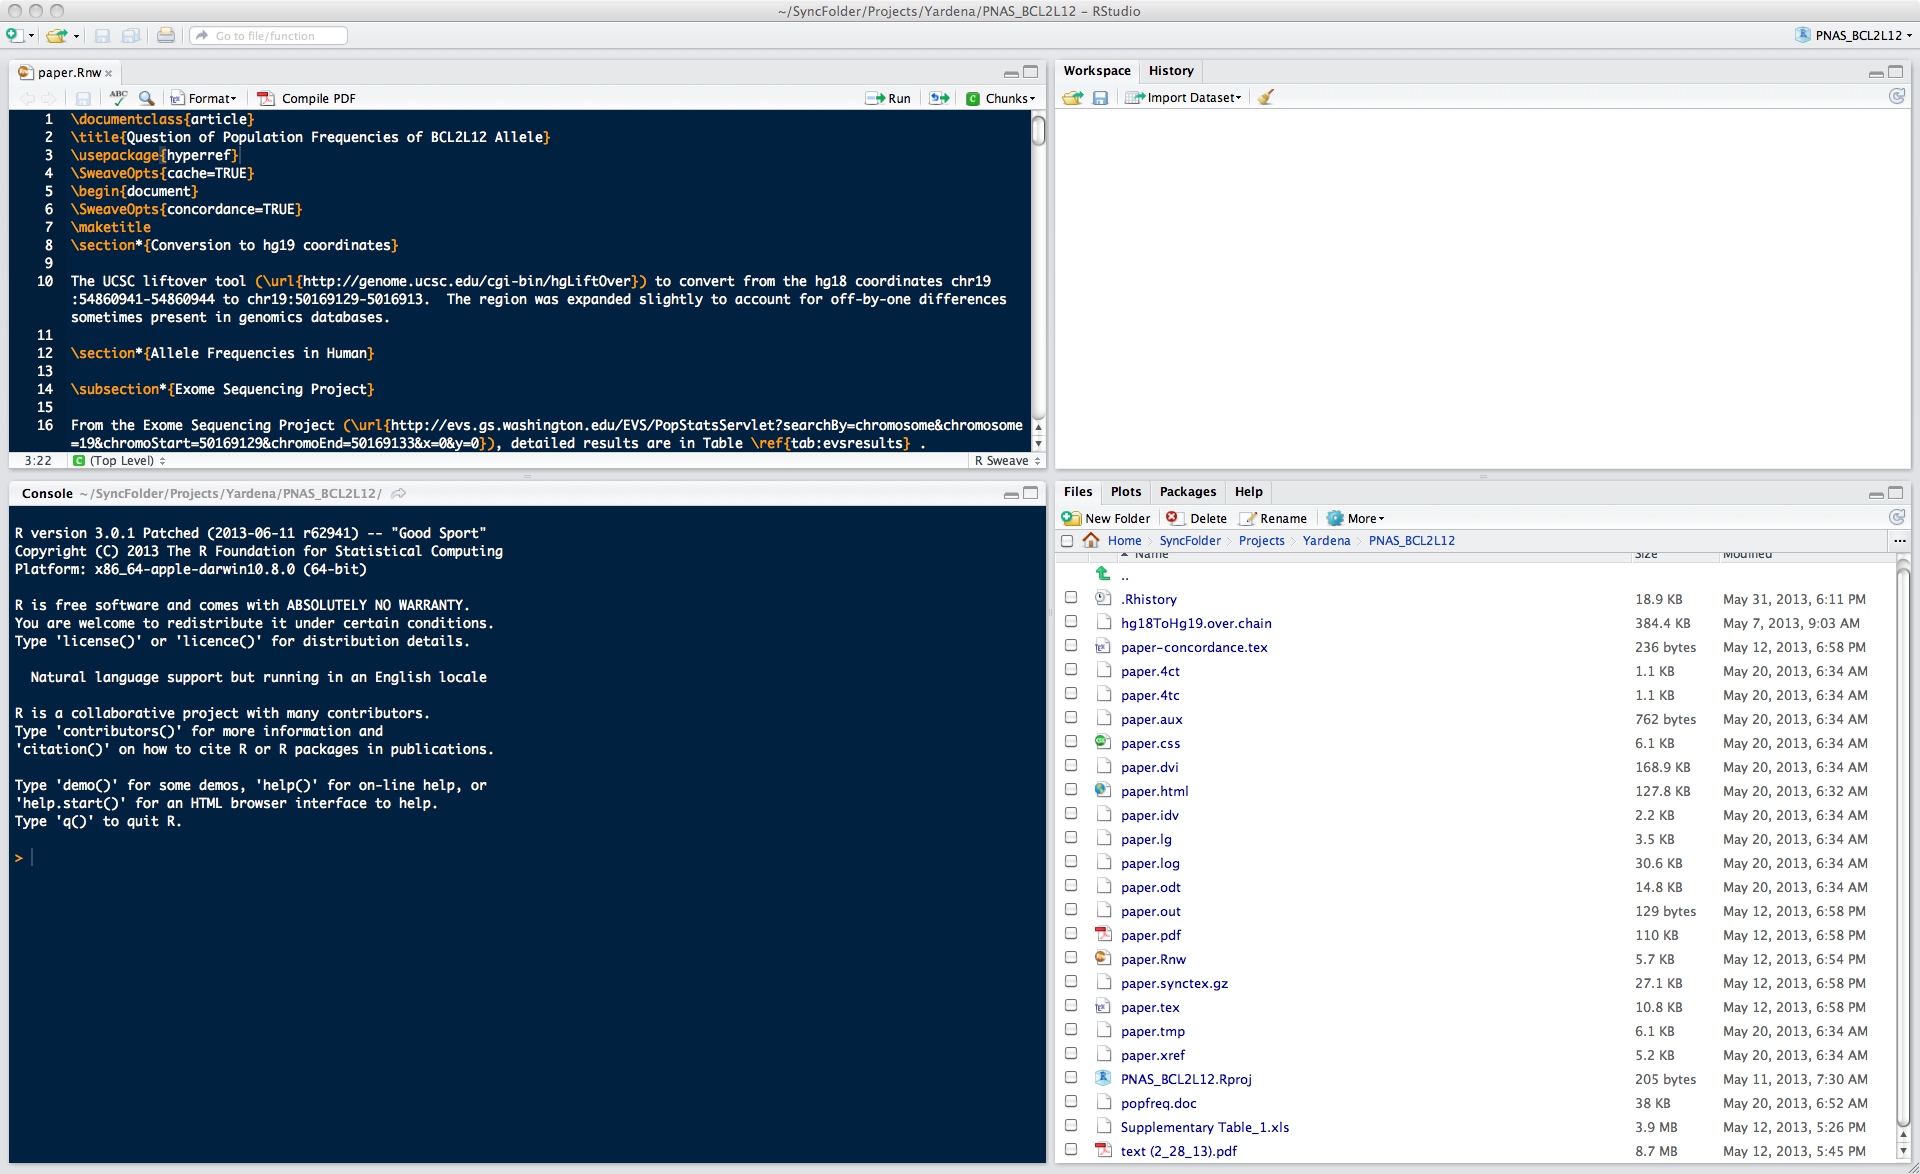
\includegraphics[width=26.67in]{images/RStudio} \caption{The Rstudio interface}\label{fig:rstudiointerface}
\end{figure}

\section{First steps}\label{first-steps}

\subsection{Interacting with R}\label{interacting-with-r}

The only meaningful way of interacting with R is by typing into the R
console. At the most basic level, anything that we type at the command
line will fall into one of two categories:

\begin{enumerate}
\def\labelenumi{\arabic{enumi}.}
\item
  Assignments

\begin{Shaded}
\begin{Highlighting}[]
\NormalTok{x =}\StringTok{ }\DecValTok{1}
\NormalTok{y <-}\StringTok{ }\DecValTok{2}
\end{Highlighting}
\end{Shaded}
\item
  Expressions

\begin{Shaded}
\begin{Highlighting}[]
\DecValTok{1} \OperatorTok{+}\StringTok{ }\NormalTok{pi }\OperatorTok{+}\StringTok{ }\KeywordTok{sin}\NormalTok{(}\DecValTok{42}\NormalTok{)}
\end{Highlighting}
\end{Shaded}

\begin{verbatim}
## [1] 3.225071
\end{verbatim}
\end{enumerate}

The assignment type is obvious because either the The ``\textless{}-''
or ``='' are used. Note that when we type expressions, R will return a
result. In this case, the result of R evaluating
\texttt{1\ +\ pi\ +\ sin(42)} is \texttt{3.2250711}.

The standard R prompt is a ``\textgreater{}'' sign. When present, R is
waiting for the next expression or assignment. If a line is not a
complete R command, R will continue the next line with a ``+''. For
example, typing the fillowing with a ``Return'' after the second ``+''
will result in R giving back a ``+'' on the next line, a prompt to keep
typing.

\begin{Shaded}
\begin{Highlighting}[]
\DecValTok{1} \OperatorTok{+}\StringTok{ }\NormalTok{pi }\OperatorTok{+}
\KeywordTok{sin}\NormalTok{(}\FloatTok{3.7}\NormalTok{)}
\end{Highlighting}
\end{Shaded}

\begin{verbatim}
## [1] 3.611757
\end{verbatim}

\subsection{Rules for Names in R}\label{rules-for-names-in-r}

R allows users to assign names to objects such as variables, functions,
and even dimensions of data. However, these names must follow a few
rules.

\begin{itemize}
\tightlist
\item
  Names may contain any combination of letters, numbers, underscore, and
  ``.''
\item
  Names may not start with numbers, underscore.
\item
  R names are case-sensitive.
\end{itemize}

Examples of valid R names include:

\begin{verbatim}
    pi
    x
    camelCaps
    my_stuff
    MY_Stuff
    this.is.the.name.of.the.man
    ABC123
    abc1234asdf
    .hi
\end{verbatim}

\subsection{Resources for Getting
Help}\label{resources-for-getting-help}

There is extensive built-in help and documentation within R.

If the name of the function or object on which help is sought is known,
the following approaches with the name of the function or object will be
helpful. For a concrete example, examine the help for the \texttt{print}
method.

\begin{Shaded}
\begin{Highlighting}[]
\KeywordTok{help}\NormalTok{(print)}
\KeywordTok{help}\NormalTok{(}\StringTok{'print'}\NormalTok{)}
\NormalTok{?print}
\end{Highlighting}
\end{Shaded}

If the name of the function or object on which help is sought is
\emph{not} known, the following from within R will be helpful.

\begin{Shaded}
\begin{Highlighting}[]
\KeywordTok{help.search}\NormalTok{(}\StringTok{'microarray'}\NormalTok{)}
\KeywordTok{RSiteSearch}\NormalTok{(}\StringTok{'microarray'}\NormalTok{)}
\end{Highlighting}
\end{Shaded}

There are also tons of online resources that Google will include in
searches if online searching feels more appropriate.

I strongly recommend using \texttt{help(newfunction)} for all functions
that are new or unfamiliar to you.

\section{Introduction to R data
structures}\label{introduction-to-r-data-structures}

As in many programming languages, understanding how data are stored and
manipulated is important to getting the most out of the experience. In
these next few sections, we will introduce some basic R data types and
structures as well as some general approaches for working with them.

\subsection{Vectors}\label{vectors}

In R, even a single value is a vector with length=1.

\begin{Shaded}
\begin{Highlighting}[]
\NormalTok{z =}\StringTok{ }\DecValTok{1}
\NormalTok{z}
\end{Highlighting}
\end{Shaded}

\begin{verbatim}
## [1] 1
\end{verbatim}

\begin{Shaded}
\begin{Highlighting}[]
\KeywordTok{length}\NormalTok{(z)}
\end{Highlighting}
\end{Shaded}

\begin{verbatim}
## [1] 1
\end{verbatim}

In the code above, we ``assigned'' the value 1 to the variable named
\texttt{z}. Typing \texttt{z} by itself is an ``expression'' that
returns a result which is, in this case, the value that we just
assigned. The \texttt{length} method takes an R object and returns the R
length. There are numerous ways of asking R about what an object
represents, and \texttt{length} is one of them.

Vectors can contain numbers, strings (character data), or logical values
(\texttt{TRUE} and \texttt{FALSE}) or other ``atomic'' data types (table
\ref{tab:simpletypes}). \emph{Vectors cannot contain a mix of types!} We
will introduce another data structure, the R \texttt{list} for
situations when we need to store a mix of base R data types.

\begin{longtable}[]{@{}ll@{}}
\caption{\label{tab:simpletypes} Atomic (simplest) data types in
R.}\tabularnewline
\toprule
Data type & Stores\tabularnewline
\midrule
\endfirsthead
\toprule
Data type & Stores\tabularnewline
\midrule
\endhead
numeric & floating point numbers\tabularnewline
integer & integers\tabularnewline
complex & complex numbers\tabularnewline
factor & categorical data\tabularnewline
character & strings\tabularnewline
logical & TRUE or FALSE\tabularnewline
NA & missing\tabularnewline
NULL & empty\tabularnewline
function & function type\tabularnewline
\bottomrule
\end{longtable}

\subsubsection{Creating vectors}\label{creating-vectors}

Character vectors (also sometimes called ``string'' vectors) are entered
with each value surrounded by single or double quotes; either is
acceptable, but they must match. They are always displayed by R with
double quotes. Here are some examples of creating vectors:

\begin{Shaded}
\begin{Highlighting}[]
\CommentTok{# examples of vectors}
\KeywordTok{c}\NormalTok{(}\StringTok{'hello'}\NormalTok{,}\StringTok{'world'}\NormalTok{)}
\end{Highlighting}
\end{Shaded}

\begin{verbatim}
## [1] "hello" "world"
\end{verbatim}

\begin{Shaded}
\begin{Highlighting}[]
\KeywordTok{c}\NormalTok{(}\DecValTok{1}\NormalTok{,}\DecValTok{3}\NormalTok{,}\DecValTok{4}\NormalTok{,}\DecValTok{5}\NormalTok{,}\DecValTok{1}\NormalTok{,}\DecValTok{2}\NormalTok{)}
\end{Highlighting}
\end{Shaded}

\begin{verbatim}
## [1] 1 3 4 5 1 2
\end{verbatim}

\begin{Shaded}
\begin{Highlighting}[]
\KeywordTok{c}\NormalTok{(}\FloatTok{1.12341e7}\NormalTok{,}\FloatTok{78234.126}\NormalTok{)}
\end{Highlighting}
\end{Shaded}

\begin{verbatim}
## [1] 11234100.00    78234.13
\end{verbatim}

\begin{Shaded}
\begin{Highlighting}[]
\KeywordTok{c}\NormalTok{(}\OtherTok{TRUE}\NormalTok{,}\OtherTok{FALSE}\NormalTok{,}\OtherTok{TRUE}\NormalTok{,}\OtherTok{TRUE}\NormalTok{)}
\end{Highlighting}
\end{Shaded}

\begin{verbatim}
## [1]  TRUE FALSE  TRUE  TRUE
\end{verbatim}

\begin{Shaded}
\begin{Highlighting}[]
\CommentTok{# note how in the next case the TRUE is converted to "TRUE"}
\CommentTok{# with quotes around it.}
\KeywordTok{c}\NormalTok{(}\OtherTok{TRUE}\NormalTok{,}\StringTok{'hello'}\NormalTok{)}
\end{Highlighting}
\end{Shaded}

\begin{verbatim}
## [1] "TRUE"  "hello"
\end{verbatim}

We can also create vectors as ``regular sequences'' of numbers. For
example:

\begin{Shaded}
\begin{Highlighting}[]
\CommentTok{# create a vector of integers from 1 to 10}
\NormalTok{x =}\StringTok{ }\DecValTok{1}\OperatorTok{:}\DecValTok{10}
\CommentTok{# and backwards}
\NormalTok{x =}\StringTok{ }\DecValTok{10}\OperatorTok{:}\DecValTok{1}
\end{Highlighting}
\end{Shaded}

The \texttt{seq} function can create more flexible regular sequences.
You \emph{did} read the help for \texttt{seq}, right?

\begin{Shaded}
\begin{Highlighting}[]
\CommentTok{# create a vector of numbers from 1 to 4 skipping by 0.3}
\NormalTok{y =}\StringTok{ }\KeywordTok{seq}\NormalTok{(}\DecValTok{1}\NormalTok{,}\DecValTok{4}\NormalTok{,}\FloatTok{0.3}\NormalTok{)}
\end{Highlighting}
\end{Shaded}

And creating a new vector by concatenating existing vectors is possible,
as well.

\begin{Shaded}
\begin{Highlighting}[]
\CommentTok{# create a sequence by concatenating two other sequences}
\NormalTok{z =}\StringTok{ }\KeywordTok{c}\NormalTok{(y,x)}
\NormalTok{z}
\end{Highlighting}
\end{Shaded}

\begin{verbatim}
##  [1]  1.0  1.3  1.6  1.9  2.2  2.5  2.8  3.1  3.4  3.7  4.0 10.0  9.0  8.0
## [15]  7.0  6.0  5.0  4.0  3.0  2.0  1.0
\end{verbatim}

\subsubsection{Vector Operations}\label{vector-operations}

Operations on a single vector are typically done element-by-element. For
example, we can add \texttt{2} to a vector, \texttt{2} is added to each
element of the vector and a new vector of the same length is returned.

\begin{Shaded}
\begin{Highlighting}[]
\NormalTok{x =}\StringTok{ }\DecValTok{1}\OperatorTok{:}\DecValTok{10}
\NormalTok{x }\OperatorTok{+}\StringTok{ }\DecValTok{2}
\end{Highlighting}
\end{Shaded}

\begin{verbatim}
##  [1]  3  4  5  6  7  8  9 10 11 12
\end{verbatim}

If the operation involves two vectors, the following rules apply. If the
vectors are the same length: R simply applies the operation to each pair
of elements.

\begin{Shaded}
\begin{Highlighting}[]
\NormalTok{x }\OperatorTok{+}\StringTok{ }\NormalTok{x}
\end{Highlighting}
\end{Shaded}

\begin{verbatim}
##  [1]  2  4  6  8 10 12 14 16 18 20
\end{verbatim}

If the vectors are different lengths, but one length a multiple of the
other, R reuses the shorter vector as needed.

\begin{Shaded}
\begin{Highlighting}[]
\NormalTok{x =}\StringTok{ }\DecValTok{1}\OperatorTok{:}\DecValTok{10}
\NormalTok{y =}\StringTok{ }\KeywordTok{c}\NormalTok{(}\DecValTok{1}\NormalTok{,}\DecValTok{2}\NormalTok{)}
\NormalTok{x }\OperatorTok{*}\StringTok{ }\NormalTok{y}
\end{Highlighting}
\end{Shaded}

\begin{verbatim}
##  [1]  1  4  3  8  5 12  7 16  9 20
\end{verbatim}

If the vectors are different lengths, but one length \emph{not} a
multiple of the other, R reuses the shorter vector as needed \emph{and}
delivers a warning.

\begin{Shaded}
\begin{Highlighting}[]
\NormalTok{x =}\StringTok{ }\DecValTok{1}\OperatorTok{:}\DecValTok{10}
\NormalTok{y =}\StringTok{ }\KeywordTok{c}\NormalTok{(}\DecValTok{2}\NormalTok{,}\DecValTok{3}\NormalTok{,}\DecValTok{4}\NormalTok{)}
\NormalTok{x }\OperatorTok{*}\StringTok{ }\NormalTok{y}
\end{Highlighting}
\end{Shaded}

\begin{verbatim}
## Warning in x * y: longer object length is not a multiple of shorter object
## length
\end{verbatim}

\begin{verbatim}
##  [1]  2  6 12  8 15 24 14 24 36 20
\end{verbatim}

\begin{itemize}
\tightlist
\item
  {Typical operations include multiplication (``*''), addition,
  subtraction, division, exponentiation (`` \^{}''), but many operations
  in R operate on vectors and are then called ``vectorized''.}
\end{itemize}

\subsection{Summary of Simple Data
Types}\label{summary-of-simple-data-types}

\begin{longtable}[]{@{}cc@{}}
\toprule
Data type & Stores\tabularnewline
\midrule
\endhead
real & floating point numbers\tabularnewline
integer & integers\tabularnewline
complex & complex numbers\tabularnewline
factor & categorical data\tabularnewline
character & strings\tabularnewline
logical & TRUE or FALSE\tabularnewline
NA & missing\tabularnewline
NULL & empty\tabularnewline
function & function type\tabularnewline
\bottomrule
\end{longtable}

\subsubsection{Logical Vectors}\label{logical-vectors}

Logical vectors are vectors composed on only the values \texttt{TRUE}
and \texttt{FALSE}. Note the all-upper-case and no quotation marks.

\begin{verbatim}
a = c(TRUE,FALSE,TRUE)
# we can also create a logical vector from a numeric vector
# 0 = false, everything else is 1
b = c(1,0,217)
d = as.logical(b)
d
## [1]  TRUE FALSE  TRUE
# test if a and d are the same at every element
all.equal(a,d)
## [1] TRUE
# We can also convert from logical to numeric
as.numeric(a)
## [1] 1 0 1
\end{verbatim}

\subsubsection{Logical Operators}\label{logical-operators}

Some operators like
\texttt{\textless{},\ \textgreater{},\ ==,\ \textgreater{}=,\ \textless{}=,\ !=}
can be used to create logical vectors.

\begin{verbatim}
# create a numeric vector
x = 1:10
# testing whether x > 5 creates a logical vector
x > 5
##  [1] FALSE FALSE FALSE FALSE FALSE  TRUE  TRUE  TRUE  TRUE  TRUE
x <= 5
##  [1]  TRUE  TRUE  TRUE  TRUE  TRUE FALSE FALSE FALSE FALSE FALSE
x != 5
##  [1]  TRUE  TRUE  TRUE  TRUE FALSE  TRUE  TRUE  TRUE  TRUE  TRUE
x == 5
##  [1] FALSE FALSE FALSE FALSE  TRUE FALSE FALSE FALSE FALSE FALSE
# we can also assign the results to a variable
y = (x == 5)
y
##  [1] FALSE FALSE FALSE FALSE  TRUE FALSE FALSE FALSE FALSE FALSE
\end{verbatim}

\subsection{Indexing Vectors}\label{indexing-vectors}

\subsubsection{Indexing Vectors}\label{indexing-vectors-1}

\begin{itemize}
\item
  {In programming, an index is used to refer to a specific element or
  set of elements in an vector (or other data structure).}
\item
  {R uses \texttt{{[}} and \texttt{{]}} to perform indexing.}

\begin{verbatim}
x = seq(0,1,0.1)
# create a new vector from the 4th element of x
x[4]
## [1] 0.3
\end{verbatim}
\item
  {Indexing can use other vectors for the indexing}

\begin{verbatim}
x[c(3,5,6)]
## [1] 0.2 0.4 0.5
y = 3:6
x[y]
## [1] 0.2 0.3 0.4 0.5
\end{verbatim}
\end{itemize}

\subsubsection{Indexing Vectors and Logical
Vectors}\label{indexing-vectors-and-logical-vectors}

Combining the concept of indexing with the concept of logical vectors
results in a very power combination.

\begin{verbatim}
# use help('rnorm') to figure out what is happening next
myvec = rnorm(10)
# create logical vector that is TRUE where myvec is >0.25
gt1 = (myvec > 0.25)
sum(gt1)
## [1] 2
# and use our logical vector to create a vector of myvec values that are >0.25
myvec[gt1]
## [1] 0.8500783 1.2182233
# or <=0.25 using the logical "not" operator, "!"
myvec[!gt1]
## [1] -0.52361528 -1.96734990  0.09722437 -0.09474050 -0.92634247  0.10862202
## [7] -0.01423129 -1.10639317
# shorter, one line approach
myvec[myvec > 0.25]
## [1] 0.8500783 1.2182233
\end{verbatim}

\subsection{String Handling in R}\label{string-handling-in-r}

\subsubsection{Concatenating Strings}\label{concatenating-strings}

R uses the \texttt{paste} function to concatenate strings.

\begin{verbatim}
paste("abc","def")
## [1] "abc def"
paste("abc","def",sep="THISSEP")
## [1] "abcTHISSEPdef"
paste0("abc","def")
## [1] "abcdef"
paste(c("X","Y"),1:10)
##  [1] "X 1"  "Y 2"  "X 3"  "Y 4"  "X 5"  "Y 6"  "X 7"  "Y 8"  "X 9"  "Y 10"
paste(c("X","Y"),1:10,sep="_")
##  [1] "X_1"  "Y_2"  "X_3"  "Y_4"  "X_5"  "Y_6"  "X_7"  "Y_8"  "X_9"  "Y_10"
\end{verbatim}

\subsubsection{More String Functions}\label{more-string-functions}

\begin{itemize}
\item
  {Number of characters in a string}

\begin{verbatim}
nchar('abc')
## [1] 3
nchar(c('abc','d',123456))
## [1] 3 1 6
\end{verbatim}
\item
  {Extract substrings}

\begin{verbatim}
substr('This is a good sentence.',start=10,stop=15)
## [1] " good "
\end{verbatim}
\item
  {String replacement}

\begin{verbatim}
sub('This','That','This is a good sentence.')
## [1] "That is a good sentence."
\end{verbatim}
\item
  {Finding matching strings}

\begin{verbatim}
grep('bcd',c('abcdef','abcd','bcde','cdef','defg'))
## [1] 1 2 3
grep('bcd',c('abcdef','abcd','bcde','cdef','defg'),value=TRUE)
## [1] "abcdef" "abcd"   "bcde"
\end{verbatim}
\end{itemize}

\subsection{Special Data Types}\label{special-data-types}

\subsubsection{\texorpdfstring{Missing Values, AKA
``NA''}{Missing Values, AKA NA}}\label{missing-values-aka-na}

R has a special value, ``NA'', that represents a ``missing'' value in a
vector or other data structure.

\begin{verbatim}
x = 1:5
x
## [1] 1 2 3 4 5
length(x)
## [1] 5
is.na(x)
## [1] FALSE FALSE FALSE FALSE FALSE
x[2] = NA
x
## [1]  1 NA  3  4  5
length(x)
## [1] 5
is.na(x)
## [1] FALSE  TRUE FALSE FALSE FALSE
x[!is.na(x)]
## [1] 1 3 4 5
\end{verbatim}

\subsubsection{Factors}\label{factors}

\begin{itemize}
\item
  {A factor is a special type of vector, normally used to hold a
  categorical variable in many statistical functions.}
\item
  {Such vectors have class ``factor''.}
\item
  {Factors are primarily used in Analysis of Variance (ANOVA). When a
  factor is used as a predictor variable, the corresponding indicator
  variables are created.}
\end{itemize}

{Note of caution} Factors in R often \emph{appear} to be character
vectors when printed, but you will notice that they do not have double
quotes around them. They are stored in R as numbers with a key name, so
sometimes you will note that the factor \emph{behaves} like a numeric
vector.

\subsubsection{Factors in Practice}\label{factors-in-practice}

\begin{verbatim}
# create the character vector
citizen<-c("uk","us","no","au","uk","us","us","no","au") 
# convert to factor
citizenf<-factor(citizen)                                
citizen             
## [1] "uk" "us" "no" "au" "uk" "us" "us" "no" "au"
citizenf
## [1] uk us no au uk us us no au
## Levels: au no uk us
# convert factor back to character vector
as.character(citizenf)
## [1] "uk" "us" "no" "au" "uk" "us" "us" "no" "au"
# convert to numeric vector
as.numeric(citizenf)
## [1] 3 4 2 1 3 4 4 2 1
\end{verbatim}

\subsubsection{Factors in Practice}\label{factors-in-practice-1}

\begin{verbatim}
# R stores many data structures as vectors with "attributes" and "class"
attributes(citizenf)
## \$levels
## [1] "au" "no" "uk" "us"
## 
## \$class
## [1] "factor"
class(citizenf)
## [1] "factor"
# note that after unclassing, we can see the 
# underlying numeric structure again
unclass(citizenf)
## [1] 3 4 2 1 3 4 4 2 1
## attr(,"levels")
## [1] "au" "no" "uk" "us"
table(citizenf)
## citizenf
## au no uk us 
##  2  2  2  3
\end{verbatim}

\section{Rectangular Data}\label{rectangular-data}

\subsubsection{Matrices and Data Frames}\label{matrices-and-data-frames}

\begin{itemize}
\item
  {A matrix is a rectangular array. It can be viewed as a collection of
  column vectors all of the same length and the same type (i.e.~numeric,
  character or logical).}
\item
  {A data frame is \emph{also} a rectangular array. All of the columns
  must be the same length, but they may be of \emph{different} types.}
\item
  {The rows and columns of a matrix or data frame can be given names.}
\item
  {However these are implemented differently in R; many operations will
  work for one but not both.}
\end{itemize}

\subsection{Matrix Operations}\label{matrix-operations}

\subsubsection{Matrix Operations}\label{matrix-operations-1}

\begin{verbatim}
x<-1:10 
y<-rnorm(10)
# make a matrix by column binding two numeric vectors
mat<-cbind(x,y)
mat
##        x          y
##  [1,]  1  0.3842634
##  [2,]  2 -1.2536470
##  [3,]  3 -1.4098608
##  [4,]  4  1.7139083
##  [5,]  5 -0.1876347
##  [6,]  6 -0.3343492
##  [7,]  7  1.6553040
##  [8,]  8  0.5974976
##  [9,]  9 -1.8443792
## [10,] 10  1.4203497
# And the names of the rows and columns
rownames(mat)
## NULL
colnames(mat)
## [1] "x" "y"
\end{verbatim}

\subsubsection{Matrix Operations}\label{matrix-operations-2}

Indexing for matrices works as for vectors except that we now need to
include both the row and column (in that order).

\begin{verbatim}
# The 2nd element of the 1st row of mat
mat[1,2]
##         y 
## 0.3842634
# The first ROW of mat
mat[1,]
##         x         y 
## 1.0000000 0.3842634
# The first COLUMN of mat
mat[,1]
##  [1]  1  2  3  4  5  6  7  8  9 10
# and all elements of mat that are > 4; note no comma
mat[mat>4]
## [1]  5  6  7  8  9 10
\end{verbatim}

\subsubsection{Matrix Operations}\label{matrix-operations-3}

\begin{verbatim}
# create a matrix with 2 columns and 10 rows
# filled with random normal deviates
m = matrix(rnorm(20),nrow=10)
# multiply all values in the matrix by 20
m = m*20
# and add 100 to the first column of m
m[,1] = m[,1] + 100
# summarize m
summary(m)
##        V1               V2          
##  Min.   : 44.58   Min.   :-42.4628  
##  1st Qu.: 93.26   1st Qu.:-19.8712  
##  Median :100.72   Median :  3.6691  
##  Mean   : 95.27   Mean   : -0.4271  
##  3rd Qu.:106.33   3rd Qu.: 17.3559  
##  Max.   :111.29   Max.   : 31.2418
\end{verbatim}

\subsection{Data Frames}\label{data-frames}

\subsubsection{Matrices Versus Data
Frames}\label{matrices-versus-data-frames}

\begin{verbatim}
mat<-cbind(x,y)
class(mat[,1])          
## [1] "numeric"
z = paste0('a',1:10)
tab<-cbind(x,y,z)
class(tab)
## [1] "matrix"
mode(tab[,1])
## [1] "character"
head(tab,4)
##      x   y                   z   
## [1,] "1" "0.384263423333191" "a1"
## [2,] "2" "-1.25364703104426" "a2"
## [3,] "3" "-1.40986082624299" "a3"
## [4,] "4" "1.7139082579506"   "a4"
\end{verbatim}

\subsubsection{Matrices Versus Data
Frames}\label{matrices-versus-data-frames-1}

\begin{verbatim}
tab<-data.frame(x,y,z)
class(tab)
## [1] "data.frame"
head(tab)
##   x          y  z
## 1 1  0.3842634 a1
## 2 2 -1.2536470 a2
## 3 3 -1.4098608 a3
## 4 4  1.7139083 a4
## 5 5 -0.1876347 a5
## 6 6 -0.3343492 a6
mode(tab[,1])
## [1] "numeric"
class(tab[,3])
## [1] "factor"
rownames(tab)           
##  [1] "1"  "2"  "3"  "4"  "5"  "6"  "7"  "8"  "9"  "10"
rownames(tab)<-paste0("row",1:10)
rownames(tab)
##  [1] "row1"  "row2"  "row3"  "row4"  "row5"  "row6"  "row7"  "row8" 
##  [9] "row9"  "row10"
\end{verbatim}

\subsubsection{Data Frames, Continued}\label{data-frames-continued}

\begin{itemize}
\item
  {Data frame columns can be refered to by name using the ``dollar
  sign'' operator}

\begin{verbatim}
tab\$x
##  [1]  1  2  3  4  5  6  7  8  9 10
tab\$y
##  [1]  0.3842634 -1.2536470 -1.4098608  1.7139083 -0.1876347 -0.3343492
##  [7]  1.6553040  0.5974976 -1.8443792  1.4203497
\end{verbatim}
\item
  {Column names can be set, which can be useful for referring to data
  later}

\begin{verbatim}
colnames(tab)
## [1] "x" "y" "z"
colnames(tab) = paste0('col',1:3)
\end{verbatim}
\end{itemize}

\subsubsection{Exercise: Subsetting Data
Frames}\label{exercise-subsetting-data-frames}

Try these

\begin{verbatim}
ncol(tab)
nrow(tab)
dim(tab)
summary(tab)
tab[1:3,]
tab[,2:3]
tab[,1]>7
tab[tab[,1]>7,]
tab[tab[,1]>7,3]
tab[tab[,1]>7,2:3]
tab[tab\$x>7,3]
tab\$z[tab\$x>3]
\end{verbatim}

\subsection{Basic Textual Input and
Output}\label{basic-textual-input-and-output}

\subsubsection{Reading and Writing Data Frames to
Disk}\label{reading-and-writing-data-frames-to-disk}

\begin{itemize}
\item
  {The \texttt{write.table} function and friends write a data.frame or
  matrix to disk as a text file.}

\begin{verbatim}
write.table(tab,file='tab.txt',sep="\t",col.names=TRUE)
# remove tab from the workspace
rm(tab)
# make sure it is gone
ls(pattern="tab")
## character(0)
\end{verbatim}
\item
  {The \texttt{read.table} function and friends read a data.frame or
  matrix from a text file.}

\begin{verbatim}
tab = read.table('tab.txt',sep="\t",header=TRUE)
head(tab,3)
##      col1       col2 col3
## row1    1  0.3842634   a1
## row2    2 -1.2536470   a2
## row3    3 -1.4098608   a3
\end{verbatim}
\end{itemize}

\subsection{Lists and Objects}\label{lists-and-objects}

\subsubsection{Lists}\label{lists}

\begin{itemize}
\item
  {A list is a collection of objects that may be the same or different
  types.}
\item
  {[}The objects generally have names, and may be indexed either by name
  (e.g.~my.list\$name3) or component number (e.g.~my.list{[}{[}3{]}{]})
\item
  {A data frame is a list of matched column vectors.}
\end{itemize}

\subsubsection{Lists in Practice}\label{lists-in-practice}

\begin{itemize}
\item
  {Create a list, noting the different data types involved.}

\begin{verbatim}
a = list(1,"b",c(1,2,3))
a
## [[1]]
## [1] 1
## 
## [[2]]
## [1] "b"
## 
## [[3]]
## [1] 1 2 3
length(a)
## [1] 3
class(a)
## [1] "list"
a[[3]]
## [1] 1 2 3
\end{verbatim}
\end{itemize}

\subsubsection{Lists in Practice}\label{lists-in-practice-1}

\begin{itemize}
\item
  {A data frame \emph{is} a list.}

\begin{verbatim}
# test if our friend "tab" is a list
is.list(tab)
## [1] TRUE
tab[[2]]
##  [1]  0.3842634 -1.2536470 -1.4098608  1.7139083 -0.1876347 -0.3343492
##  [7]  1.6553040  0.5974976 -1.8443792  1.4203497
names(tab)
## [1] "col1" "col2" "col3"
\end{verbatim}
\end{itemize}

\subsubsection{Summary of Simple Data
Types}\label{summary-of-simple-data-types-1}

\begin{longtable}[]{@{}cc@{}}
\toprule
Data type & Stores\tabularnewline
\midrule
\endhead
real & floating point numbers\tabularnewline
integer & integers\tabularnewline
complex & complex numbers\tabularnewline
factor & categorical data\tabularnewline
character & strings\tabularnewline
logical & TRUE or FALSE\tabularnewline
NA & missing\tabularnewline
NULL & empty\tabularnewline
function & function type\tabularnewline
\bottomrule
\end{longtable}

\subsubsection{Summary of Aggregate Data
Types}\label{summary-of-aggregate-data-types}

\begin{longtable}[]{@{}cc@{}}
\toprule
Data type & Stores\tabularnewline
\midrule
\endhead
vector & one-dimensional data, single data type\tabularnewline
matrix & two-dimensional data, single data type\tabularnewline
data frame & two-dimensional data, multiple data types\tabularnewline
list & list of data types, not all need to be the same
type\tabularnewline
object & a list with attributes and potentially slots and
methods\tabularnewline
\bottomrule
\end{longtable}

\section{Plotting and Graphics}\label{plotting-and-graphics}

\subsection{Basics of Plotting}\label{basics-of-plotting}

\subsubsection{Basic Plot Functions}\label{basic-plot-functions}

\begin{itemize}
\item
  {The command \texttt{plot(x,y)} will plot vector x as the independent
  variable and vector y as the dependent variable.}
\item
  {Within the command line, you can specify the title of the graph, the
  name of the x-axis, and the name of the y-axis.}

  \begin{itemize}
  \item
    {main='title'}
  \item
    {xlab='name of x axis'}
  \item
    {ylab='name of y axis'}
  \end{itemize}
\item
  {The command \texttt{lines(x,y)} adds a line segment to the plot.}
\item
  {The command \texttt{points(x,y)} adds points to the plot.}
\item
  {A legend can be created using \texttt{legend}.}
\end{itemize}

{demo}

\begin{verbatim}
demo(graphics)
\end{verbatim}

\subsubsection{Simple Plotting Example}\label{simple-plotting-example}

Try this yourself:

\begin{Shaded}
\begin{Highlighting}[]
\NormalTok{    x =}\StringTok{ }\DecValTok{1}\OperatorTok{:}\DecValTok{100}
\NormalTok{    y =}\StringTok{ }\KeywordTok{rnorm}\NormalTok{(}\DecValTok{100}\NormalTok{,}\DecValTok{3}\NormalTok{,}\DecValTok{1}\NormalTok{) }\CommentTok{# 100 random normal deviates with mean=3, sd=1}
    \KeywordTok{plot}\NormalTok{(x,y)}
\end{Highlighting}
\end{Shaded}

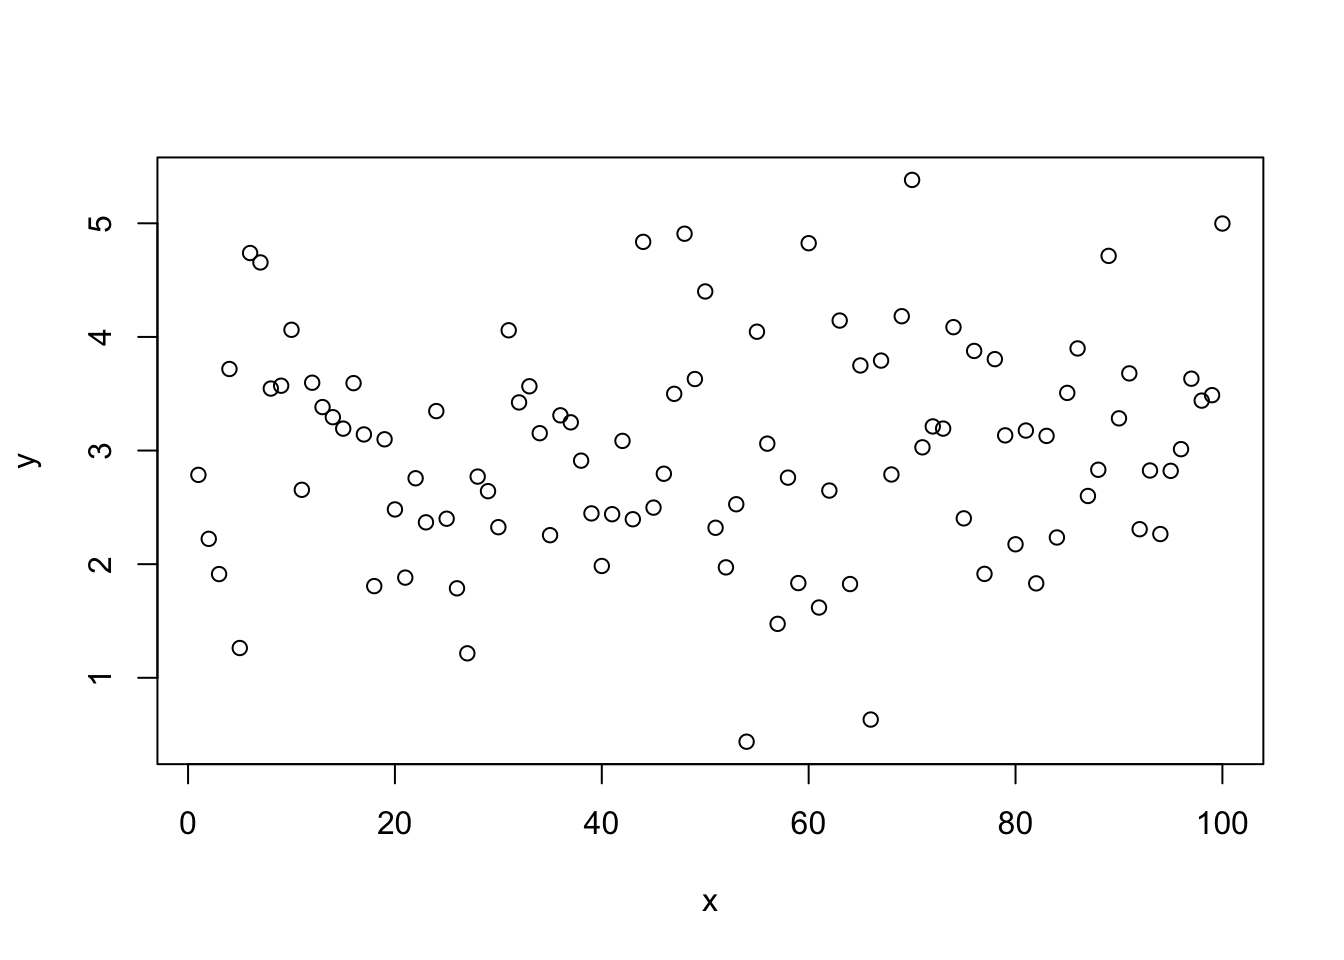
\includegraphics{_main_files/figure-latex/unnamed-chunk-15-1.pdf}

\begin{Shaded}
\begin{Highlighting}[]
    \KeywordTok{plot}\NormalTok{(x,y,}\DataTypeTok{main=}\StringTok{'My First Plot'}\NormalTok{)}
\end{Highlighting}
\end{Shaded}

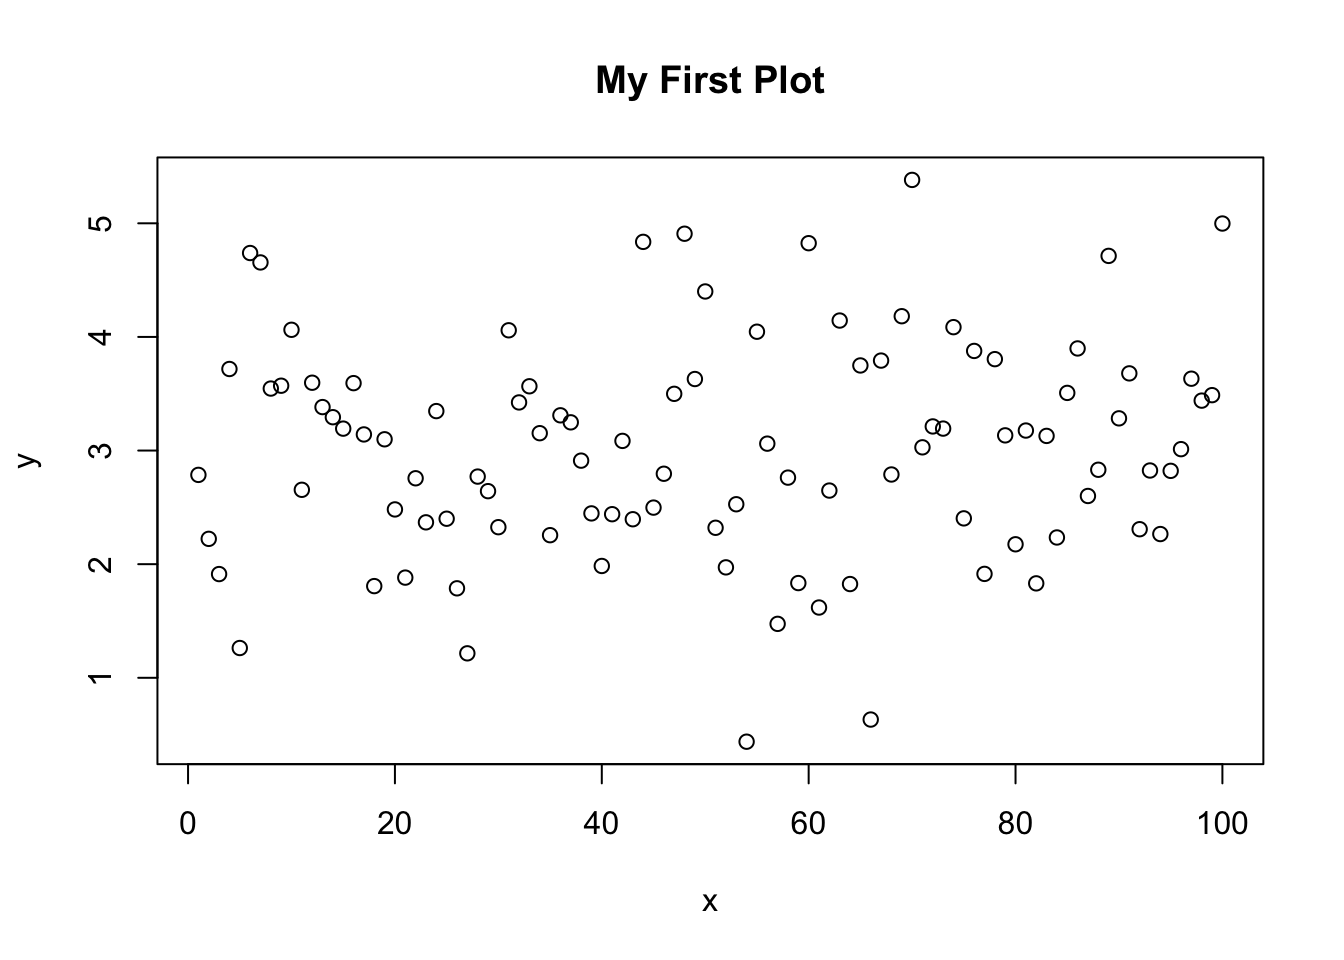
\includegraphics{_main_files/figure-latex/unnamed-chunk-16-1.pdf}

\begin{Shaded}
\begin{Highlighting}[]
    \CommentTok{# change point type}
    \KeywordTok{plot}\NormalTok{(x,y,}\DataTypeTok{pch=}\DecValTok{3}\NormalTok{)}
\end{Highlighting}
\end{Shaded}

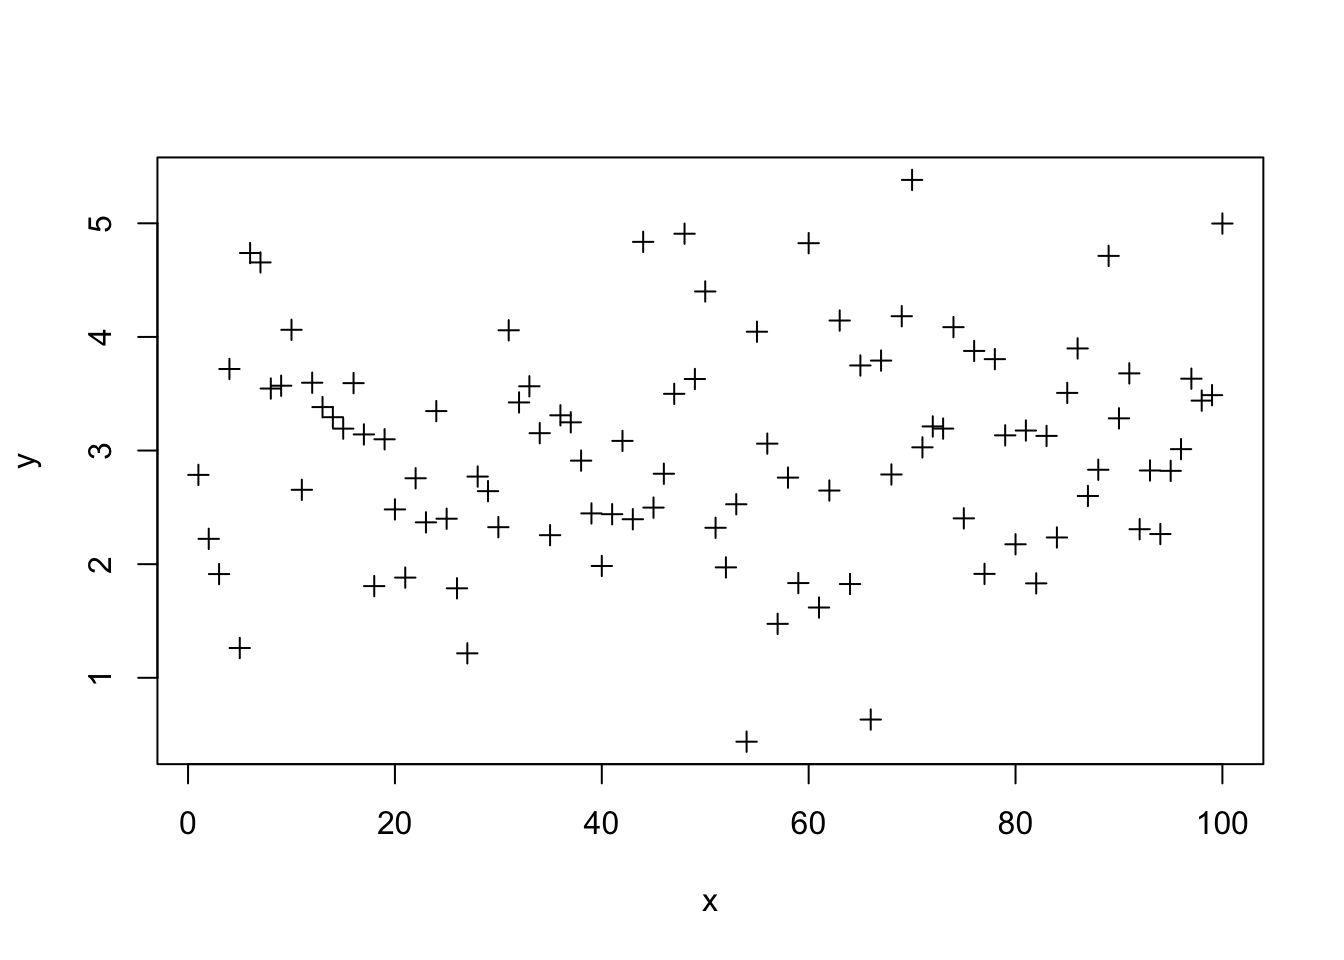
\includegraphics{_main_files/figure-latex/unnamed-chunk-17-1.pdf}

\begin{Shaded}
\begin{Highlighting}[]
    \CommentTok{# change color}
    \KeywordTok{plot}\NormalTok{(x,y,}\DataTypeTok{pch=}\DecValTok{4}\NormalTok{,}\DataTypeTok{col=}\DecValTok{2}\NormalTok{)}
    \CommentTok{# draw lines between points}
    \KeywordTok{lines}\NormalTok{(x,y,}\DataTypeTok{col=}\DecValTok{3}\NormalTok{)}
\end{Highlighting}
\end{Shaded}

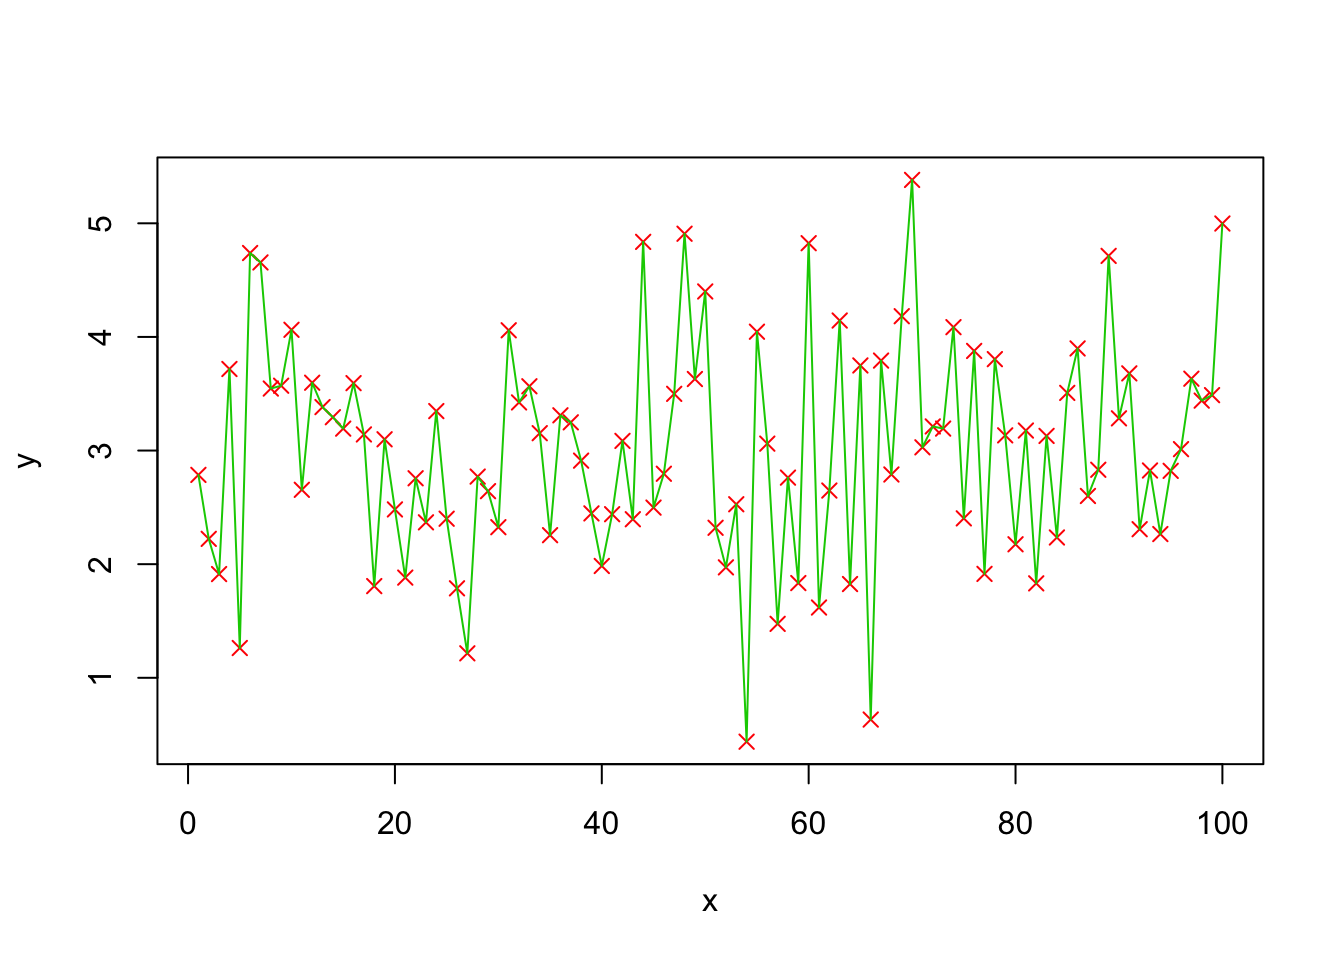
\includegraphics{_main_files/figure-latex/unnamed-chunk-18-1.pdf}

\subsubsection{More Plotting}\label{more-plotting}

\begin{verbatim}
z=sort(y)
# plot a sorted variable vs x
plot(x,z,main='Random Normal Numbers',
xlab='Index',ylab='Random Number')


# another example
plot(-4:4,-4:4) 
# and add a point at (0,2) to the plot
points(0,2,pch=6,col=12)
\end{verbatim}

\subsubsection{More Plotting}\label{more-plotting-1}

\begin{verbatim}
# check margin and outer margin settings
par(c("mar", "oma")) 
plot(x,y)
par(oma=c(1,1,1,1))  # set outer margin
plot(x,y)
par(mar=c(2.5,2.1,2.1,1)) # set margin
plot(x,y)


# A basic histogram
hist(z, main="Histogram",
    sub="Random normal")


# A "density" plot
plot(density(z), main="Density plot",
    sub="Random normal")


# A smaller "bandwidth" to capture more detail
plot(density(z, adjust=0.5),
  sub="smaller bandwidth")
\end{verbatim}

\subsubsection{Graphics Devices and Saving
Plots}\label{graphics-devices-and-saving-plots}

\begin{itemize}
\item
  {to make a plot directly to a file use: \texttt{png()},
  \texttt{postscript()}, etc.}
\item
  {R can have multiple graphics ``devices'' open.}

  \begin{itemize}
  \item
    {To see a list of active devices: \texttt{dev.list()}}
  \item
    {To close the most recent device: \texttt{dev.off()}}
  \item
    {To close device 5: \texttt{dev.off(5)}}
  \item
    {To use device 5: \texttt{dev.set(5)}}
  \end{itemize}
\end{itemize}

\subsubsection{More Plotting}\label{more-plotting-2}

\begin{itemize}
\item
  {Save a png image to a file}

\begin{verbatim}
png(file="myplot.png",width=480,height=480)
plot(density(z,adjust=2.0),sub="larger bandwidth")
dev.off()
\end{verbatim}
\item
  {On your own, save a pdf to a file. NOTE: The dimensions in
  \texttt{pdf()} are in \emph{inches}}
\item
  {Multiple plots on the same page:}

\begin{verbatim}
par(mfrow=c(2,1))
plot(density(z,adjust=2.0),sub="larger bandwidth")
hist(z)


# use dev.off() to turn off the two-row plotting
\end{verbatim}
\end{itemize}

\subsubsection{R Graphics Galleries and
Resources}\label{r-graphics-galleries-and-resources}

Visit these sites for some ideas.

\begin{itemize}
\item
  {\url{http://www.sr.bham.ac.uk/~ajrs/R/r-gallery.html}}
\item
  {\url{http://gallery.r-enthusiasts.com/}}
\item
  {\url{http://cran.r-project.org/web/views/Graphics.html}}
\end{itemize}

\section{Control Structures, Looping, and
Applying}\label{control-structures-looping-and-applying}

\subsection{Control Structures and
Looping}\label{control-structures-and-looping}

\subsubsection{Control Structures in R}\label{control-structures-in-r}

\begin{itemize}
\item
  {R has multiple types of control structures that allows for sequential
  evaluation of statements.}
\item
  {For loops}

\begin{verbatim}
for (x in set) {operations}
\end{verbatim}
\item
  {while loops}

\begin{verbatim}
while (x in condition){operations}
\end{verbatim}
\item
  {If statements (conditional)}

\begin{verbatim}
if (condition) {
some operations 
 } else { other operations }
\end{verbatim}
\end{itemize}

\subsubsection{Control Structure and Looping
Examples}\label{control-structure-and-looping-examples}

\begin{verbatim}
x<-1:9
length(x)
# a simple conditional then two expressions
if (length(x)<=10) {
   x<-c(x,10:20);print(x)}
# more complex 
if (length(x)<5) {
    print(x)
} else {
    print(x[5:20])
}           
# print the values of x, one at a time
for (i in x) print(i) 
for(i in x) i   # note R will not echo in a loop
\end{verbatim}

\subsubsection{Control Structure and Looping
Examples}\label{control-structure-and-looping-examples-1}

\begin{verbatim}
# loop over a character vector
y<-c('a','b','hi there')            
for (i in y) print(i)

# and a while loop
j<-1                
while(j<10) { # do this while j<10      
  print(j)
  j<-j+2} # at each iteration, increase j by 2
\end{verbatim}

\subsection{Applying}\label{applying}

\subsubsection{Why Does R Have Apply
Functions}\label{why-does-r-have-apply-functions}

\begin{itemize}
\item
  {Often we want to apply the same function to all the rows or columns
  of a matrix, or all the elements of a list.}
\item
  {We could do this in a loop, but loops take a lot of time in an
  interpreted language like R.}
\item
  {R has more efficient built-in operators, the apply functions.}
\end{itemize}

{example} If mat is a matrix and fun is a function (such as mean, var,
lm \ldots{}) that takes a vector as its argument, then you can:

\begin{verbatim}
apply(mat,1,fun) # over rows--second argument is 1      
apply(mat,2,fun) # over columns--second argument is 2
\end{verbatim}

In either case, the output is a vector.

\subsubsection{Apply Function Exercise}\label{apply-function-exercise}

\begin{enumerate}
\def\labelenumi{\arabic{enumi}.}
\item
  {Using the matrix and rnorm functions, create a matrix with 20 rows
  and 10 columns (200 values total) of random normal deviates.}
\item
  {Compute the mean for each row of the matrix.}
\item
  {Compute the median for each column.}
\end{enumerate}

\subsubsection{Related Apply Functions}\label{related-apply-functions}

\begin{itemize}
\item
  {\texttt{lapply(list,\ function)} applies the function to every
  element of list}
\item
  {\texttt{sapply(list\ or\ vector,\ function)} applies the function to
  every element of list or vector, and returns a vector, when possible
  (easier to process)}
\item
  {\texttt{tapply(x,\ factor,\ fun)} uses the factor to split vector x
  into groups, and then applies fun to each group}
\end{itemize}

\subsubsection{Related Apply Function
Examples}\label{related-apply-function-examples}

\begin{verbatim}
# create a list
my.list <- list(a=1:3,b=5:10,c=11:20)
my.list
# Get the mean for each member of the list
# return a vector
sapply( my.list, mean)
# Get the full summary for each member of
# the list, returned as a list
lapply( my.list, summary)
# Find the mean for each group defined by a factor
my.vector <- 1:10
my.factor <- factor(
  c(1,1,1,2,2,2,3,3,3,3))
tapply(my.vector, my.factor, mean)
\end{verbatim}

\section{Functions}\label{functions}

\subsubsection{Function Overview}\label{function-overview}

\begin{itemize}
\item
  {Functions are objects and are assigned to names, just like data.}

\begin{verbatim}
myFunction = function(argument1,argument2) {
  expression1
  expression2
}
\end{verbatim}
\item
  {We write functions for anything we need to do again and again.}
\item
  {You may test your commands interactively at first, and then use the
  \texttt{history()} feature and an editor to create the function.}
\item
  {It is wise to include a comment at the start of each function to say
  what it does and to document functions of more than a few lines.}
\end{itemize}

\subsubsection{Example Functions}\label{example-functions}

\begin{verbatim}
add1 = function(x) {
    # this function adds one to the first argument and returns it
    x + 1
}
add1(17)
## [1] 18
add1(c(17,18,19,20))
## [1] 18 19 20 21
\end{verbatim}

You can use the \texttt{edit()} function to make changes to a function.
The following command will open a window, allow you to make changes, and
assign the result to a new function, \texttt{add2}.

\begin{verbatim}
add2 = edit(add1)
\end{verbatim}

\subsubsection{Further Reading}\label{further-reading}

The amount of learning material for R is simply astonishing!

\begin{itemize}
\item
  {\href{http://manuals.bioinformatics.ucr.edu/home/R_BioCondManual}{Thomas
  Girke's R and Bioconductor Manual}}
\item
  {\href{http://cran.r-project.org/other-docs.html}{A HUGE collection of
  contributed R documentation and tutorials}}
\item
  {\href{http://www.bioconductor.org/help/course-materials/}{Bioconductor
  course materials}}
\item
  {\href{http://watson.nci.nih.gov/~sdavis/}{Sean Davis' website}}
\item
  {\href{http://cran.r-project.org/manuals.html}{The Official R
  Manuals}}
\end{itemize}

\section{\texorpdfstring{\emph{RStudio}: A Quick
Tour}{RStudio: A Quick Tour}}\label{rstudio-a-quick-tour}

Panes

Options

Help

Environment, History, and Files

\section{\texorpdfstring{\emph{R}: First
Impressions}{R: First Impressions}}\label{r-first-impressions}

Type values and mathematical formulas into \emph{R}'s command prompt

\begin{Shaded}
\begin{Highlighting}[]
\DecValTok{1} \OperatorTok{+}\StringTok{ }\DecValTok{1}
\end{Highlighting}
\end{Shaded}

\begin{verbatim}
## [1] 2
\end{verbatim}

Assign values to symbols (variables)

\begin{Shaded}
\begin{Highlighting}[]
\NormalTok{x =}\StringTok{ }\DecValTok{1}
\NormalTok{x }\OperatorTok{+}\StringTok{ }\NormalTok{x}
\end{Highlighting}
\end{Shaded}

\begin{verbatim}
## [1] 2
\end{verbatim}

Invoke functions such as \texttt{c()}, which takes any number of values
and returns a single \emph{vector}

\begin{Shaded}
\begin{Highlighting}[]
\NormalTok{x =}\StringTok{ }\KeywordTok{c}\NormalTok{(}\DecValTok{1}\NormalTok{, }\DecValTok{2}\NormalTok{, }\DecValTok{3}\NormalTok{)}
\NormalTok{x}
\end{Highlighting}
\end{Shaded}

\begin{verbatim}
## [1] 1 2 3
\end{verbatim}

\emph{R} functions, such as \texttt{sqrt()}, often operate efficiently
on vectors

\begin{Shaded}
\begin{Highlighting}[]
\NormalTok{y =}\StringTok{ }\KeywordTok{sqrt}\NormalTok{(x)}
\NormalTok{y}
\end{Highlighting}
\end{Shaded}

\begin{verbatim}
## [1] 1.000000 1.414214 1.732051
\end{verbatim}

There are often several ways to accomplish a task in \emph{R}

\begin{Shaded}
\begin{Highlighting}[]
\NormalTok{x =}\StringTok{ }\KeywordTok{c}\NormalTok{(}\DecValTok{1}\NormalTok{, }\DecValTok{2}\NormalTok{, }\DecValTok{3}\NormalTok{)}
\NormalTok{x}
\end{Highlighting}
\end{Shaded}

\begin{verbatim}
## [1] 1 2 3
\end{verbatim}

\begin{Shaded}
\begin{Highlighting}[]
\NormalTok{x <-}\StringTok{ }\KeywordTok{c}\NormalTok{(}\DecValTok{4}\NormalTok{, }\DecValTok{5}\NormalTok{, }\DecValTok{6}\NormalTok{)}
\NormalTok{x}
\end{Highlighting}
\end{Shaded}

\begin{verbatim}
## [1] 4 5 6
\end{verbatim}

\begin{Shaded}
\begin{Highlighting}[]
\NormalTok{x <-}\StringTok{ }\DecValTok{7}\OperatorTok{:}\DecValTok{9}
\NormalTok{x}
\end{Highlighting}
\end{Shaded}

\begin{verbatim}
## [1] 7 8 9
\end{verbatim}

\begin{Shaded}
\begin{Highlighting}[]
\DecValTok{10}\OperatorTok{:}\DecValTok{12}\NormalTok{ ->}\StringTok{ }\NormalTok{x}
\NormalTok{x}
\end{Highlighting}
\end{Shaded}

\begin{verbatim}
## [1] 10 11 12
\end{verbatim}

Sometimes \emph{R} does `surprising' things that can be fun to figure
out

\begin{Shaded}
\begin{Highlighting}[]
\NormalTok{x <-}\StringTok{ }\KeywordTok{c}\NormalTok{(}\DecValTok{1}\NormalTok{, }\DecValTok{2}\NormalTok{, }\DecValTok{3}\NormalTok{) ->}\StringTok{ }\NormalTok{y}
\NormalTok{x}
\end{Highlighting}
\end{Shaded}

\begin{verbatim}
## [1] 1 2 3
\end{verbatim}

\begin{Shaded}
\begin{Highlighting}[]
\NormalTok{y}
\end{Highlighting}
\end{Shaded}

\begin{verbatim}
## [1] 1 2 3
\end{verbatim}

\subsection{\texorpdfstring{\emph{R} Data types: vector and
list}{R Data types: vector and list}}\label{r-data-types-vector-and-list}

`Atomic' vectors

\begin{itemize}
\item
  Types include integer, numeric (float-point; real), complex, logical,
  character, raw (bytes)

\begin{Shaded}
\begin{Highlighting}[]
\NormalTok{people <-}\StringTok{ }\KeywordTok{c}\NormalTok{(}\StringTok{"Lori"}\NormalTok{, }\StringTok{"Nitesh"}\NormalTok{, }\StringTok{"Valerie"}\NormalTok{, }\StringTok{"Herve"}\NormalTok{)}
\NormalTok{people}
\end{Highlighting}
\end{Shaded}

\begin{verbatim}
## [1] "Lori"    "Nitesh"  "Valerie" "Herve"
\end{verbatim}
\item
  Atomic vectors can be named

\begin{Shaded}
\begin{Highlighting}[]
\NormalTok{population <-}\StringTok{ }\KeywordTok{c}\NormalTok{(}\DataTypeTok{Buffalo=}\DecValTok{259000}\NormalTok{, }\DataTypeTok{Rochester=}\DecValTok{210000}\NormalTok{, }\StringTok{`}\DataTypeTok{New York}\StringTok{`}\NormalTok{=}\DecValTok{8400000}\NormalTok{)}
\NormalTok{population}
\end{Highlighting}
\end{Shaded}

\begin{verbatim}
##   Buffalo Rochester  New York 
##    259000    210000   8400000
\end{verbatim}

\begin{Shaded}
\begin{Highlighting}[]
\KeywordTok{log10}\NormalTok{(population)}
\end{Highlighting}
\end{Shaded}

\begin{verbatim}
##   Buffalo Rochester  New York 
##  5.413300  5.322219  6.924279
\end{verbatim}
\item
  Statistical concepts like \texttt{NA} (``not available'')

\begin{Shaded}
\begin{Highlighting}[]
\NormalTok{truthiness <-}\StringTok{ }\KeywordTok{c}\NormalTok{(}\OtherTok{TRUE}\NormalTok{, }\OtherTok{FALSE}\NormalTok{, }\OtherTok{NA}\NormalTok{)}
\NormalTok{truthiness}
\end{Highlighting}
\end{Shaded}

\begin{verbatim}
## [1]  TRUE FALSE    NA
\end{verbatim}
\item
  Logical concepts like `and' (\texttt{\&}), `or' (\texttt{\textbar{}}),
  and `not' (\texttt{!})

\begin{Shaded}
\begin{Highlighting}[]
\OperatorTok{!}\NormalTok{truthiness}
\end{Highlighting}
\end{Shaded}

\begin{verbatim}
## [1] FALSE  TRUE    NA
\end{verbatim}

\begin{Shaded}
\begin{Highlighting}[]
\NormalTok{truthiness }\OperatorTok{|}\StringTok{ }\OperatorTok{!}\NormalTok{truthiness}
\end{Highlighting}
\end{Shaded}

\begin{verbatim}
## [1] TRUE TRUE   NA
\end{verbatim}

\begin{Shaded}
\begin{Highlighting}[]
\NormalTok{truthiness }\OperatorTok{&}\StringTok{ }\OperatorTok{!}\NormalTok{truthiness}
\end{Highlighting}
\end{Shaded}

\begin{verbatim}
## [1] FALSE FALSE    NA
\end{verbatim}
\item
  Numerical concepts like infinity (\texttt{Inf}) or not-a-number
  (\texttt{NaN}, e.g., 0 / 0)

\begin{Shaded}
\begin{Highlighting}[]
\NormalTok{undefined_numeric_values <-}\StringTok{ }\KeywordTok{c}\NormalTok{(}\OtherTok{NA}\NormalTok{, }\DecValTok{0}\OperatorTok{/}\DecValTok{0}\NormalTok{, }\OtherTok{NaN}\NormalTok{, }\OtherTok{Inf}\NormalTok{, }\OperatorTok{-}\OtherTok{Inf}\NormalTok{)}
\NormalTok{undefined_numeric_values}
\end{Highlighting}
\end{Shaded}

\begin{verbatim}
## [1]   NA  NaN  NaN  Inf -Inf
\end{verbatim}

\begin{Shaded}
\begin{Highlighting}[]
\KeywordTok{sqrt}\NormalTok{(undefined_numeric_values)}
\end{Highlighting}
\end{Shaded}

\begin{verbatim}
## Warning in sqrt(undefined_numeric_values): NaNs produced
\end{verbatim}

\begin{verbatim}
## [1]  NA NaN NaN Inf NaN
\end{verbatim}
\item
  Common string manipulations

\begin{Shaded}
\begin{Highlighting}[]
\KeywordTok{toupper}\NormalTok{(people)}
\end{Highlighting}
\end{Shaded}

\begin{verbatim}
## [1] "LORI"    "NITESH"  "VALERIE" "HERVE"
\end{verbatim}

\begin{Shaded}
\begin{Highlighting}[]
\KeywordTok{substr}\NormalTok{(people, }\DecValTok{1}\NormalTok{, }\DecValTok{3}\NormalTok{)}
\end{Highlighting}
\end{Shaded}

\begin{verbatim}
## [1] "Lor" "Nit" "Val" "Her"
\end{verbatim}
\item
  \emph{R} is a green consumer -- recycling short vectors to align with
  long vectors

\begin{Shaded}
\begin{Highlighting}[]
\NormalTok{x <-}\StringTok{ }\DecValTok{1}\OperatorTok{:}\DecValTok{3}
\NormalTok{x }\OperatorTok{*}\StringTok{ }\DecValTok{2}            \CommentTok{# '2' (vector of length 1) recycled to c(2, 2, 2)}
\end{Highlighting}
\end{Shaded}

\begin{verbatim}
## [1] 2 4 6
\end{verbatim}

\begin{Shaded}
\begin{Highlighting}[]
\NormalTok{truthiness }\OperatorTok{|}\StringTok{ }\OtherTok{NA}
\end{Highlighting}
\end{Shaded}

\begin{verbatim}
## [1] TRUE   NA   NA
\end{verbatim}

\begin{Shaded}
\begin{Highlighting}[]
\NormalTok{truthiness }\OperatorTok{&}\StringTok{ }\OtherTok{NA}
\end{Highlighting}
\end{Shaded}

\begin{verbatim}
## [1]    NA FALSE    NA
\end{verbatim}
\item
  It's very common to nest operations, which can be simultaneously
  compact, confusing, and expressive (\texttt{{[}}: subset;
  \texttt{\textless{}}: less than)

\begin{Shaded}
\begin{Highlighting}[]
\KeywordTok{substr}\NormalTok{(}\KeywordTok{tolower}\NormalTok{(people), }\DecValTok{1}\NormalTok{, }\DecValTok{3}\NormalTok{)}
\end{Highlighting}
\end{Shaded}

\begin{verbatim}
## [1] "lor" "nit" "val" "her"
\end{verbatim}

\begin{Shaded}
\begin{Highlighting}[]
\NormalTok{population[population }\OperatorTok{<}\StringTok{ }\DecValTok{1000000}\NormalTok{]}
\end{Highlighting}
\end{Shaded}

\begin{verbatim}
##   Buffalo Rochester 
##    259000    210000
\end{verbatim}
\end{itemize}

Lists

\begin{itemize}
\item
  The list type can contain other vectors, including other lists

\begin{Shaded}
\begin{Highlighting}[]
\NormalTok{frenemies =}\StringTok{ }\KeywordTok{list}\NormalTok{(}
    \DataTypeTok{friends=}\KeywordTok{c}\NormalTok{(}\StringTok{"Larry"}\NormalTok{, }\StringTok{"Richard"}\NormalTok{, }\StringTok{"Vivian"}\NormalTok{),}
    \DataTypeTok{enemies=}\KeywordTok{c}\NormalTok{(}\StringTok{"Dick"}\NormalTok{, }\StringTok{"Mike"}\NormalTok{)}
\NormalTok{)}
\NormalTok{frenemies}
\end{Highlighting}
\end{Shaded}

\begin{verbatim}
## $friends
## [1] "Larry"   "Richard" "Vivian" 
## 
## $enemies
## [1] "Dick" "Mike"
\end{verbatim}
\item
  \texttt{{[}} subsets one list to create another list, \texttt{{[}{[}}
  extracts a list element

\begin{Shaded}
\begin{Highlighting}[]
\NormalTok{frenemies[}\DecValTok{1}\NormalTok{]}
\end{Highlighting}
\end{Shaded}

\begin{verbatim}
## $friends
## [1] "Larry"   "Richard" "Vivian"
\end{verbatim}

\begin{Shaded}
\begin{Highlighting}[]
\NormalTok{frenemies[}\KeywordTok{c}\NormalTok{(}\StringTok{"enemies"}\NormalTok{, }\StringTok{"friends"}\NormalTok{)]}
\end{Highlighting}
\end{Shaded}

\begin{verbatim}
## $enemies
## [1] "Dick" "Mike"
## 
## $friends
## [1] "Larry"   "Richard" "Vivian"
\end{verbatim}

\begin{Shaded}
\begin{Highlighting}[]
\NormalTok{frenemies[[}\StringTok{"enemies"}\NormalTok{]]}
\end{Highlighting}
\end{Shaded}

\begin{verbatim}
## [1] "Dick" "Mike"
\end{verbatim}
\end{itemize}

Factors

\begin{itemize}
\item
  Character-like vectors, but with values restricted to specific levels

\begin{Shaded}
\begin{Highlighting}[]
\NormalTok{sex =}\StringTok{ }\KeywordTok{factor}\NormalTok{(}\KeywordTok{c}\NormalTok{(}\StringTok{"Male"}\NormalTok{, }\StringTok{"Male"}\NormalTok{, }\StringTok{"Female"}\NormalTok{),}
             \DataTypeTok{levels=}\KeywordTok{c}\NormalTok{(}\StringTok{"Female"}\NormalTok{, }\StringTok{"Male"}\NormalTok{, }\StringTok{"Hermaphrodite"}\NormalTok{))}
\NormalTok{sex}
\end{Highlighting}
\end{Shaded}

\begin{verbatim}
## [1] Male   Male   Female
## Levels: Female Male Hermaphrodite
\end{verbatim}

\begin{Shaded}
\begin{Highlighting}[]
\NormalTok{sex }\OperatorTok{==}\StringTok{ "Female"}
\end{Highlighting}
\end{Shaded}

\begin{verbatim}
## [1] FALSE FALSE  TRUE
\end{verbatim}

\begin{Shaded}
\begin{Highlighting}[]
\KeywordTok{table}\NormalTok{(sex)}
\end{Highlighting}
\end{Shaded}

\begin{verbatim}
## sex
##        Female          Male Hermaphrodite 
##             1             2             0
\end{verbatim}

\begin{Shaded}
\begin{Highlighting}[]
\NormalTok{sex[sex }\OperatorTok{==}\StringTok{ "Female"}\NormalTok{]}
\end{Highlighting}
\end{Shaded}

\begin{verbatim}
## [1] Female
## Levels: Female Male Hermaphrodite
\end{verbatim}
\end{itemize}

\subsection{Classes: data.frame and
beyond}\label{classes-data.frame-and-beyond}

Variables are often related to one another in a highly structured way,
e.g., two `columns' of data in a spreadsheet

\begin{Shaded}
\begin{Highlighting}[]
\NormalTok{x =}\StringTok{ }\KeywordTok{rnorm}\NormalTok{(}\DecValTok{1000}\NormalTok{)       }\CommentTok{# 1000 random normal deviates}
\NormalTok{y =}\StringTok{ }\NormalTok{x }\OperatorTok{+}\StringTok{ }\KeywordTok{rnorm}\NormalTok{(}\DecValTok{1000}\NormalTok{)   }\CommentTok{# another 1000 deviates, as a function of x}
\KeywordTok{plot}\NormalTok{(y }\OperatorTok{~}\StringTok{ }\NormalTok{x)           }\CommentTok{# relationship between x and y}
\end{Highlighting}
\end{Shaded}

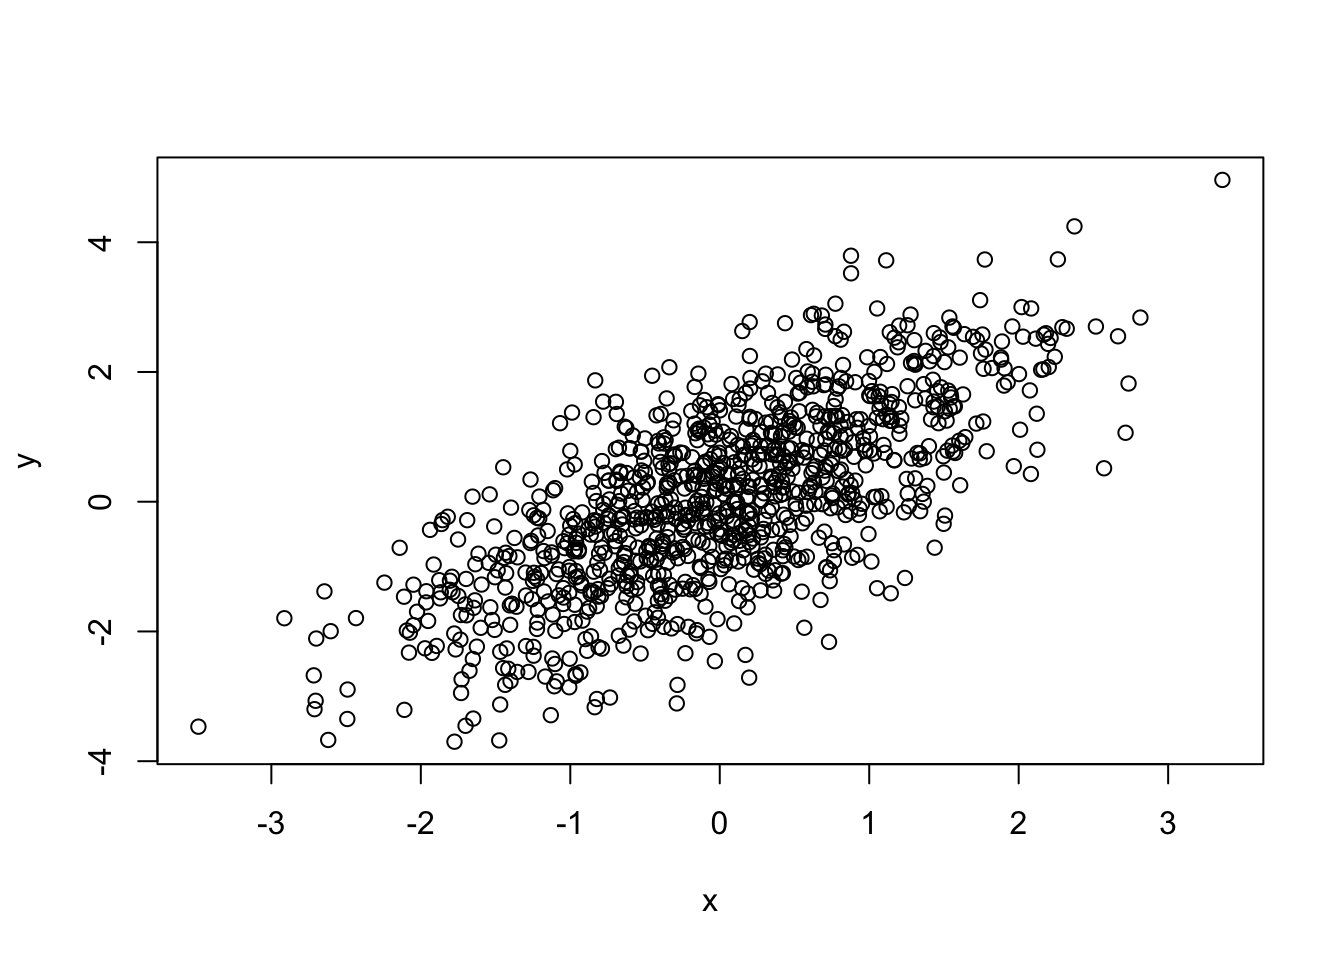
\includegraphics{_main_files/figure-latex/related-variables-1.pdf}

Convenient to manipulate them together

\begin{itemize}
\item
  \texttt{data.frame()}: like columns in a spreadsheet

\begin{Shaded}
\begin{Highlighting}[]
\NormalTok{df =}\StringTok{ }\KeywordTok{data.frame}\NormalTok{(}\DataTypeTok{X=}\NormalTok{x, }\DataTypeTok{Y=}\NormalTok{y)}
\KeywordTok{head}\NormalTok{(df)           }\CommentTok{# first 6 rows}
\end{Highlighting}
\end{Shaded}

\begin{verbatim}
##             X          Y
## 1 -0.72437726 -0.1684765
## 2  0.40709567  0.4559514
## 3 -0.44450808 -0.1445829
## 4 -0.15238336  1.5561891
## 5 -0.03677902  0.3178355
## 6  0.99614929  0.3245457
\end{verbatim}

\begin{Shaded}
\begin{Highlighting}[]
\KeywordTok{plot}\NormalTok{(Y }\OperatorTok{~}\StringTok{ }\NormalTok{X, df)    }\CommentTok{# same as above}
\end{Highlighting}
\end{Shaded}

  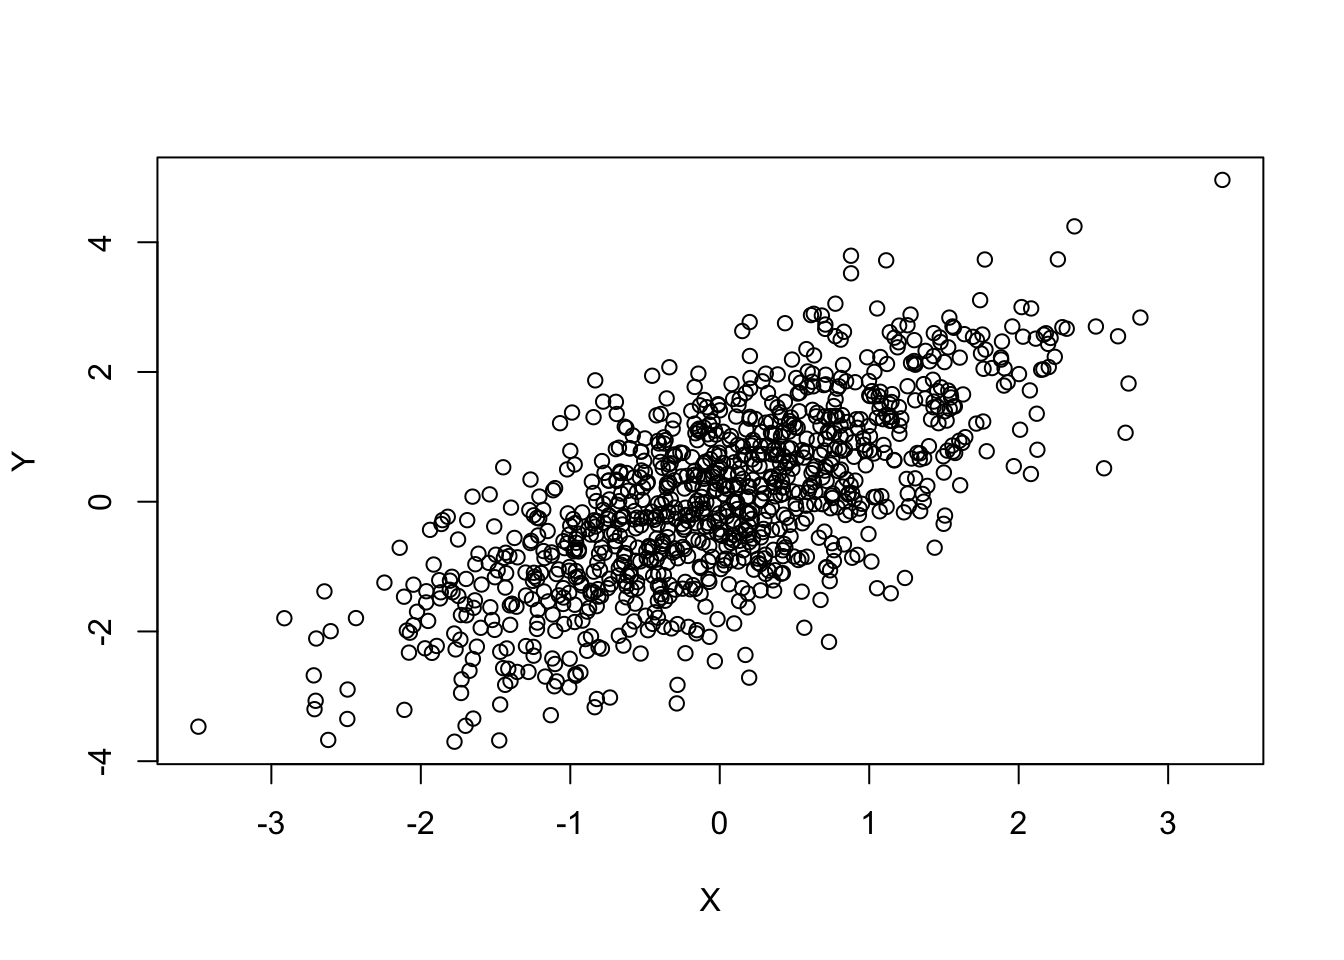
\includegraphics{_main_files/figure-latex/data.frame-1.pdf}
\item
  See all data with \texttt{View(df)}. Summarize data with
  \texttt{summary(df)}

\begin{Shaded}
\begin{Highlighting}[]
\KeywordTok{summary}\NormalTok{(df)}
\end{Highlighting}
\end{Shaded}

\begin{verbatim}
##        X                    Y            
##  Min.   :-2.8326987   Min.   :-4.444125  
##  1st Qu.:-0.6591657   1st Qu.:-0.923660  
##  Median : 0.0003174   Median : 0.043338  
##  Mean   : 0.0398925   Mean   : 0.006076  
##  3rd Qu.: 0.7176888   3rd Qu.: 0.925764  
##  Max.   : 2.9001701   Max.   : 4.235091
\end{verbatim}
\item
  Easy to manipulate data in a coordinated way, e.g., access column
  \texttt{X} with \texttt{\$} and subset for just those values greater
  than 0

\begin{Shaded}
\begin{Highlighting}[]
\NormalTok{positiveX =}\StringTok{ }\NormalTok{df[df}\OperatorTok{$}\NormalTok{X }\OperatorTok{>}\StringTok{ }\DecValTok{0}\NormalTok{,]}
\KeywordTok{head}\NormalTok{(positiveX)}
\end{Highlighting}
\end{Shaded}

\begin{verbatim}
##            X           Y
## 2  0.4070957  0.45595139
## 6  0.9961493  0.32454569
## 8  0.4530330  0.63267547
## 11 0.2187124  0.84211192
## 12 0.2648313 -0.10204721
## 20 0.5874987 -0.08449245
\end{verbatim}

\begin{Shaded}
\begin{Highlighting}[]
\KeywordTok{plot}\NormalTok{(Y }\OperatorTok{~}\StringTok{ }\NormalTok{X, positiveX)}
\end{Highlighting}
\end{Shaded}

  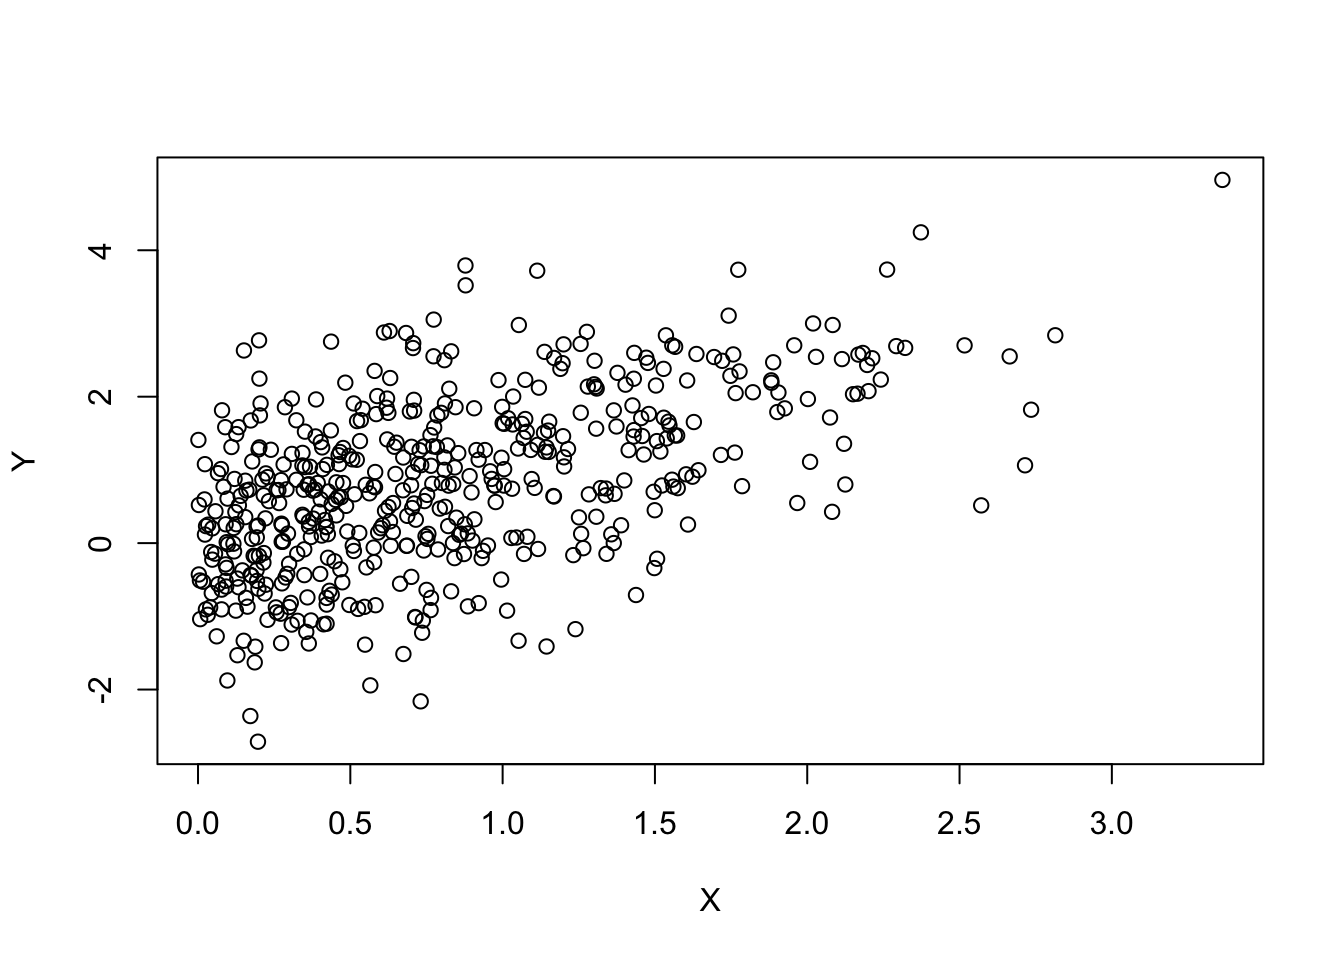
\includegraphics{_main_files/figure-latex/data.frame-subset-1.pdf}
\item
  \emph{R} is introspective -- ask it about itself

\begin{Shaded}
\begin{Highlighting}[]
\KeywordTok{class}\NormalTok{(df)}
\end{Highlighting}
\end{Shaded}

\begin{verbatim}
## [1] "data.frame"
\end{verbatim}

\begin{Shaded}
\begin{Highlighting}[]
\KeywordTok{dim}\NormalTok{(df)}
\end{Highlighting}
\end{Shaded}

\begin{verbatim}
## [1] 1000    2
\end{verbatim}

\begin{Shaded}
\begin{Highlighting}[]
\KeywordTok{colnames}\NormalTok{(df)}
\end{Highlighting}
\end{Shaded}

\begin{verbatim}
## [1] "X" "Y"
\end{verbatim}
\item
  \texttt{matrix()} a related class, where all elements have the same
  type (a \texttt{data.frame()} requires elements within a column to be
  the same type, but elements between columns can be different types).
\end{itemize}

A scatterplot makes one want to fit a linear model (do a regression
analysis)

\begin{itemize}
\item
  Use a \emph{formula} to describe the relationship between variables
\item
  Variables found in the second argument

\begin{Shaded}
\begin{Highlighting}[]
\NormalTok{fit <-}\StringTok{ }\KeywordTok{lm}\NormalTok{(Y }\OperatorTok{~}\StringTok{ }\NormalTok{X, df)}
\end{Highlighting}
\end{Shaded}
\item
  Visualize the points, and add the regression line

\begin{Shaded}
\begin{Highlighting}[]
\KeywordTok{plot}\NormalTok{(Y }\OperatorTok{~}\StringTok{ }\NormalTok{X, df)}
\KeywordTok{abline}\NormalTok{(fit, }\DataTypeTok{col=}\StringTok{"red"}\NormalTok{, }\DataTypeTok{lwd=}\DecValTok{3}\NormalTok{)}
\end{Highlighting}
\end{Shaded}

  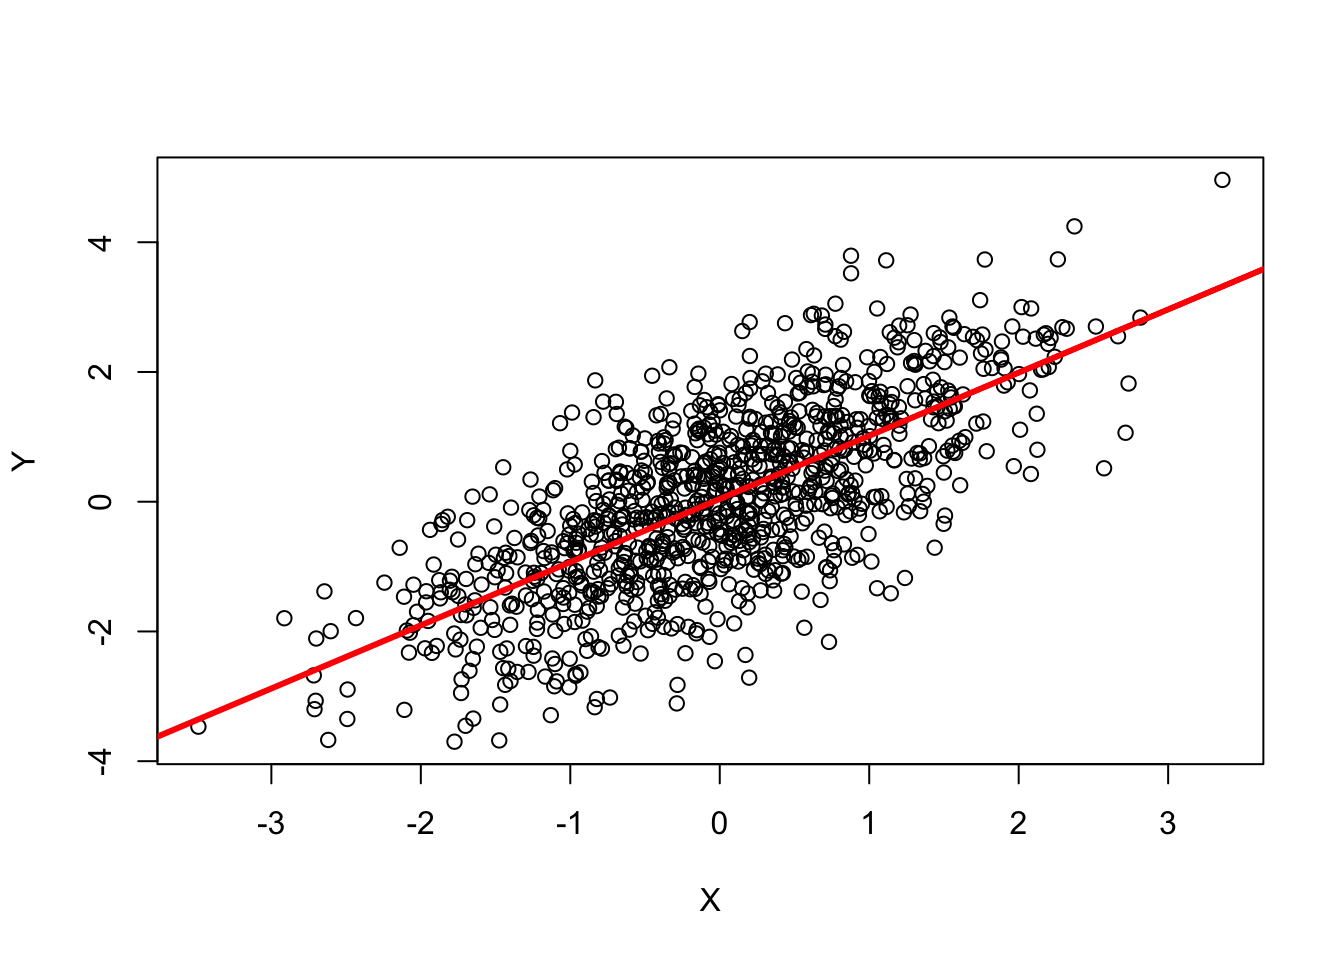
\includegraphics{_main_files/figure-latex/lm-plot-1.pdf}
\item
  Summarize the fit as an ANOVA table

\begin{Shaded}
\begin{Highlighting}[]
\KeywordTok{anova}\NormalTok{(fit)}
\end{Highlighting}
\end{Shaded}

\begin{verbatim}
## Analysis of Variance Table
## 
## Response: Y
##            Df  Sum Sq Mean Sq F value    Pr(>F)    
## X           1  979.93  979.93  966.61 < 2.2e-16 ***
## Residuals 998 1011.76    1.01                      
## ---
## Signif. codes:  0 '***' 0.001 '**' 0.01 '*' 0.05 '.' 0.1 ' ' 1
\end{verbatim}
\item
  N.B. -- `Type I' sums-of-squares, so order of independent variables
  matters; use \texttt{drop1()} for `Type III'. See
  \href{http://www.statmethods.net/stats/anova.html}{DataCamp Quick-R}
\item
  Introspection -- what class is \texttt{fit}? What \emph{methods} can I
  apply to an object of that class?

\begin{Shaded}
\begin{Highlighting}[]
\KeywordTok{class}\NormalTok{(fit)}
\end{Highlighting}
\end{Shaded}

\begin{verbatim}
## [1] "lm"
\end{verbatim}

\begin{Shaded}
\begin{Highlighting}[]
\KeywordTok{methods}\NormalTok{(}\DataTypeTok{class=}\KeywordTok{class}\NormalTok{(fit))}
\end{Highlighting}
\end{Shaded}

\begin{verbatim}
##  [1] add1           alias          anova          case.names    
##  [5] coerce         confint        cooks.distance deviance      
##  [9] dfbeta         dfbetas        drop1          dummy.coef    
## [13] effects        extractAIC     family         formula       
## [17] hatvalues      influence      initialize     kappa         
## [21] labels         logLik         model.frame    model.matrix  
## [25] nobs           plot           predict        print         
## [29] proj           qr             residuals      rstandard     
## [33] rstudent       show           simulate       slotsFromS3   
## [37] summary        variable.names vcov          
## see '?methods' for accessing help and source code
\end{verbatim}
\end{itemize}

\subsection{Help!}\label{help}

Help available in \emph{Rstudio} or interactively

\begin{itemize}
\item
  Check out the help page for \texttt{rnorm()}

\begin{Shaded}
\begin{Highlighting}[]
\NormalTok{?rnorm}
\end{Highlighting}
\end{Shaded}
\item
  `Usage' section describes how the function can be used

\begin{verbatim}
rnorm(n, mean = 0, sd = 1)
\end{verbatim}
\item
  Arguments, some with default values. Arguments matched first by name,
  then position
\item
  `Arguments' section describes what the arguments are supposed to be
\item
  `Value' section describes return value
\item
  `Examples' section illustrates use
\item
  Often include citations to relevant technical documentation, reference
  to related functions, obscure details
\item
  Can be intimidating, but in the end actually \emph{very} useful
\end{itemize}

\section{Exercise 1: BRFSS Survey
Data}\label{exercise-1-brfss-survey-data}

We will explore a subset of data collected by the CDC through its
extensive Behavioral Risk Factor Surveillance System
(\href{http://www.cdc.gov/brfss/about/index.htm}{BRFSS}) telephone
survey. Check out the link for more information. We'll look at a subset
of the data.

\begin{enumerate}
\def\labelenumi{\arabic{enumi}.}
\item
  Use \texttt{file.choose()} to find the path to the file
  `BRFSS-subset.csv'

\begin{Shaded}
\begin{Highlighting}[]
\NormalTok{path <-}\StringTok{ }\KeywordTok{file.choose}\NormalTok{()}
\end{Highlighting}
\end{Shaded}
\end{enumerate}

\begin{enumerate}
\def\labelenumi{\arabic{enumi}.}
\setcounter{enumi}{1}
\item
  Input the data using \texttt{read.csv()}, assigning to a variable
  \texttt{brfss}

\begin{Shaded}
\begin{Highlighting}[]
\NormalTok{brfss <-}\StringTok{ }\KeywordTok{read.csv}\NormalTok{(path)}
\end{Highlighting}
\end{Shaded}
\item
  Use command like \texttt{class()}, \texttt{head()}, \texttt{dim()},
  \texttt{summary()} to explore the data.

  \begin{itemize}
  \item
    What variables have been measured?
  \item
    Can you guess at the units used for, e.g., Weight and Height?
  \end{itemize}

\begin{verbatim}
class(brfss)
head(brfss)
dim(brfss)
summary(brfss)
\end{verbatim}
\item
  Use the \texttt{\$} operator to extract the `Sex' column, and
  summarize the number of males and females in the survey using
  \texttt{table()}. Do the same for `Year', and for both \texttt{Sex}
  and \texttt{Year}

\begin{Shaded}
\begin{Highlighting}[]
\KeywordTok{table}\NormalTok{(brfss}\OperatorTok{$}\NormalTok{Sex)}
\end{Highlighting}
\end{Shaded}

\begin{verbatim}
## 
## Female   Male 
##  12039   7961
\end{verbatim}

\begin{Shaded}
\begin{Highlighting}[]
\KeywordTok{table}\NormalTok{(brfss}\OperatorTok{$}\NormalTok{Year)}
\end{Highlighting}
\end{Shaded}

\begin{verbatim}
## 
##  1990  2010 
## 10000 10000
\end{verbatim}

\begin{Shaded}
\begin{Highlighting}[]
\KeywordTok{table}\NormalTok{(brfss}\OperatorTok{$}\NormalTok{Sex, brfss}\OperatorTok{$}\NormalTok{Year)}
\end{Highlighting}
\end{Shaded}

\begin{verbatim}
##         
##          1990 2010
##   Female 5718 6321
##   Male   4282 3679
\end{verbatim}

\begin{Shaded}
\begin{Highlighting}[]
\KeywordTok{with}\NormalTok{(brfss, }\KeywordTok{table}\NormalTok{(Sex, Year))                }\CommentTok{# same, but easier}
\end{Highlighting}
\end{Shaded}

\begin{verbatim}
##         Year
## Sex      1990 2010
##   Female 5718 6321
##   Male   4282 3679
\end{verbatim}
\item
  Use \texttt{aggregate()} to summarize the mean weight of each group.
  What about the median weight of each group? What about the
  \emph{number} of observations in each group?

\begin{Shaded}
\begin{Highlighting}[]
\KeywordTok{with}\NormalTok{(brfss, }\KeywordTok{aggregate}\NormalTok{(Weight, }\KeywordTok{list}\NormalTok{(Year, Sex), mean, }\DataTypeTok{na.rm=}\OtherTok{TRUE}\NormalTok{))}
\end{Highlighting}
\end{Shaded}

\begin{verbatim}
##   Group.1 Group.2        x
## 1    1990  Female 64.81838
## 2    2010  Female 72.95424
## 3    1990    Male 81.17999
## 4    2010    Male 88.84657
\end{verbatim}

\begin{Shaded}
\begin{Highlighting}[]
\KeywordTok{with}\NormalTok{(brfss, }\KeywordTok{aggregate}\NormalTok{(Weight, }\KeywordTok{list}\NormalTok{(}\DataTypeTok{Year=}\NormalTok{Year, }\DataTypeTok{Sex=}\NormalTok{Sex), mean, }\DataTypeTok{na.rm=}\OtherTok{TRUE}\NormalTok{))}
\end{Highlighting}
\end{Shaded}

\begin{verbatim}
##   Year    Sex        x
## 1 1990 Female 64.81838
## 2 2010 Female 72.95424
## 3 1990   Male 81.17999
## 4 2010   Male 88.84657
\end{verbatim}
\item
  Use a \texttt{formula} and the \texttt{aggregate()} function to
  describe the relationship between Year, Sex, and Weight

\begin{Shaded}
\begin{Highlighting}[]
\KeywordTok{aggregate}\NormalTok{(Weight }\OperatorTok{~}\StringTok{ }\NormalTok{Year }\OperatorTok{+}\StringTok{ }\NormalTok{Sex, brfss, mean)  }\CommentTok{# same, but more informative}
\end{Highlighting}
\end{Shaded}

\begin{verbatim}
##   Year    Sex   Weight
## 1 1990 Female 64.81838
## 2 2010 Female 72.95424
## 3 1990   Male 81.17999
## 4 2010   Male 88.84657
\end{verbatim}

\begin{Shaded}
\begin{Highlighting}[]
\KeywordTok{aggregate}\NormalTok{(. }\OperatorTok{~}\StringTok{ }\NormalTok{Year }\OperatorTok{+}\StringTok{ }\NormalTok{Sex, brfss, mean)       }\CommentTok{# all variables}
\end{Highlighting}
\end{Shaded}

\begin{verbatim}
##   Year    Sex      Age   Weight   Height
## 1 1990 Female 46.09153 64.84333 163.2914
## 2 2010 Female 57.07807 73.03178 163.2469
## 3 1990   Male 43.87574 81.19496 178.2242
## 4 2010   Male 56.25465 88.91136 178.0139
\end{verbatim}
\item
  Create a subset of the data consisting of only the 1990 observations.
  Perform a t-test comparing the weight of males and females
  (``\,`Weight' as a function of `Sex'\,'',
  \texttt{Weight\ \textasciitilde{}\ Sex})

\begin{Shaded}
\begin{Highlighting}[]
\NormalTok{brfss_}\DecValTok{1990}\NormalTok{ =}\StringTok{ }\NormalTok{brfss[brfss}\OperatorTok{$}\NormalTok{Year }\OperatorTok{==}\StringTok{ }\DecValTok{1990}\NormalTok{,]}
\KeywordTok{t.test}\NormalTok{(Weight }\OperatorTok{~}\StringTok{ }\NormalTok{Sex, brfss_}\DecValTok{1990}\NormalTok{)}
\end{Highlighting}
\end{Shaded}

\begin{verbatim}
## 
##  Welch Two Sample t-test
## 
## data:  Weight by Sex
## t = -58.734, df = 9214, p-value < 2.2e-16
## alternative hypothesis: true difference in means is not equal to 0
## 95 percent confidence interval:
##  -16.90767 -15.81554
## sample estimates:
## mean in group Female   mean in group Male 
##             64.81838             81.17999
\end{verbatim}

\begin{Shaded}
\begin{Highlighting}[]
\KeywordTok{t.test}\NormalTok{(Weight }\OperatorTok{~}\StringTok{ }\NormalTok{Sex, brfss, }\DataTypeTok{subset =}\NormalTok{ Year }\OperatorTok{==}\StringTok{ }\DecValTok{1990}\NormalTok{)}
\end{Highlighting}
\end{Shaded}

\begin{verbatim}
## 
##  Welch Two Sample t-test
## 
## data:  Weight by Sex
## t = -58.734, df = 9214, p-value < 2.2e-16
## alternative hypothesis: true difference in means is not equal to 0
## 95 percent confidence interval:
##  -16.90767 -15.81554
## sample estimates:
## mean in group Female   mean in group Male 
##             64.81838             81.17999
\end{verbatim}

  What about differences between weights of males (or females) in 1990
  versus 2010? Check out the help page \texttt{?t.test.formula}. Is
  there a way of performing a t-test on \texttt{brfss} without
  explicitly creating the object \texttt{brfss\_1990}?
\item
  Use \texttt{boxplot()} to plot the weights of the Male individuals.
  Can you transform weight, e.g.,
  \texttt{sqrt(Weight)\ \textasciitilde{}\ Year}? Interpret the results.
  Do similar boxplots for the t-tests of the previous question.

\begin{Shaded}
\begin{Highlighting}[]
\KeywordTok{boxplot}\NormalTok{(Weight }\OperatorTok{~}\StringTok{ }\NormalTok{Year, brfss, }\DataTypeTok{subset =}\NormalTok{ Sex }\OperatorTok{==}\StringTok{ "Male"}\NormalTok{,}
        \DataTypeTok{main=}\StringTok{"Males"}\NormalTok{)}
\end{Highlighting}
\end{Shaded}

  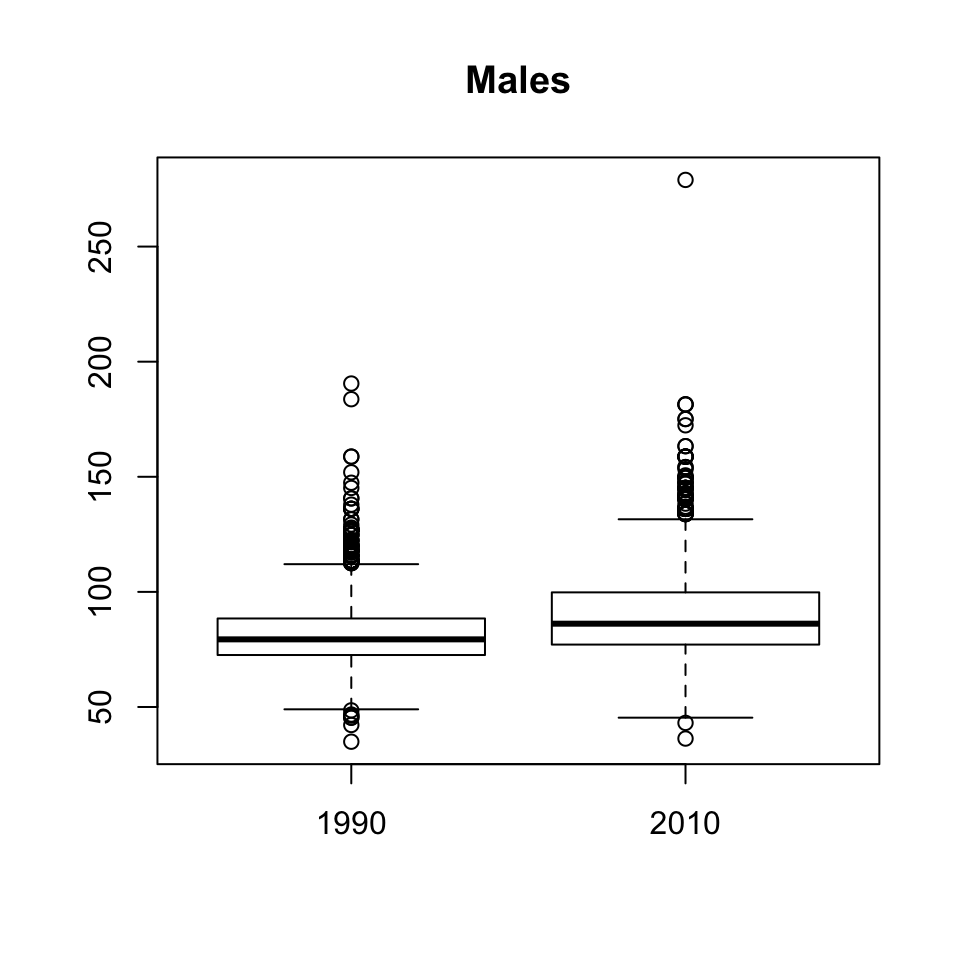
\includegraphics{_main_files/figure-latex/brfss-boxplot-1.pdf}
\item
  Use \texttt{hist()} to plot a histogram of weights of the 1990 Female
  individuals.

\begin{Shaded}
\begin{Highlighting}[]
\KeywordTok{hist}\NormalTok{(brfss_}\DecValTok{1990}\NormalTok{[brfss_}\DecValTok{1990}\OperatorTok{$}\NormalTok{Sex }\OperatorTok{==}\StringTok{ "Female"}\NormalTok{, }\StringTok{"Weight"}\NormalTok{],}
     \DataTypeTok{main=}\StringTok{"Females, 1990"}\NormalTok{, }\DataTypeTok{xlab=}\StringTok{"Weight"}\NormalTok{ )}
\end{Highlighting}
\end{Shaded}

  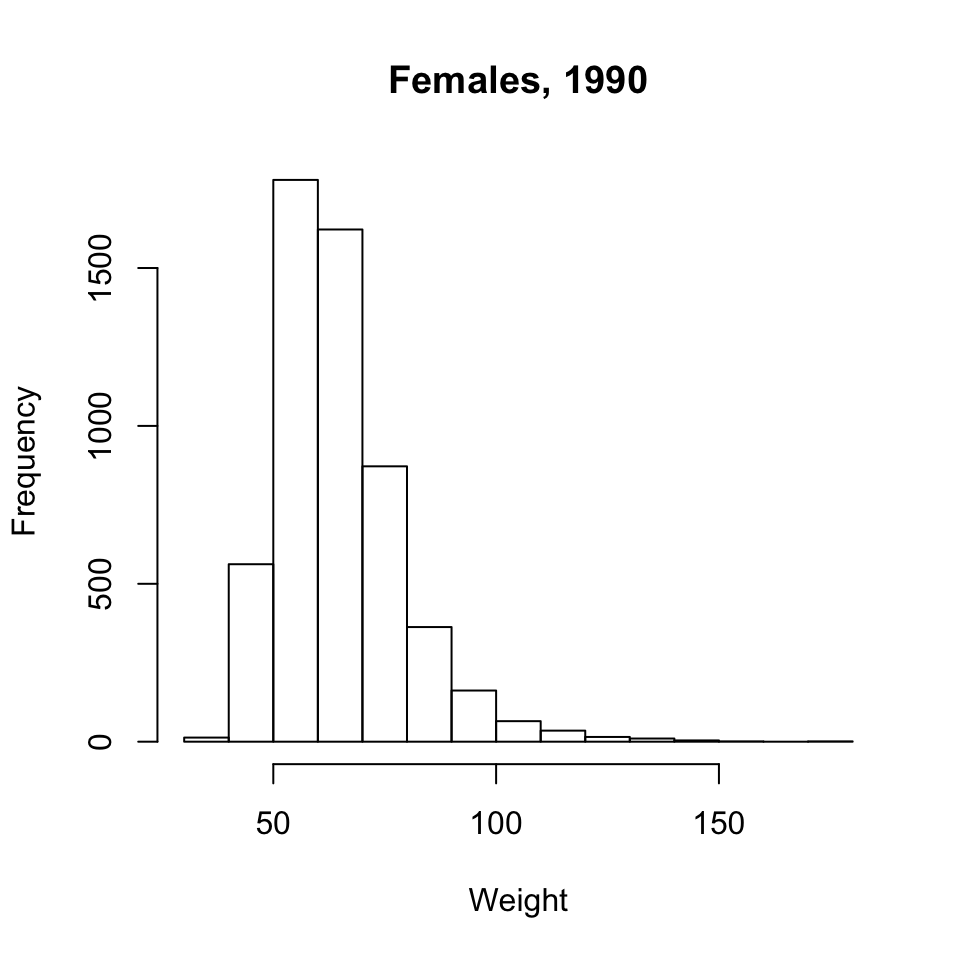
\includegraphics{_main_files/figure-latex/brfss-hist-1.pdf}
\end{enumerate}

\section{Exercise 2: ALL Phenotypic
Data}\label{exercise-2-all-phenotypic-data}

This data comes from an (old) Acute Lymphoid Leukemia microarray data
set.

Choose the file that contains ALL (acute lymphoblastic leukemia) patient
information and input the date using \texttt{read.csv()}; for
\texttt{read.csv()}, use \texttt{row.names=1} to indicate that the first
column contains row names.

\begin{Shaded}
\begin{Highlighting}[]
\NormalTok{path <-}\StringTok{ }\KeywordTok{file.choose}\NormalTok{()    }\CommentTok{# look for ALL-phenoData.csv}
\end{Highlighting}
\end{Shaded}

\begin{Shaded}
\begin{Highlighting}[]
\KeywordTok{stopifnot}\NormalTok{(}\KeywordTok{file.exists}\NormalTok{(path))}
\NormalTok{pdata <-}\StringTok{ }\KeywordTok{read.csv}\NormalTok{(path, }\DataTypeTok{row.names=}\DecValTok{1}\NormalTok{)}
\end{Highlighting}
\end{Shaded}

Check out the help page \texttt{?read.delim} for input options. The
exercises use \texttt{?read.csv}; Can you guess why? Explore basic
properties of the object you've created, for instance\ldots{}

\begin{Shaded}
\begin{Highlighting}[]
\KeywordTok{class}\NormalTok{(pdata)}
\end{Highlighting}
\end{Shaded}

\begin{verbatim}
## [1] "data.frame"
\end{verbatim}

\begin{Shaded}
\begin{Highlighting}[]
\KeywordTok{colnames}\NormalTok{(pdata)}
\end{Highlighting}
\end{Shaded}

\begin{verbatim}
##  [1] "cod"            "diagnosis"      "sex"            "age"           
##  [5] "BT"             "remission"      "CR"             "date.cr"       
##  [9] "t.4.11."        "t.9.22."        "cyto.normal"    "citog"         
## [13] "mol.biol"       "fusion.protein" "mdr"            "kinet"         
## [17] "ccr"            "relapse"        "transplant"     "f.u"           
## [21] "date.last.seen"
\end{verbatim}

\begin{Shaded}
\begin{Highlighting}[]
\KeywordTok{dim}\NormalTok{(pdata)}
\end{Highlighting}
\end{Shaded}

\begin{verbatim}
## [1] 128  21
\end{verbatim}

\begin{Shaded}
\begin{Highlighting}[]
\KeywordTok{head}\NormalTok{(pdata)}
\end{Highlighting}
\end{Shaded}

\begin{verbatim}
##        cod diagnosis sex age BT remission CR   date.cr t.4.11. t.9.22.
## 01005 1005 5/21/1997   M  53 B2        CR CR  8/6/1997   FALSE    TRUE
## 01010 1010 3/29/2000   M  19 B2        CR CR 6/27/2000   FALSE   FALSE
## 03002 3002 6/24/1998   F  52 B4        CR CR 8/17/1998      NA      NA
## 04006 4006 7/17/1997   M  38 B1        CR CR  9/8/1997    TRUE   FALSE
## 04007 4007 7/22/1997   M  57 B2        CR CR 9/17/1997   FALSE   FALSE
## 04008 4008 7/30/1997   M  17 B1        CR CR 9/27/1997   FALSE   FALSE
##       cyto.normal        citog mol.biol fusion.protein mdr   kinet   ccr
## 01005       FALSE      t(9;22)  BCR/ABL           p210 NEG dyploid FALSE
## 01010       FALSE  simple alt.      NEG           <NA> POS dyploid FALSE
## 03002          NA         <NA>  BCR/ABL           p190 NEG dyploid FALSE
## 04006       FALSE      t(4;11) ALL1/AF4           <NA> NEG dyploid FALSE
## 04007       FALSE      del(6q)      NEG           <NA> NEG dyploid FALSE
## 04008       FALSE complex alt.      NEG           <NA> NEG hyperd. FALSE
##       relapse transplant               f.u date.last.seen
## 01005   FALSE       TRUE BMT / DEATH IN CR           <NA>
## 01010    TRUE      FALSE               REL      8/28/2000
## 03002    TRUE      FALSE               REL     10/15/1999
## 04006    TRUE      FALSE               REL      1/23/1998
## 04007    TRUE      FALSE               REL      11/4/1997
## 04008    TRUE      FALSE               REL     12/15/1997
\end{verbatim}

\begin{Shaded}
\begin{Highlighting}[]
\KeywordTok{summary}\NormalTok{(pdata}\OperatorTok{$}\NormalTok{sex)}
\end{Highlighting}
\end{Shaded}

\begin{verbatim}
##    F    M NA's 
##   42   83    3
\end{verbatim}

\begin{Shaded}
\begin{Highlighting}[]
\KeywordTok{summary}\NormalTok{(pdata}\OperatorTok{$}\NormalTok{cyto.normal)}
\end{Highlighting}
\end{Shaded}

\begin{verbatim}
##    Mode   FALSE    TRUE    NA's 
## logical      69      24      35
\end{verbatim}

Remind yourselves about various ways to subset and access columns of a
data.frame

\begin{Shaded}
\begin{Highlighting}[]
\NormalTok{pdata[}\DecValTok{1}\OperatorTok{:}\DecValTok{5}\NormalTok{, }\DecValTok{3}\OperatorTok{:}\DecValTok{4}\NormalTok{]}
\end{Highlighting}
\end{Shaded}

\begin{verbatim}
##       sex age
## 01005   M  53
## 01010   M  19
## 03002   F  52
## 04006   M  38
## 04007   M  57
\end{verbatim}

\begin{Shaded}
\begin{Highlighting}[]
\NormalTok{pdata[}\DecValTok{1}\OperatorTok{:}\DecValTok{5}\NormalTok{, ]}
\end{Highlighting}
\end{Shaded}

\begin{verbatim}
##        cod diagnosis sex age BT remission CR   date.cr t.4.11. t.9.22.
## 01005 1005 5/21/1997   M  53 B2        CR CR  8/6/1997   FALSE    TRUE
## 01010 1010 3/29/2000   M  19 B2        CR CR 6/27/2000   FALSE   FALSE
## 03002 3002 6/24/1998   F  52 B4        CR CR 8/17/1998      NA      NA
## 04006 4006 7/17/1997   M  38 B1        CR CR  9/8/1997    TRUE   FALSE
## 04007 4007 7/22/1997   M  57 B2        CR CR 9/17/1997   FALSE   FALSE
##       cyto.normal       citog mol.biol fusion.protein mdr   kinet   ccr
## 01005       FALSE     t(9;22)  BCR/ABL           p210 NEG dyploid FALSE
## 01010       FALSE simple alt.      NEG           <NA> POS dyploid FALSE
## 03002          NA        <NA>  BCR/ABL           p190 NEG dyploid FALSE
## 04006       FALSE     t(4;11) ALL1/AF4           <NA> NEG dyploid FALSE
## 04007       FALSE     del(6q)      NEG           <NA> NEG dyploid FALSE
##       relapse transplant               f.u date.last.seen
## 01005   FALSE       TRUE BMT / DEATH IN CR           <NA>
## 01010    TRUE      FALSE               REL      8/28/2000
## 03002    TRUE      FALSE               REL     10/15/1999
## 04006    TRUE      FALSE               REL      1/23/1998
## 04007    TRUE      FALSE               REL      11/4/1997
\end{verbatim}

\begin{Shaded}
\begin{Highlighting}[]
\KeywordTok{head}\NormalTok{(pdata[, }\DecValTok{3}\OperatorTok{:}\DecValTok{5}\NormalTok{])}
\end{Highlighting}
\end{Shaded}

\begin{verbatim}
##       sex age BT
## 01005   M  53 B2
## 01010   M  19 B2
## 03002   F  52 B4
## 04006   M  38 B1
## 04007   M  57 B2
## 04008   M  17 B1
\end{verbatim}

\begin{Shaded}
\begin{Highlighting}[]
\KeywordTok{tail}\NormalTok{(pdata[, }\DecValTok{3}\OperatorTok{:}\DecValTok{5}\NormalTok{], }\DecValTok{3}\NormalTok{)}
\end{Highlighting}
\end{Shaded}

\begin{verbatim}
##        sex age BT
## 65003    M  30 T3
## 83001    M  29 T2
## LAL4  <NA>  NA  T
\end{verbatim}

\begin{Shaded}
\begin{Highlighting}[]
\KeywordTok{head}\NormalTok{(pdata}\OperatorTok{$}\NormalTok{age)}
\end{Highlighting}
\end{Shaded}

\begin{verbatim}
## [1] 53 19 52 38 57 17
\end{verbatim}

\begin{Shaded}
\begin{Highlighting}[]
\KeywordTok{head}\NormalTok{(pdata}\OperatorTok{$}\NormalTok{sex)}
\end{Highlighting}
\end{Shaded}

\begin{verbatim}
## [1] M M F M M M
## Levels: F M
\end{verbatim}

\begin{Shaded}
\begin{Highlighting}[]
\KeywordTok{head}\NormalTok{(pdata[pdata}\OperatorTok{$}\NormalTok{age }\OperatorTok{>}\StringTok{ }\DecValTok{21}\NormalTok{,])}
\end{Highlighting}
\end{Shaded}

\begin{verbatim}
##        cod diagnosis sex age BT remission CR   date.cr t.4.11. t.9.22.
## 01005 1005 5/21/1997   M  53 B2        CR CR  8/6/1997   FALSE    TRUE
## 03002 3002 6/24/1998   F  52 B4        CR CR 8/17/1998      NA      NA
## 04006 4006 7/17/1997   M  38 B1        CR CR  9/8/1997    TRUE   FALSE
## 04007 4007 7/22/1997   M  57 B2        CR CR 9/17/1997   FALSE   FALSE
## 08001 8001 1/15/1997   M  40 B2        CR CR 3/26/1997   FALSE   FALSE
## 08011 8011 8/21/1998   M  33 B3        CR CR 10/8/1998   FALSE   FALSE
##       cyto.normal        citog mol.biol fusion.protein mdr   kinet   ccr
## 01005       FALSE      t(9;22)  BCR/ABL           p210 NEG dyploid FALSE
## 03002          NA         <NA>  BCR/ABL           p190 NEG dyploid FALSE
## 04006       FALSE      t(4;11) ALL1/AF4           <NA> NEG dyploid FALSE
## 04007       FALSE      del(6q)      NEG           <NA> NEG dyploid FALSE
## 08001       FALSE     del(p15)  BCR/ABL           p190 NEG    <NA> FALSE
## 08011       FALSE del(p15/p16)  BCR/ABL      p190/p210 NEG dyploid FALSE
##       relapse transplant               f.u date.last.seen
## 01005   FALSE       TRUE BMT / DEATH IN CR           <NA>
## 03002    TRUE      FALSE               REL     10/15/1999
## 04006    TRUE      FALSE               REL      1/23/1998
## 04007    TRUE      FALSE               REL      11/4/1997
## 08001    TRUE      FALSE               REL      7/11/1997
## 08011   FALSE       TRUE BMT / DEATH IN CR           <NA>
\end{verbatim}

It seems from below that there are 17 females over 40 in the data set.
However, some individuals have \texttt{NA} for the age and / or sex, and
these \texttt{NA} values propagate through some computations. Use
\texttt{table()} to summarize the number of females over 40, and the
number of samples for which this classification cannot be determined.
When \emph{R} encounters an \texttt{NA} value in a subscript index, it
introduces an \texttt{NA} into the result. Observe this (rows of
\texttt{NA} values introduced into the result) when subsetting using
\texttt{{[}} versus using the \texttt{subset()} function.

\begin{Shaded}
\begin{Highlighting}[]
\NormalTok{idx <-}\StringTok{ }\NormalTok{pdata}\OperatorTok{$}\NormalTok{sex }\OperatorTok{==}\StringTok{ "F"} \OperatorTok{&}\StringTok{ }\NormalTok{pdata}\OperatorTok{$}\NormalTok{age }\OperatorTok{>}\StringTok{ }\DecValTok{40}
\KeywordTok{table}\NormalTok{(idx, }\DataTypeTok{useNA=}\StringTok{"ifany"}\NormalTok{)}
\end{Highlighting}
\end{Shaded}

\begin{verbatim}
## idx
## FALSE  TRUE  <NA> 
##   108    17     3
\end{verbatim}

\begin{Shaded}
\begin{Highlighting}[]
\KeywordTok{dim}\NormalTok{(pdata[idx,])           }\CommentTok{# }\AlertTok{WARNING}\CommentTok{: 'NA' rows introduced}
\end{Highlighting}
\end{Shaded}

\begin{verbatim}
## [1] 20 21
\end{verbatim}

\begin{Shaded}
\begin{Highlighting}[]
\KeywordTok{tail}\NormalTok{(pdata[idx,])}
\end{Highlighting}
\end{Shaded}

\begin{verbatim}
##         cod  diagnosis  sex age   BT remission                 CR
## 49006 49006  8/12/1998    F  43   B2        CR                 CR
## 57001 57001  1/29/1997    F  53   B3      <NA> DEATH IN INDUCTION
## 62001 62001 11/11/1997    F  50   B4       REF                REF
## NA.1   <NA>       <NA> <NA>  NA <NA>      <NA>               <NA>
## 02020  2020  3/23/2000    F  48   T2      <NA> DEATH IN INDUCTION
## NA.2   <NA>       <NA> <NA>  NA <NA>      <NA>               <NA>
##          date.cr t.4.11. t.9.22. cyto.normal         citog mol.biol
## 49006 11/19/1998      NA      NA          NA          <NA>  BCR/ABL
## 57001       <NA>   FALSE   FALSE        TRUE        normal      NEG
## 62001       <NA>   FALSE    TRUE       FALSE t(9;22)+other  BCR/ABL
## NA.1        <NA>      NA      NA          NA          <NA>     <NA>
## 02020       <NA>   FALSE   FALSE       FALSE  complex alt.      NEG
## NA.2        <NA>      NA      NA          NA          <NA>     <NA>
##       fusion.protein  mdr   kinet   ccr relapse transplant  f.u
## 49006           p210  NEG dyploid FALSE    TRUE      FALSE  REL
## 57001           <NA>  NEG hyperd.    NA      NA         NA <NA>
## 62001           <NA>  NEG hyperd.    NA      NA         NA <NA>
## NA.1            <NA> <NA>    <NA>    NA      NA         NA <NA>
## 02020           <NA>  NEG dyploid    NA      NA         NA <NA>
## NA.2            <NA> <NA>    <NA>    NA      NA         NA <NA>
##       date.last.seen
## 49006      4/26/1999
## 57001           <NA>
## 62001           <NA>
## NA.1            <NA>
## 02020           <NA>
## NA.2            <NA>
\end{verbatim}

\begin{Shaded}
\begin{Highlighting}[]
\KeywordTok{dim}\NormalTok{(}\KeywordTok{subset}\NormalTok{(pdata, idx))    }\CommentTok{# BETTER: no NA rows}
\end{Highlighting}
\end{Shaded}

\begin{verbatim}
## [1] 17 21
\end{verbatim}

\begin{Shaded}
\begin{Highlighting}[]
\KeywordTok{dim}\NormalTok{(}\KeywordTok{subset}\NormalTok{(pdata, (sex }\OperatorTok{==}\StringTok{ "F"}\NormalTok{) }\OperatorTok{&}\StringTok{ }\NormalTok{(age }\OperatorTok{>}\StringTok{ }\DecValTok{40}\NormalTok{)))  }\CommentTok{# alternative}
\end{Highlighting}
\end{Shaded}

\begin{verbatim}
## [1] 17 21
\end{verbatim}

\begin{Shaded}
\begin{Highlighting}[]
\KeywordTok{tail}\NormalTok{(}\KeywordTok{subset}\NormalTok{(pdata,idx))}
\end{Highlighting}
\end{Shaded}

\begin{verbatim}
##         cod  diagnosis sex age BT remission                 CR    date.cr
## 28032 28032  9/26/1998   F  52 B1        CR                 CR 10/30/1998
## 30001 30001  1/16/1997   F  54 B3      <NA> DEATH IN INDUCTION       <NA>
## 49006 49006  8/12/1998   F  43 B2        CR                 CR 11/19/1998
## 57001 57001  1/29/1997   F  53 B3      <NA> DEATH IN INDUCTION       <NA>
## 62001 62001 11/11/1997   F  50 B4       REF                REF       <NA>
## 02020  2020  3/23/2000   F  48 T2      <NA> DEATH IN INDUCTION       <NA>
##       t.4.11. t.9.22. cyto.normal         citog mol.biol fusion.protein
## 28032    TRUE   FALSE       FALSE       t(4;11) ALL1/AF4           <NA>
## 30001   FALSE    TRUE       FALSE t(9;22)+other  BCR/ABL           p190
## 49006      NA      NA          NA          <NA>  BCR/ABL           p210
## 57001   FALSE   FALSE        TRUE        normal      NEG           <NA>
## 62001   FALSE    TRUE       FALSE t(9;22)+other  BCR/ABL           <NA>
## 02020   FALSE   FALSE       FALSE  complex alt.      NEG           <NA>
##       mdr   kinet   ccr relapse transplant  f.u date.last.seen
## 28032 NEG dyploid  TRUE   FALSE      FALSE  CCR      5/16/2002
## 30001 NEG hyperd.    NA      NA         NA <NA>           <NA>
## 49006 NEG dyploid FALSE    TRUE      FALSE  REL      4/26/1999
## 57001 NEG hyperd.    NA      NA         NA <NA>           <NA>
## 62001 NEG hyperd.    NA      NA         NA <NA>           <NA>
## 02020 NEG dyploid    NA      NA         NA <NA>           <NA>
\end{verbatim}

\begin{Shaded}
\begin{Highlighting}[]
\NormalTok{## robust `[`: exclude NA values}
\KeywordTok{dim}\NormalTok{(pdata[idx }\OperatorTok{&}\StringTok{ }\OperatorTok{!}\KeywordTok{is.na}\NormalTok{(idx),])}
\end{Highlighting}
\end{Shaded}

\begin{verbatim}
## [1] 17 21
\end{verbatim}

Use the \texttt{mol.biol} column to subset the data to contain just
individuals with `BCR/ABL' or `NEG', e.g.,

\begin{Shaded}
\begin{Highlighting}[]
\NormalTok{bcrabl <-}\StringTok{ }\KeywordTok{subset}\NormalTok{(pdata, mol.biol }\OperatorTok\StringTok{ }\KeywordTok{c}\NormalTok{(}\StringTok{"BCR/ABL"}\NormalTok{, }\StringTok{"NEG"}\NormalTok{))}
\end{Highlighting}
\end{Shaded}

The \texttt{mol.biol} column is a factor, and retains all levels even
after subsetting. It is sometimes convenient to retain factor levels,
but in our case we use \texttt{droplevels()} to removed unused levels

\begin{Shaded}
\begin{Highlighting}[]
\NormalTok{bcrabl}\OperatorTok{$}\NormalTok{mol.biol <-}\StringTok{ }\KeywordTok{droplevels}\NormalTok{(bcrabl}\OperatorTok{$}\NormalTok{mol.biol)}
\end{Highlighting}
\end{Shaded}

The \texttt{BT} column is a factor describing B- and T-cell subtypes

\begin{Shaded}
\begin{Highlighting}[]
\KeywordTok{levels}\NormalTok{(bcrabl}\OperatorTok{$}\NormalTok{BT)}
\end{Highlighting}
\end{Shaded}

\begin{verbatim}
##  [1] "B"  "B1" "B2" "B3" "B4" "T"  "T1" "T2" "T3" "T4"
\end{verbatim}

How might one collapse B1, B2, \ldots{} to a single type B, and likewise
for T1, T2, \ldots{}, so there are only two subtypes, B and T? One
strategy is to replace two-letter level (e.g., \texttt{B1}) with the
single-letter level (e.g., \texttt{B}). Do this using
\texttt{substring()} to select the first letter of level, and update the
previous levels with the new value using \texttt{levels\textless{}-}.

\begin{Shaded}
\begin{Highlighting}[]
\KeywordTok{table}\NormalTok{(bcrabl}\OperatorTok{$}\NormalTok{BT)}
\end{Highlighting}
\end{Shaded}

\begin{verbatim}
## 
##  B B1 B2 B3 B4  T T1 T2 T3 T4 
##  4  9 35 22  9  5  1 15  9  2
\end{verbatim}

\begin{Shaded}
\begin{Highlighting}[]
\KeywordTok{levels}\NormalTok{(bcrabl}\OperatorTok{$}\NormalTok{BT) <-}\StringTok{ }\KeywordTok{substring}\NormalTok{(}\KeywordTok{levels}\NormalTok{(bcrabl}\OperatorTok{$}\NormalTok{BT), }\DecValTok{1}\NormalTok{, }\DecValTok{1}\NormalTok{)}
\KeywordTok{table}\NormalTok{(bcrabl}\OperatorTok{$}\NormalTok{BT)}
\end{Highlighting}
\end{Shaded}

\begin{verbatim}
## 
##  B  T 
## 79 32
\end{verbatim}

Use \texttt{aggregate()} to count the number of samples with B- and
T-cell types in each of the BCR/ABL and NEG groups

\begin{Shaded}
\begin{Highlighting}[]
\KeywordTok{aggregate}\NormalTok{(}\KeywordTok{rownames}\NormalTok{(bcrabl) }\OperatorTok{~}\StringTok{ }\NormalTok{BT }\OperatorTok{+}\StringTok{ }\NormalTok{mol.biol, bcrabl, length)}
\end{Highlighting}
\end{Shaded}

\begin{verbatim}
##   BT mol.biol rownames(bcrabl)
## 1  B  BCR/ABL               37
## 2  B      NEG               42
## 3  T      NEG               32
\end{verbatim}

Use \texttt{aggregate()} to calculate the average age of males and
females in the BCR/ABL and NEG treatment groups.

\begin{Shaded}
\begin{Highlighting}[]
\KeywordTok{aggregate}\NormalTok{(age }\OperatorTok{~}\StringTok{ }\NormalTok{mol.biol }\OperatorTok{+}\StringTok{ }\NormalTok{sex, bcrabl, mean)}
\end{Highlighting}
\end{Shaded}

\begin{verbatim}
##   mol.biol sex      age
## 1  BCR/ABL   F 39.93750
## 2      NEG   F 30.42105
## 3  BCR/ABL   M 40.50000
## 4      NEG   M 27.21154
\end{verbatim}

Use \texttt{t.test()} to compare the age of individuals in the BCR/ABL
versus NEG groups; visualize the results using \texttt{boxplot()}. In
both cases, use the \texttt{formula} interface. Consult the help page
\texttt{?t.test} and re-do the test assuming that variance of ages in
the two groups is identical. What parts of the test output change?

\begin{Shaded}
\begin{Highlighting}[]
\KeywordTok{t.test}\NormalTok{(age }\OperatorTok{~}\StringTok{ }\NormalTok{mol.biol, bcrabl)}
\end{Highlighting}
\end{Shaded}

\begin{verbatim}
## 
##  Welch Two Sample t-test
## 
## data:  age by mol.biol
## t = 4.8172, df = 68.529, p-value = 8.401e-06
## alternative hypothesis: true difference in means is not equal to 0
## 95 percent confidence interval:
##   7.13507 17.22408
## sample estimates:
## mean in group BCR/ABL     mean in group NEG 
##              40.25000              28.07042
\end{verbatim}

\begin{Shaded}
\begin{Highlighting}[]
\KeywordTok{boxplot}\NormalTok{(age }\OperatorTok{~}\StringTok{ }\NormalTok{mol.biol, bcrabl)}
\end{Highlighting}
\end{Shaded}

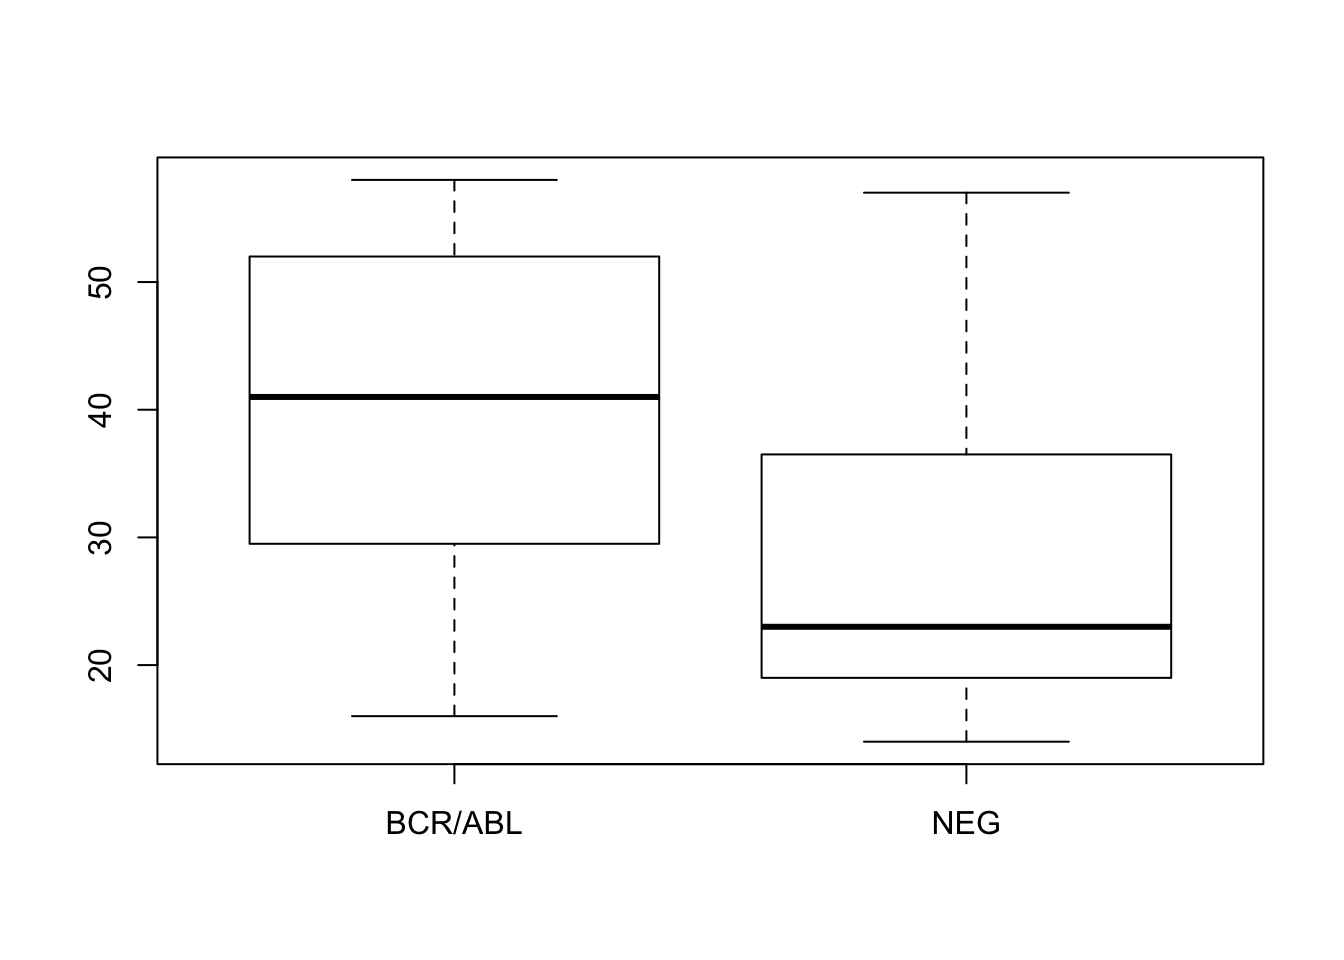
\includegraphics{_main_files/figure-latex/ALL-age-1.pdf}

\section{Exploration and simple univariate
measures}\label{exploration-and-simple-univariate-measures}

\begin{Shaded}
\begin{Highlighting}[]
\NormalTok{path <-}\StringTok{ }\KeywordTok{file.choose}\NormalTok{()    }\CommentTok{# look for BRFSS-subset.csv}
\end{Highlighting}
\end{Shaded}

\begin{Shaded}
\begin{Highlighting}[]
\KeywordTok{stopifnot}\NormalTok{(}\KeywordTok{file.exists}\NormalTok{(path))}
\NormalTok{brfss <-}\StringTok{ }\KeywordTok{read.csv}\NormalTok{(path)}
\end{Highlighting}
\end{Shaded}

\subsection{Clean data}\label{clean-data}

\emph{R} read \texttt{Year} as an integer value, but it's really a
\texttt{factor}

\begin{Shaded}
\begin{Highlighting}[]
\NormalTok{brfss}\OperatorTok{$}\NormalTok{Year <-}\StringTok{ }\KeywordTok{factor}\NormalTok{(brfss}\OperatorTok{$}\NormalTok{Year)}
\end{Highlighting}
\end{Shaded}

\subsection{Weight in 1990 vs.~2010
Females}\label{weight-in-1990-vs.2010-females}

Create a subset of the data

\begin{Shaded}
\begin{Highlighting}[]
\NormalTok{brfssFemale <-}\StringTok{ }\NormalTok{brfss[brfss}\OperatorTok{$}\NormalTok{Sex }\OperatorTok{==}\StringTok{ "Female"}\NormalTok{,]}
\KeywordTok{summary}\NormalTok{(brfssFemale)}
\end{Highlighting}
\end{Shaded}

\begin{verbatim}
##       Age            Weight           Sex            Height     
##  Min.   :18.00   Min.   : 36.29   Female:12039   Min.   :105.0  
##  1st Qu.:37.00   1st Qu.: 57.61   Male  :    0   1st Qu.:157.5  
##  Median :52.00   Median : 65.77                  Median :163.0  
##  Mean   :51.92   Mean   : 69.05                  Mean   :163.3  
##  3rd Qu.:67.00   3rd Qu.: 77.11                  3rd Qu.:168.0  
##  Max.   :99.00   Max.   :272.16                  Max.   :200.7  
##  NA's   :103     NA's   :560                     NA's   :140    
##    Year     
##  1990:5718  
##  2010:6321  
##             
##             
##             
##             
## 
\end{verbatim}

Visualize

\begin{Shaded}
\begin{Highlighting}[]
\KeywordTok{plot}\NormalTok{(Weight }\OperatorTok{~}\StringTok{ }\NormalTok{Year, brfssFemale)}
\end{Highlighting}
\end{Shaded}

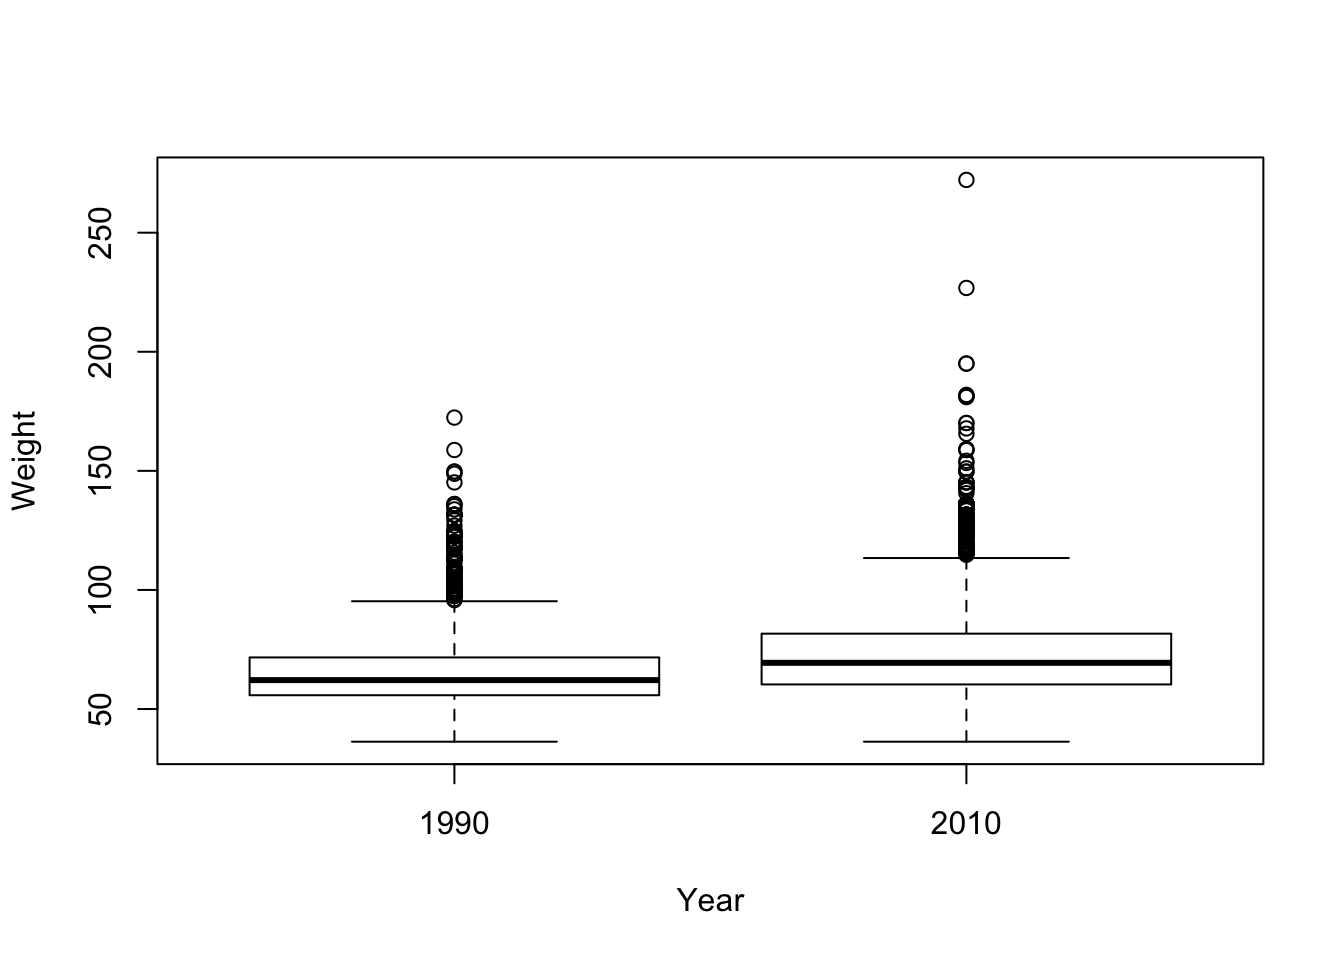
\includegraphics{_main_files/figure-latex/unnamed-chunk-24-1.pdf}

Statistical test

\begin{Shaded}
\begin{Highlighting}[]
\KeywordTok{t.test}\NormalTok{(Weight }\OperatorTok{~}\StringTok{ }\NormalTok{Year, brfssFemale)}
\end{Highlighting}
\end{Shaded}

\begin{verbatim}
## 
##  Welch Two Sample t-test
## 
## data:  Weight by Year
## t = -27.133, df = 11079, p-value < 2.2e-16
## alternative hypothesis: true difference in means is not equal to 0
## 95 percent confidence interval:
##  -8.723607 -7.548102
## sample estimates:
## mean in group 1990 mean in group 2010 
##           64.81838           72.95424
\end{verbatim}

\subsection{Weight and height in 2010
Males}\label{weight-and-height-in-2010-males}

Create a subset of the data

\begin{Shaded}
\begin{Highlighting}[]
\NormalTok{brfss2010Male <-}\StringTok{ }\KeywordTok{subset}\NormalTok{(brfss,  Year }\OperatorTok{==}\StringTok{ }\DecValTok{2010} \OperatorTok{&}\StringTok{ }\NormalTok{Sex }\OperatorTok{==}\StringTok{ "Male"}\NormalTok{)}
\KeywordTok{summary}\NormalTok{(brfss2010Male)}
\end{Highlighting}
\end{Shaded}

\begin{verbatim}
##       Age            Weight           Sex           Height      Year     
##  Min.   :18.00   Min.   : 36.29   Female:   0   Min.   :135   1990:   0  
##  1st Qu.:45.00   1st Qu.: 77.11   Male  :3679   1st Qu.:173   2010:3679  
##  Median :57.00   Median : 86.18                 Median :178              
##  Mean   :56.25   Mean   : 88.85                 Mean   :178              
##  3rd Qu.:68.00   3rd Qu.: 99.79                 3rd Qu.:183              
##  Max.   :99.00   Max.   :278.96                 Max.   :218              
##  NA's   :30      NA's   :49                     NA's   :31
\end{verbatim}

Visualize the relationship

\begin{Shaded}
\begin{Highlighting}[]
\KeywordTok{hist}\NormalTok{(brfss2010Male}\OperatorTok{$}\NormalTok{Weight)}
\end{Highlighting}
\end{Shaded}

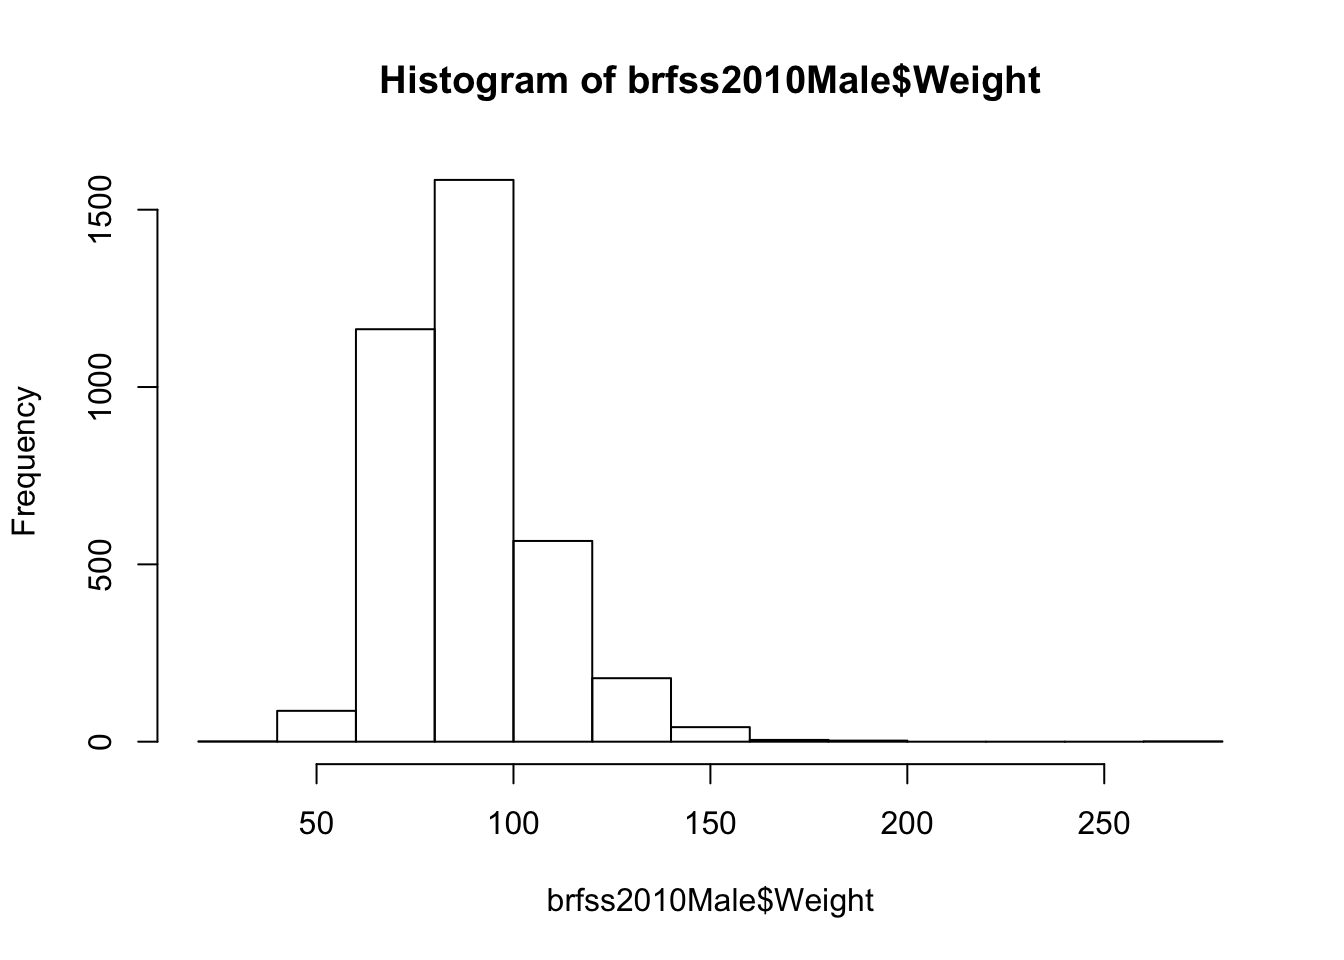
\includegraphics{_main_files/figure-latex/unnamed-chunk-27-1.pdf}

\begin{Shaded}
\begin{Highlighting}[]
\KeywordTok{hist}\NormalTok{(brfss2010Male}\OperatorTok{$}\NormalTok{Height)}
\end{Highlighting}
\end{Shaded}

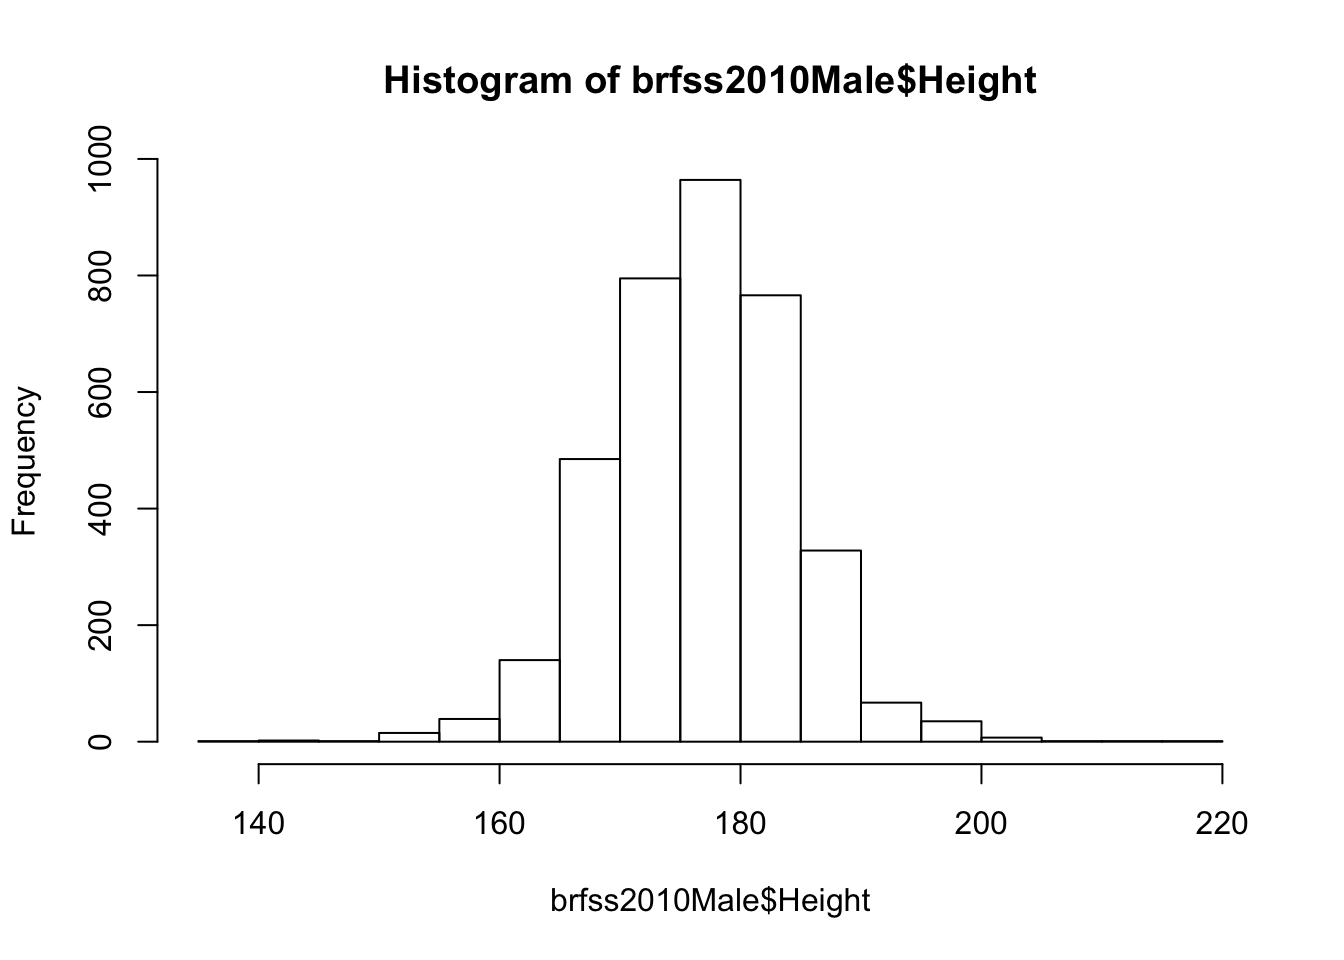
\includegraphics{_main_files/figure-latex/unnamed-chunk-27-2.pdf}

\begin{Shaded}
\begin{Highlighting}[]
\KeywordTok{plot}\NormalTok{(Weight }\OperatorTok{~}\StringTok{ }\NormalTok{Height, brfss2010Male)}
\end{Highlighting}
\end{Shaded}

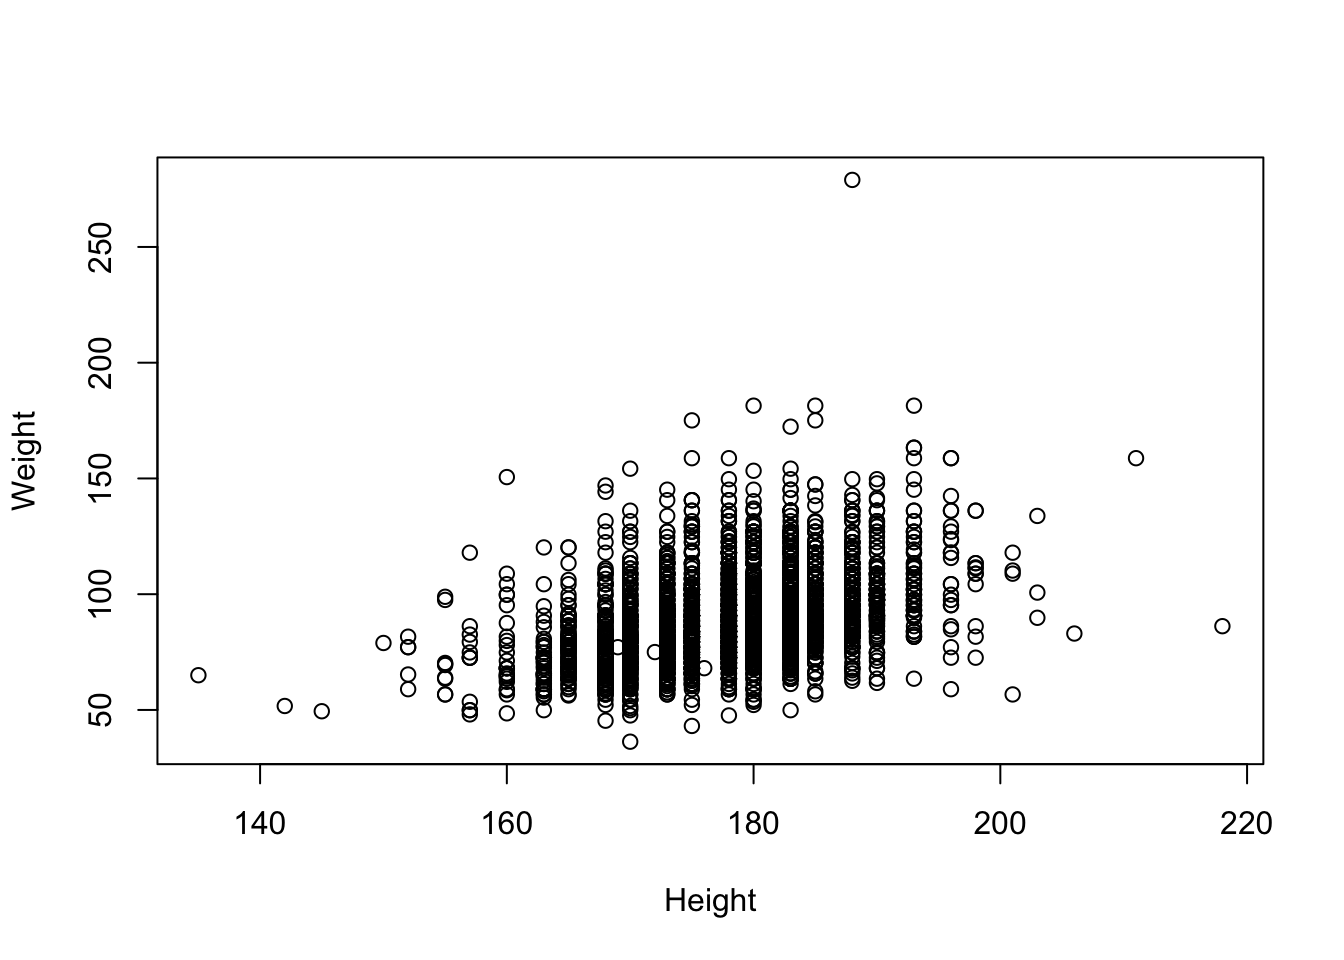
\includegraphics{_main_files/figure-latex/unnamed-chunk-27-3.pdf}

Fit a linear model (regression)

\begin{Shaded}
\begin{Highlighting}[]
\NormalTok{fit <-}\StringTok{ }\KeywordTok{lm}\NormalTok{(Weight }\OperatorTok{~}\StringTok{ }\NormalTok{Height, brfss2010Male)}
\NormalTok{fit}
\end{Highlighting}
\end{Shaded}

\begin{verbatim}
## 
## Call:
## lm(formula = Weight ~ Height, data = brfss2010Male)
## 
## Coefficients:
## (Intercept)       Height  
##    -86.8747       0.9873
\end{verbatim}

Summarize as ANOVA table

\begin{Shaded}
\begin{Highlighting}[]
\KeywordTok{anova}\NormalTok{(fit)}
\end{Highlighting}
\end{Shaded}

\begin{verbatim}
## Analysis of Variance Table
## 
## Response: Weight
##             Df  Sum Sq Mean Sq F value    Pr(>F)    
## Height       1  197664  197664   693.8 < 2.2e-16 ***
## Residuals 3617 1030484     285                      
## ---
## Signif. codes:  0 '***' 0.001 '**' 0.01 '*' 0.05 '.' 0.1 ' ' 1
\end{verbatim}

Plot points, superpose fitted regression line; where am I?

\begin{Shaded}
\begin{Highlighting}[]
\KeywordTok{plot}\NormalTok{(Weight }\OperatorTok{~}\StringTok{ }\NormalTok{Height, brfss2010Male)}
\KeywordTok{abline}\NormalTok{(fit, }\DataTypeTok{col=}\StringTok{"blue"}\NormalTok{, }\DataTypeTok{lwd=}\DecValTok{2}\NormalTok{)}
\KeywordTok{points}\NormalTok{(}\DecValTok{180}\NormalTok{, }\DecValTok{88}\NormalTok{, }\DataTypeTok{col=}\StringTok{"red"}\NormalTok{, }\DataTypeTok{cex=}\DecValTok{4}\NormalTok{, }\DataTypeTok{pch=}\DecValTok{20}\NormalTok{)}
\end{Highlighting}
\end{Shaded}

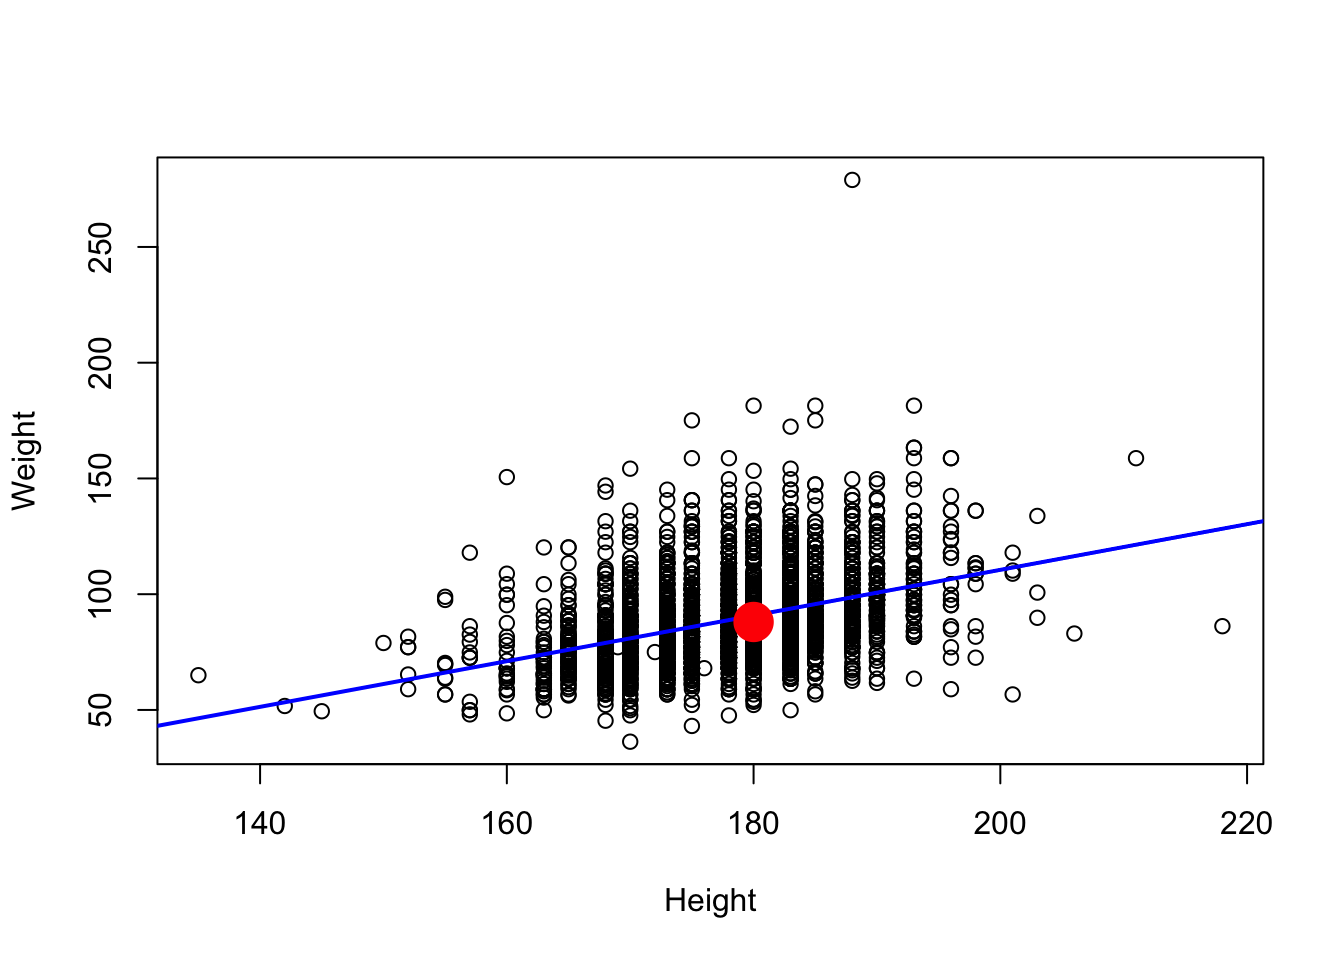
\includegraphics{_main_files/figure-latex/unnamed-chunk-30-1.pdf}

Class and available `methods'

\begin{Shaded}
\begin{Highlighting}[]
\KeywordTok{class}\NormalTok{(fit)                 }\CommentTok{# 'noun'}
\KeywordTok{methods}\NormalTok{(}\DataTypeTok{class=}\KeywordTok{class}\NormalTok{(fit))  }\CommentTok{# 'verb'}
\end{Highlighting}
\end{Shaded}

Diagnostics

\begin{Shaded}
\begin{Highlighting}[]
\KeywordTok{plot}\NormalTok{(fit)}
\NormalTok{?plot.lm}
\end{Highlighting}
\end{Shaded}

\section{Multivariate analysis}\label{multivariate-analysis}

This is a classic microarray experiment. Microarrays consist of
`probesets' that interogate genes for their level of expression. In the
experiment we're looking at, there are 12625 probesets measured on each
of the 128 samples. The raw expression levels estimated by microarray
assays require considerable pre-processing, the data we'll work with has
been pre-processed.

\subsection{Input and setup}\label{input-and-setup}

Start by finding the expression data file on disk.

\begin{Shaded}
\begin{Highlighting}[]
\NormalTok{path <-}\StringTok{ }\KeywordTok{file.choose}\NormalTok{()          }\CommentTok{# look for ALL-expression.csv}
\KeywordTok{stopifnot}\NormalTok{(}\KeywordTok{file.exists}\NormalTok{(path))}
\end{Highlighting}
\end{Shaded}

The data is stored in `comma-separate value' format, with each probeset
occupying a line, and the expression value for each sample in that
probeset separated by a comma. Input the data using \texttt{read.csv()}.
There are three challenges:

\begin{enumerate}
\def\labelenumi{\arabic{enumi}.}
\tightlist
\item
  The row names are present in the first column of the data. Tell
  \emph{R} this by adding the argument \texttt{row.names=1} to
  \texttt{read.csv()}.
\item
  By default, \emph{R} checks that column names do not look like
  numbers, but our column names \emph{do} look like numbers. Use the
  argument \texttt{check.colnames=FALSE} to over-ride \emph{R}'s
  default.
\item
  \texttt{read.csv()} returns a \texttt{data.frame}. We could use a
  \texttt{data.frame} to work with our data, but really it is a
  \texttt{matrix()} -- the columns are of the same type and measure the
  same thing. Use \texttt{as.matrix()} to coerce the \texttt{data.frame}
  we input to a \texttt{matrix}.
\end{enumerate}

\begin{Shaded}
\begin{Highlighting}[]
\NormalTok{exprs <-}\StringTok{ }\KeywordTok{read.csv}\NormalTok{(path, }\DataTypeTok{row.names=}\DecValTok{1}\NormalTok{, }\DataTypeTok{check.names=}\OtherTok{FALSE}\NormalTok{)}
\NormalTok{exprs <-}\StringTok{ }\KeywordTok{as.matrix}\NormalTok{(exprs)}
\KeywordTok{class}\NormalTok{(exprs)}
\end{Highlighting}
\end{Shaded}

\begin{verbatim}
## [1] "matrix"
\end{verbatim}

\begin{Shaded}
\begin{Highlighting}[]
\KeywordTok{dim}\NormalTok{(exprs)}
\end{Highlighting}
\end{Shaded}

\begin{verbatim}
## [1] 12625   128
\end{verbatim}

\begin{Shaded}
\begin{Highlighting}[]
\NormalTok{exprs[}\DecValTok{1}\OperatorTok{:}\DecValTok{6}\NormalTok{, }\DecValTok{1}\OperatorTok{:}\DecValTok{10}\NormalTok{]}
\end{Highlighting}
\end{Shaded}

\begin{verbatim}
##              01005     01010    03002    04006    04007     04008
## 1000_at   7.597323  7.479445 7.567593 7.384684 7.905312  7.065914
## 1001_at   5.046194  4.932537 4.799294 4.922627 4.844565  5.147762
## 1002_f_at 3.900466  4.208155 3.886169 4.206798 3.416923  3.945869
## 1003_s_at 5.903856  6.169024 5.860459 6.116890 5.687997  6.208061
## 1004_at   5.925260  5.912780 5.893209 6.170245 5.615210  5.923487
## 1005_at   8.570990 10.428299 9.616713 9.937155 9.983809 10.063484
##               04010     04016    06002     08001
## 1000_at    7.474537  7.536119 7.183331  7.735545
## 1001_at    5.122518  5.016132 5.288943  4.633217
## 1002_f_at  4.150506  3.576360 3.900935  3.630190
## 1003_s_at  6.292713  5.665991 5.842326  5.875375
## 1004_at    6.046607  5.738218 5.994515  5.748350
## 1005_at   10.662059 11.269115 8.812869 10.165159
\end{verbatim}

\begin{Shaded}
\begin{Highlighting}[]
\KeywordTok{range}\NormalTok{(exprs)}
\end{Highlighting}
\end{Shaded}

\begin{verbatim}
## [1]  1.984919 14.126571
\end{verbatim}

We'll make use of the data describing the samples

\begin{Shaded}
\begin{Highlighting}[]
\NormalTok{path <-}\StringTok{ }\KeywordTok{file.choose}\NormalTok{()         }\CommentTok{# look for ALL-phenoData.csv}
\KeywordTok{stopifnot}\NormalTok{(}\KeywordTok{file.exists}\NormalTok{(path))}
\end{Highlighting}
\end{Shaded}

\begin{Shaded}
\begin{Highlighting}[]
\NormalTok{pdata <-}\StringTok{ }\KeywordTok{read.csv}\NormalTok{(path, }\DataTypeTok{row.names=}\DecValTok{1}\NormalTok{)}
\KeywordTok{class}\NormalTok{(pdata)}
\end{Highlighting}
\end{Shaded}

\begin{verbatim}
## [1] "data.frame"
\end{verbatim}

\begin{Shaded}
\begin{Highlighting}[]
\KeywordTok{dim}\NormalTok{(pdata)}
\end{Highlighting}
\end{Shaded}

\begin{verbatim}
## [1] 128  21
\end{verbatim}

\begin{Shaded}
\begin{Highlighting}[]
\KeywordTok{head}\NormalTok{(pdata)}
\end{Highlighting}
\end{Shaded}

\begin{verbatim}
##        cod diagnosis sex age BT remission CR   date.cr t.4.11. t.9.22.
## 01005 1005 5/21/1997   M  53 B2        CR CR  8/6/1997   FALSE    TRUE
## 01010 1010 3/29/2000   M  19 B2        CR CR 6/27/2000   FALSE   FALSE
## 03002 3002 6/24/1998   F  52 B4        CR CR 8/17/1998      NA      NA
## 04006 4006 7/17/1997   M  38 B1        CR CR  9/8/1997    TRUE   FALSE
## 04007 4007 7/22/1997   M  57 B2        CR CR 9/17/1997   FALSE   FALSE
## 04008 4008 7/30/1997   M  17 B1        CR CR 9/27/1997   FALSE   FALSE
##       cyto.normal        citog mol.biol fusion.protein mdr   kinet   ccr
## 01005       FALSE      t(9;22)  BCR/ABL           p210 NEG dyploid FALSE
## 01010       FALSE  simple alt.      NEG           <NA> POS dyploid FALSE
## 03002          NA         <NA>  BCR/ABL           p190 NEG dyploid FALSE
## 04006       FALSE      t(4;11) ALL1/AF4           <NA> NEG dyploid FALSE
## 04007       FALSE      del(6q)      NEG           <NA> NEG dyploid FALSE
## 04008       FALSE complex alt.      NEG           <NA> NEG hyperd. FALSE
##       relapse transplant               f.u date.last.seen
## 01005   FALSE       TRUE BMT / DEATH IN CR           <NA>
## 01010    TRUE      FALSE               REL      8/28/2000
## 03002    TRUE      FALSE               REL     10/15/1999
## 04006    TRUE      FALSE               REL      1/23/1998
## 04007    TRUE      FALSE               REL      11/4/1997
## 04008    TRUE      FALSE               REL     12/15/1997
\end{verbatim}

Some of the results below involve plots, and it's convenient to choose
pretty and functional colors. We use the
\href{https://cran.r-project.org/?package=RColorBrewer}{RColorBrewer}
package; see \href{http://colorbrewer.org}{colorbrewer.org}

\begin{Shaded}
\begin{Highlighting}[]
\KeywordTok{library}\NormalTok{(RColorBrewer)  ## not available? install package via RStudio}
\NormalTok{highlight <-}\StringTok{ }\KeywordTok{brewer.pal}\NormalTok{(}\DecValTok{3}\NormalTok{, }\StringTok{"Set2"}\NormalTok{)[}\DecValTok{1}\OperatorTok{:}\DecValTok{2}\NormalTok{]}
\end{Highlighting}
\end{Shaded}

`highlight' is a vector of length 2, light and dark green.

For more options see \texttt{?RColorBrewer} and to view the predefined
palettes \texttt{display.brewer.all()}

\subsection{Cleaning}\label{cleaning}

We'll add a column to \texttt{pdata}, derived from the \texttt{BT}
column, to indicate whether the sample is B-cell or T-cell ALL.

\begin{Shaded}
\begin{Highlighting}[]
\NormalTok{pdata}\OperatorTok{$}\NormalTok{BorT <-}\StringTok{ }\KeywordTok{factor}\NormalTok{(}\KeywordTok{substr}\NormalTok{(pdata}\OperatorTok{$}\NormalTok{BT, }\DecValTok{1}\NormalTok{, }\DecValTok{1}\NormalTok{))}
\end{Highlighting}
\end{Shaded}

Microarray expression data is usually represented as a matrix of genes
as rows and samples as columns. Statisticians usually think of their
data as samples as rows, features as columns. So we'll transpose the
expression values

\begin{Shaded}
\begin{Highlighting}[]
\NormalTok{exprs <-}\StringTok{ }\KeywordTok{t}\NormalTok{(exprs)}
\end{Highlighting}
\end{Shaded}

Confirm that the \texttt{pdata} rows correspond to the \texttt{exprs}
rows.

\begin{Shaded}
\begin{Highlighting}[]
\KeywordTok{stopifnot}\NormalTok{(}\KeywordTok{identical}\NormalTok{(}\KeywordTok{rownames}\NormalTok{(pdata), }\KeywordTok{rownames}\NormalTok{(exprs)))}
\end{Highlighting}
\end{Shaded}

\subsection{Unsupervised machine learning -- multi-dimensional
scaling}\label{unsupervised-machine-learning-multi-dimensional-scaling}

Reduce high-dimensional data to lower dimension for visualization.

Calculate distance between \emph{samples} (requires that the expression
matrix be transposed).

\begin{Shaded}
\begin{Highlighting}[]
\NormalTok{d <-}\StringTok{ }\KeywordTok{dist}\NormalTok{(exprs)}
\end{Highlighting}
\end{Shaded}

Use the \texttt{cmdscale()} function to summarize the distance matrix
into two points in two dimensions.

\begin{Shaded}
\begin{Highlighting}[]
\NormalTok{cmd <-}\StringTok{ }\KeywordTok{cmdscale}\NormalTok{(d)}
\end{Highlighting}
\end{Shaded}

Visualize the result, coloring points by B- or T-cell status

\begin{Shaded}
\begin{Highlighting}[]
\KeywordTok{plot}\NormalTok{(cmd, }\DataTypeTok{col=}\NormalTok{highlight[pdata}\OperatorTok{$}\NormalTok{BorT])}
\end{Highlighting}
\end{Shaded}

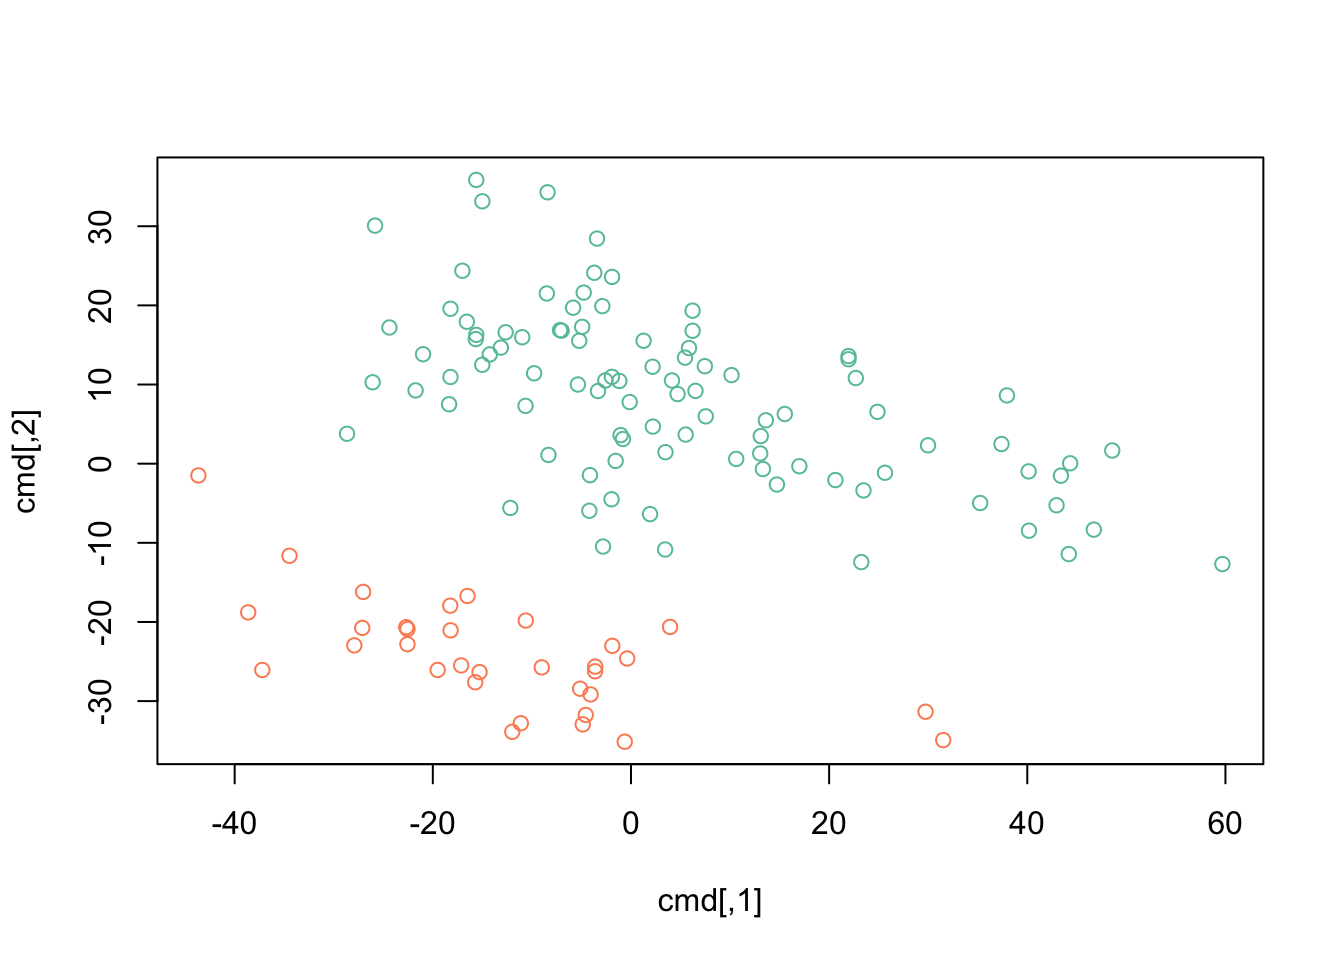
\includegraphics{_main_files/figure-latex/unnamed-chunk-43-1.pdf}

\section{\texorpdfstring{Using \emph{R} in real
life}{Using R in real life}}\label{using-r-in-real-life}

\subsection{Organizing work}\label{organizing-work}

Usually, work is organized into a directory with:

\begin{itemize}
\tightlist
\item
  A folder containing \emph{R} scripts
  (\texttt{scripts/BRFSS-visualize.R})
\item
  `External' data like the csv files that we've been working with,
  usually in a separate folder (\texttt{extdata/BRFSS-subset.csv})
\item
  (sometimes) \emph{R} objects written to disk using \texttt{saveRDS()}
  (\texttt{.rds} files) that represent final results or intermediate
  `checkpoints' (\texttt{extdata/ALL-cleaned.rds}). Read the data into
  an \emph{R} session using \texttt{readRDS()}.
\item
  Use \texttt{setwd()} to navigate to folder containing scripts/,
  extdata/ folder
\item
  Source an entire script with
  \texttt{source("scripts/BRFSS-visualization.R")}.
\end{itemize}

\emph{R} can also save the state of the current session (prompt when
choosing to \texttt{quit()} \emph{R}), and to view and save the
\texttt{history()} of the the current session; I do not find these to be
helpful in my own work flows.

\subsection{\texorpdfstring{\emph{R}
Packages}{R Packages}}\label{r-packages}

All the functionality we have been using comes from \emph{packages} that
are automatically \emph{loaded} when \emph{R} starts. Loaded packages
are on the \texttt{search()} path.

\begin{Shaded}
\begin{Highlighting}[]
\KeywordTok{search}\NormalTok{()}
\end{Highlighting}
\end{Shaded}

\begin{verbatim}
##  [1] ".GlobalEnv"           "package:RColorBrewer" "package:stats"       
##  [4] "package:graphics"     "package:grDevices"    "package:utils"       
##  [7] "package:datasets"     "package:methods"      "Autoloads"           
## [10] "package:base"
\end{verbatim}

Additional packages may be \emph{installed} in \emph{R}'s libraries. Use
`installed.packages() or the \emph{RStudio} interface to see installed
packages. To use these packages, it is necessary to attach them to the
search path, e.g., for survival analysis

\begin{Shaded}
\begin{Highlighting}[]
\KeywordTok{library}\NormalTok{(}\StringTok{"survival"}\NormalTok{)}
\end{Highlighting}
\end{Shaded}

There are many thousands of \emph{R} packages, and not all of them are
installed in a single installation. Important repositories are

\begin{itemize}
\tightlist
\item
  CRAN: \url{https://cran.r-project.org/}
\item
  Bioconductor: \url{https://bioconductor.org/packages}
\end{itemize}

Packages can be discovered in various ways, including
\href{https://cran.r-project.org/web/views/}{CRAN Task Views} and the
\href{https://bioconductor.org}{\emph{Bioconductor} web} and
\href{https://support.bioconductor.org}{\emph{Bioconductor} support}
sites.

To install a package, use \texttt{install.packages()} or, for
\emph{Bioconductor} packages, instructions on the package landing page,
e.g., for
\href{https://bioconductor.org/packages/GenomicRanges}{GenomicRanges}.
Here we install the
\href{https://cran.r-project.org/package=ggplot2}{ggplot2} package.

\begin{Shaded}
\begin{Highlighting}[]
\KeywordTok{install.packages}\NormalTok{(}\StringTok{"ggplot2"}\NormalTok{, }\DataTypeTok{repos=}\StringTok{"https://cran.r-project.org"}\NormalTok{)}
\end{Highlighting}
\end{Shaded}

A package needs to be installed once, and then can be used in any
\emph{R} session.

\section{Graphics and Visualization}\label{graphics-and-visualization}

Load the BRFSS-subset.csv data

\begin{Shaded}
\begin{Highlighting}[]
\NormalTok{path <-}\StringTok{ "BRFSS-subset.csv"}   \CommentTok{# or file.choose()}
\NormalTok{brfss <-}\StringTok{ }\KeywordTok{read.csv}\NormalTok{(path)}
\end{Highlighting}
\end{Shaded}

Clean it by coercing \texttt{Year} to factor

\begin{Shaded}
\begin{Highlighting}[]
\NormalTok{brfss}\OperatorTok{$}\NormalTok{Year <-}\StringTok{ }\KeywordTok{factor}\NormalTok{(brfss}\OperatorTok{$}\NormalTok{Year)}
\end{Highlighting}
\end{Shaded}

\subsection{\texorpdfstring{Base \emph{R}
Graphics}{Base R Graphics}}\label{base-r-graphics}

Useful for quick exploration during a normal work flow.

\begin{itemize}
\item
  Main functions: \texttt{plot()}, \texttt{hist()}, \texttt{boxplot()},
  \ldots{}
\item
  Graphical parameters -- see \texttt{?par}, but often provided as
  arguments to \texttt{plot()}, etc.
\item
  Construct complicated plots by layering information, e.g., points,
  regression line, annotation.

\begin{Shaded}
\begin{Highlighting}[]
\NormalTok{brfss2010Male <-}\StringTok{ }\KeywordTok{subset}\NormalTok{(brfss, (Year }\OperatorTok{==}\StringTok{ }\DecValTok{2010}\NormalTok{) }\OperatorTok{&}\StringTok{ }\NormalTok{(Sex }\OperatorTok{==}\StringTok{ "Male"}\NormalTok{))}
\NormalTok{fit <-}\StringTok{ }\KeywordTok{lm}\NormalTok{(Weight }\OperatorTok{~}\StringTok{ }\NormalTok{Height, brfss2010Male)}

\KeywordTok{plot}\NormalTok{(Weight }\OperatorTok{~}\StringTok{ }\NormalTok{Height, brfss2010Male, }\DataTypeTok{main=}\StringTok{"2010, Males"}\NormalTok{)}
\KeywordTok{abline}\NormalTok{(fit, }\DataTypeTok{lwd=}\DecValTok{2}\NormalTok{, }\DataTypeTok{col=}\StringTok{"blue"}\NormalTok{)}
\KeywordTok{points}\NormalTok{(}\DecValTok{180}\NormalTok{, }\DecValTok{90}\NormalTok{, }\DataTypeTok{pch=}\DecValTok{20}\NormalTok{, }\DataTypeTok{cex=}\DecValTok{3}\NormalTok{, }\DataTypeTok{col=}\StringTok{"red"}\NormalTok{)}
\end{Highlighting}
\end{Shaded}

  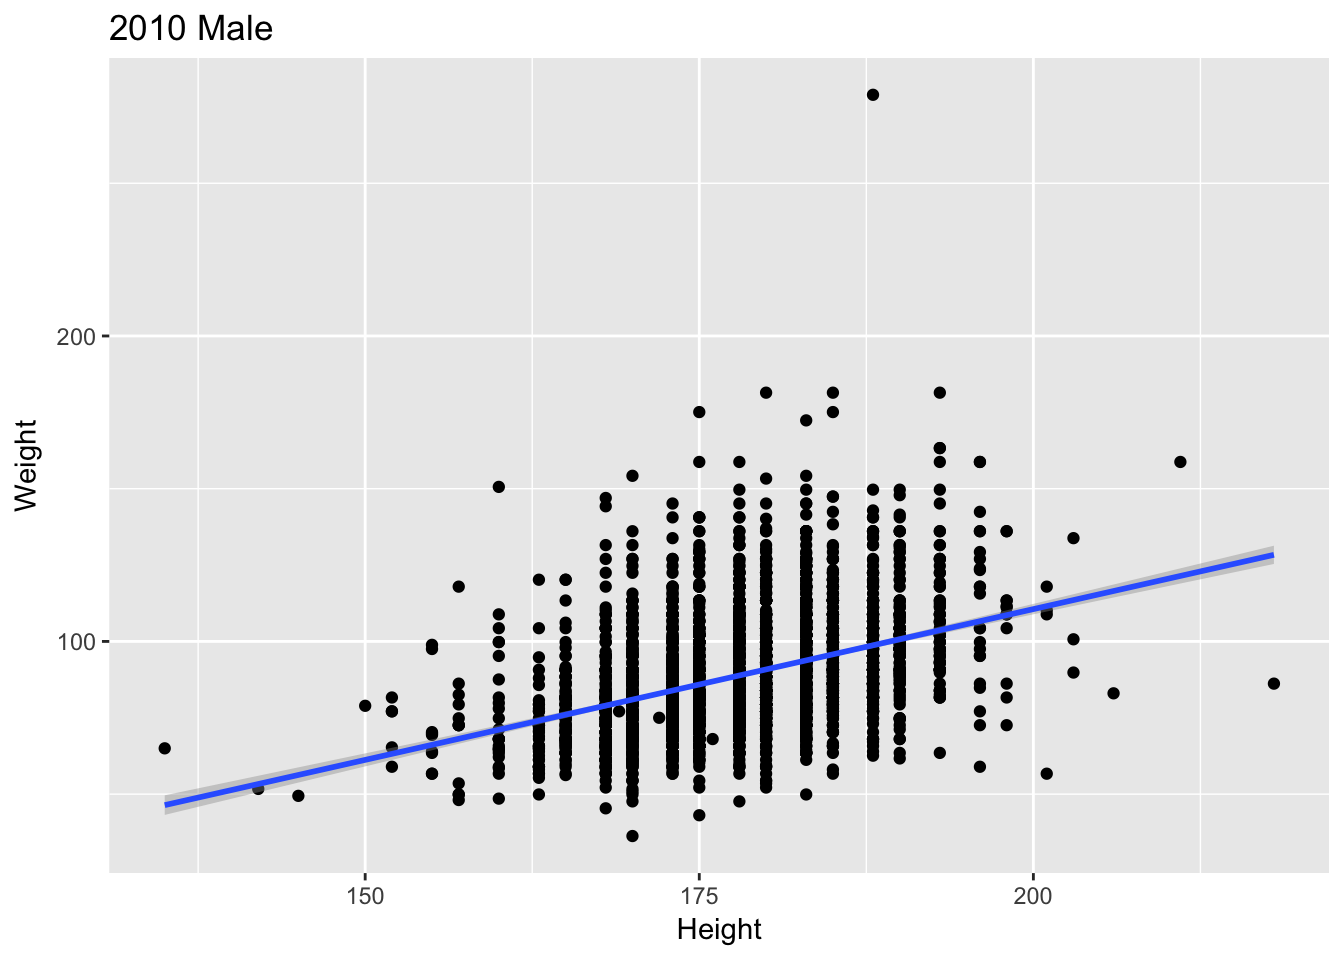
\includegraphics{_main_files/figure-latex/unnamed-chunk-49-1.pdf}
\item
  Approach to complicated graphics: create a grid of panels (e.g.,
  \texttt{par(mfrows=c(1,\ 2))}, populate with plots, restore original
  layout.

\begin{Shaded}
\begin{Highlighting}[]
\NormalTok{brfssFemale <-}\StringTok{ }\KeywordTok{subset}\NormalTok{(brfss, Sex}\OperatorTok{==}\StringTok{"Female"}\NormalTok{)}

\NormalTok{opar =}\StringTok{ }\KeywordTok{par}\NormalTok{(}\DataTypeTok{mfrow=}\KeywordTok{c}\NormalTok{(}\DecValTok{2}\NormalTok{, }\DecValTok{1}\NormalTok{))     }\CommentTok{# layout: 2 'rows' and 1 'column'}
\KeywordTok{hist}\NormalTok{(                         }\CommentTok{# first panel -- 1990}
\NormalTok{    brfssFemale[ brfssFemale}\OperatorTok{$}\NormalTok{Year }\OperatorTok{==}\StringTok{ }\DecValTok{1990}\NormalTok{, }\StringTok{"Weight"}\NormalTok{ ],}
    \DataTypeTok{main =} \StringTok{"Female, 1990"}\NormalTok{)}
\KeywordTok{hist}\NormalTok{(                         }\CommentTok{# second panel -- 2010}
\NormalTok{    brfssFemale[ brfssFemale}\OperatorTok{$}\NormalTok{Year }\OperatorTok{==}\StringTok{ }\DecValTok{2010}\NormalTok{, }\StringTok{"Weight"}\NormalTok{ ],}
    \DataTypeTok{main =} \StringTok{"Female, 2010"}\NormalTok{)}
\end{Highlighting}
\end{Shaded}

  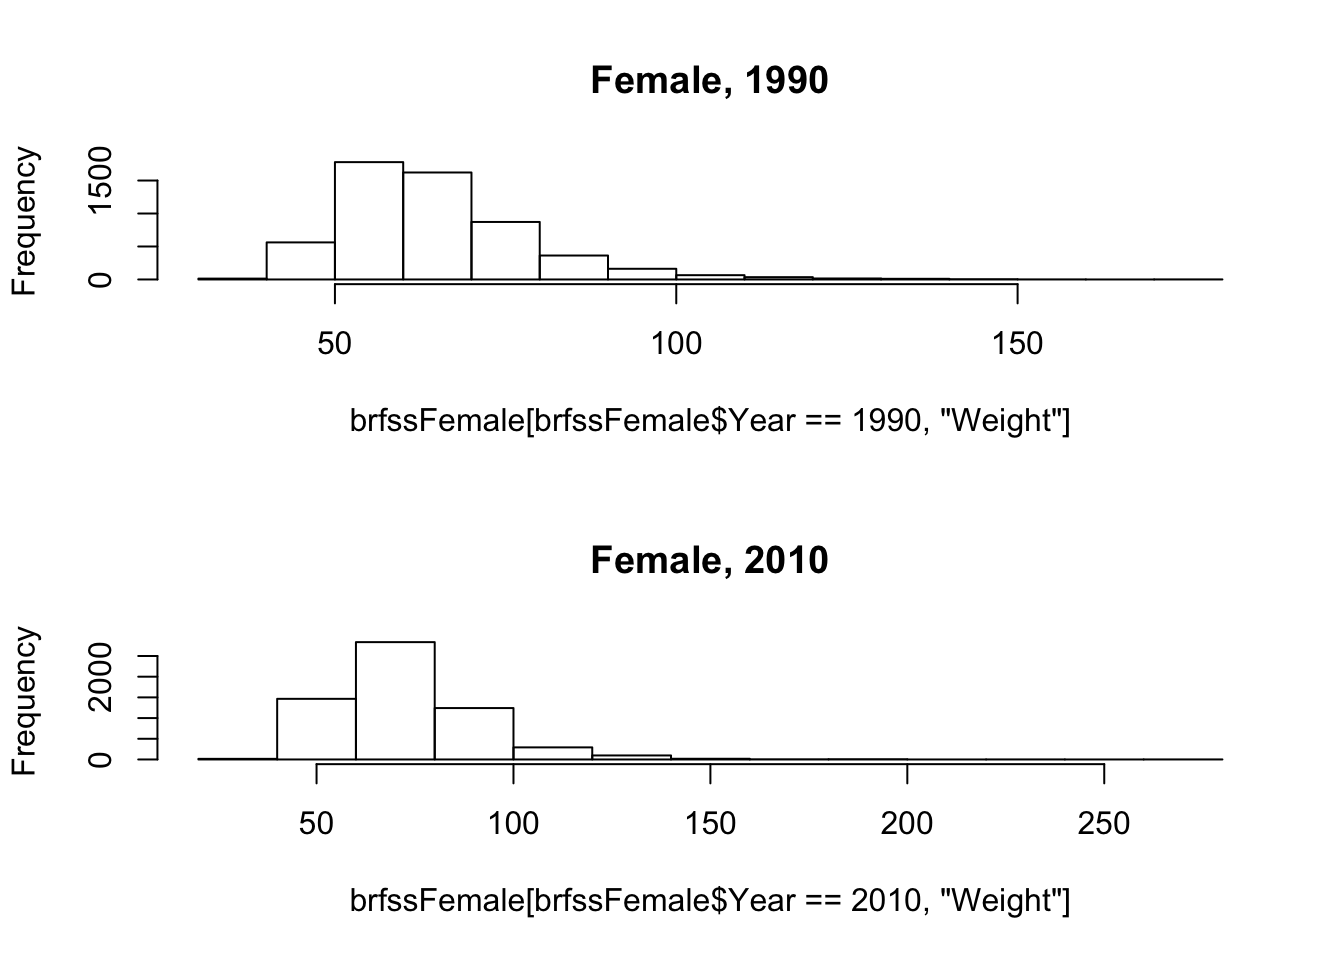
\includegraphics{_main_files/figure-latex/unnamed-chunk-50-1.pdf}

\begin{Shaded}
\begin{Highlighting}[]
\KeywordTok{par}\NormalTok{(opar)                      }\CommentTok{# restore original layout}
\end{Highlighting}
\end{Shaded}
\end{itemize}

\subsection{What makes for a good graphical
display?}\label{what-makes-for-a-good-graphical-display}

\begin{itemize}
\tightlist
\item
  Common scales for comparison
\item
  Efficient use of space
\item
  Careful color choice -- qualitative, gradient, divergent schemes;
  color blind aware; \ldots{}
\item
  Emphasis on data rather than labels
\item
  Convey statistical uncertainty
\end{itemize}

\subsection{Grammar of Graphics:
ggplot2}\label{grammar-of-graphics-ggplot2}

\begin{Shaded}
\begin{Highlighting}[]
\KeywordTok{library}\NormalTok{(ggplot2)}
\end{Highlighting}
\end{Shaded}

\begin{itemize}
\tightlist
\item
  \url{http://docs.ggplot2.org}
\end{itemize}

`Grammar of graphics'

\begin{itemize}
\item
  Specify data and `aesthetics' (\texttt{aes()}) to be plotted
\item
  Add layers (\texttt{geom\_*()}) of information

\begin{Shaded}
\begin{Highlighting}[]
\KeywordTok{ggplot}\NormalTok{(brfss2010Male, }\KeywordTok{aes}\NormalTok{(}\DataTypeTok{x=}\NormalTok{Height, }\DataTypeTok{y=}\NormalTok{Weight)) }\OperatorTok{+}
\StringTok{    }\KeywordTok{geom_point}\NormalTok{() }\OperatorTok{+}
\StringTok{    }\KeywordTok{geom_smooth}\NormalTok{(}\DataTypeTok{method=}\StringTok{"lm"}\NormalTok{)}
\end{Highlighting}
\end{Shaded}

  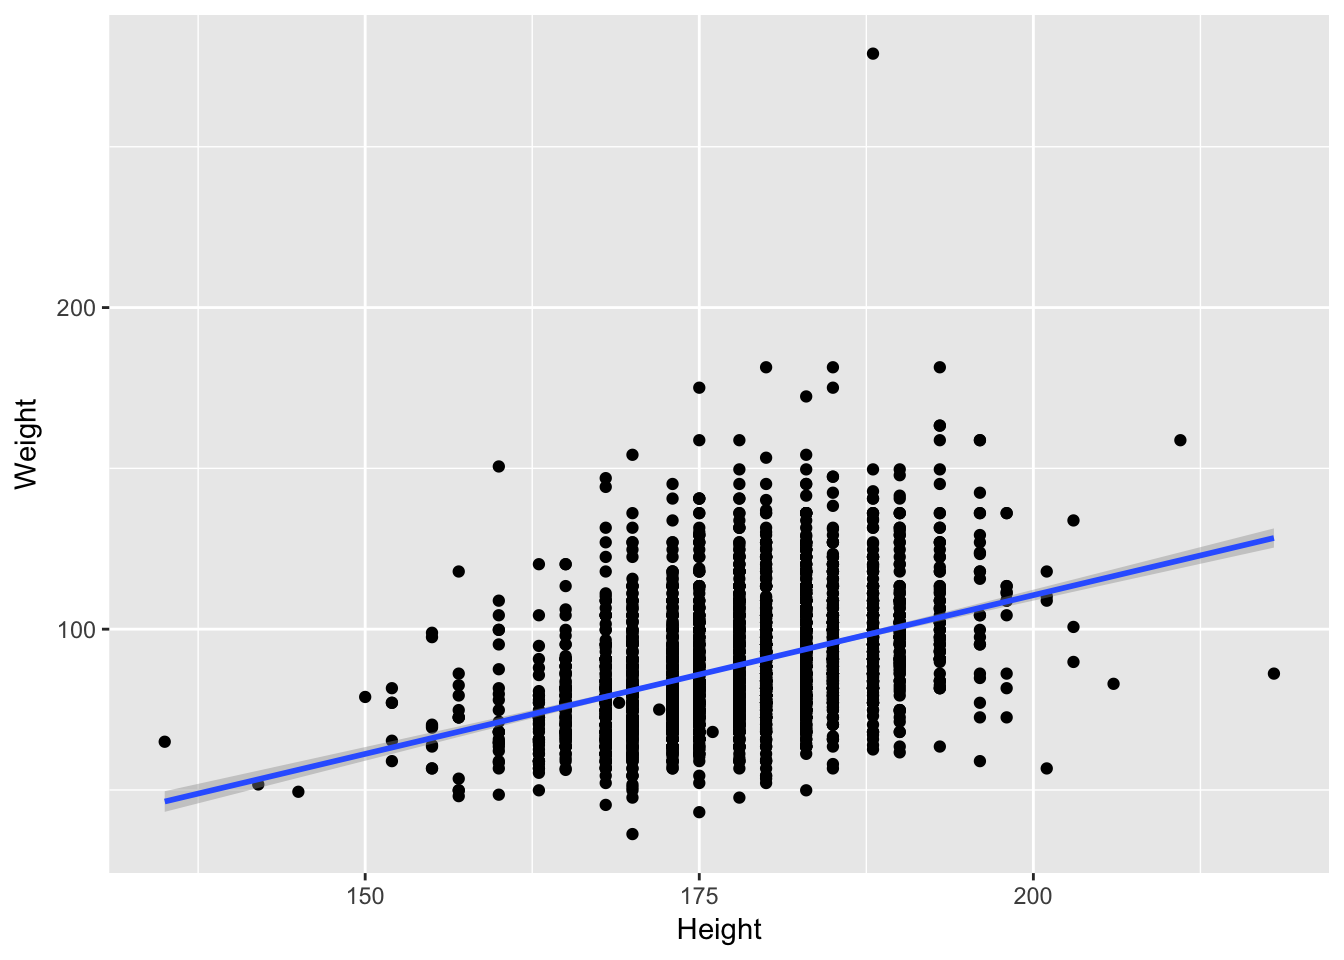
\includegraphics{_main_files/figure-latex/unnamed-chunk-52-1.pdf}
\item
  Capture a plot and augment it

\begin{Shaded}
\begin{Highlighting}[]
\NormalTok{plt <-}\StringTok{ }\KeywordTok{ggplot}\NormalTok{(brfss2010Male, }\KeywordTok{aes}\NormalTok{(}\DataTypeTok{x=}\NormalTok{Height, }\DataTypeTok{y=}\NormalTok{Weight)) }\OperatorTok{+}
\StringTok{    }\KeywordTok{geom_point}\NormalTok{() }\OperatorTok{+}
\StringTok{    }\KeywordTok{geom_smooth}\NormalTok{(}\DataTypeTok{method=}\StringTok{"lm"}\NormalTok{)}
\NormalTok{plt }\OperatorTok{+}\StringTok{ }\KeywordTok{labs}\NormalTok{(}\DataTypeTok{title =} \StringTok{"2010 Male"}\NormalTok{)}
\end{Highlighting}
\end{Shaded}

  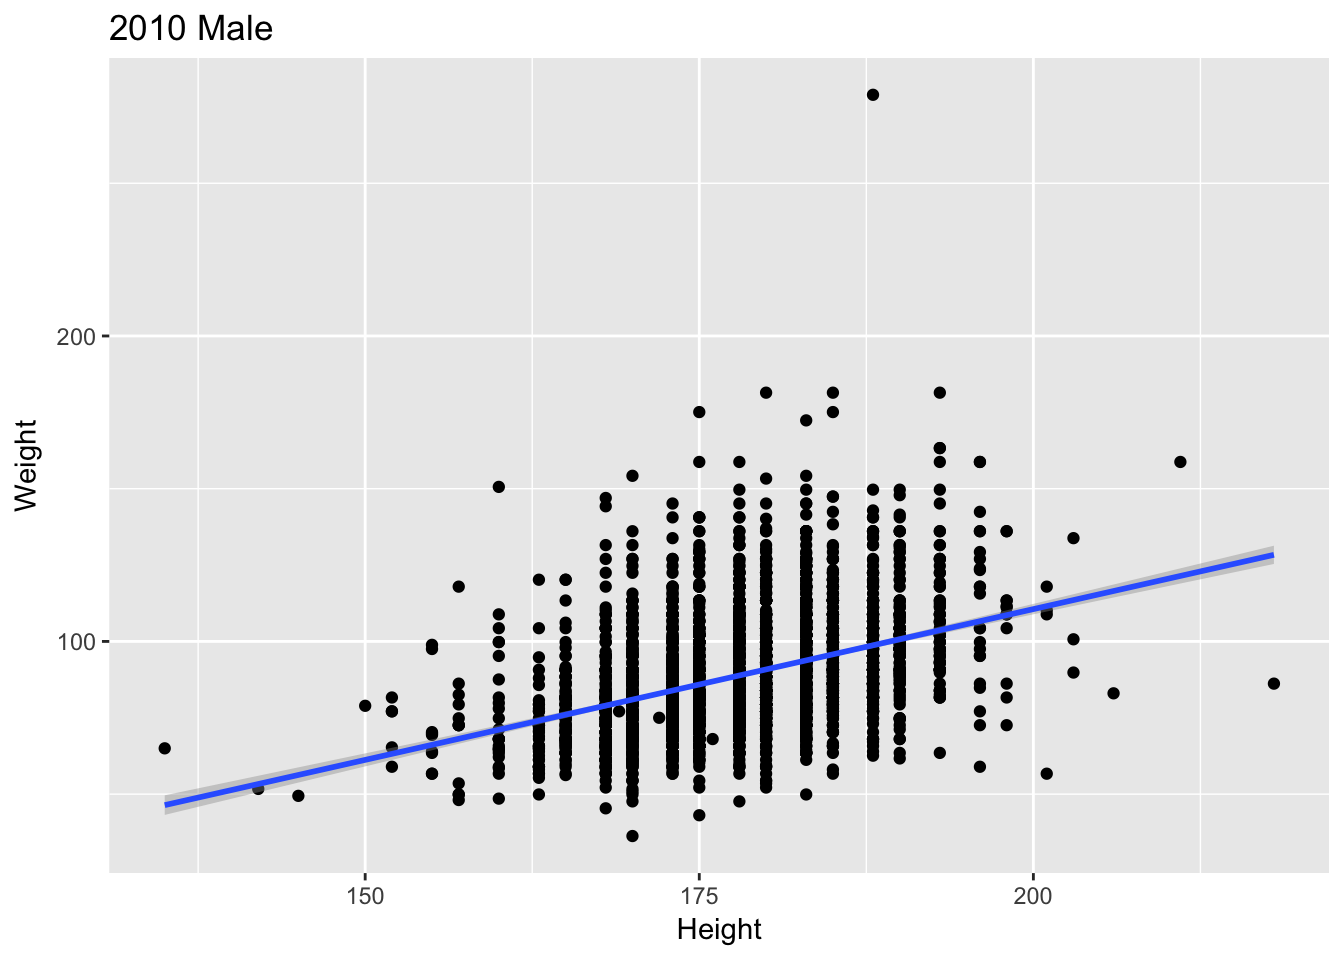
\includegraphics{_main_files/figure-latex/unnamed-chunk-53-1.pdf}
\item
  Use \texttt{facet\_*()} for layouts

\begin{Shaded}
\begin{Highlighting}[]
\KeywordTok{ggplot}\NormalTok{(brfssFemale, }\KeywordTok{aes}\NormalTok{(}\DataTypeTok{x=}\NormalTok{Height, }\DataTypeTok{y=}\NormalTok{Weight)) }\OperatorTok{+}
\StringTok{    }\KeywordTok{geom_point}\NormalTok{() }\OperatorTok{+}\StringTok{ }\KeywordTok{geom_smooth}\NormalTok{(}\DataTypeTok{method=}\StringTok{"lm"}\NormalTok{) }\OperatorTok{+}
\StringTok{    }\KeywordTok{facet_grid}\NormalTok{(. }\OperatorTok{~}\StringTok{ }\NormalTok{Year)}
\end{Highlighting}
\end{Shaded}

  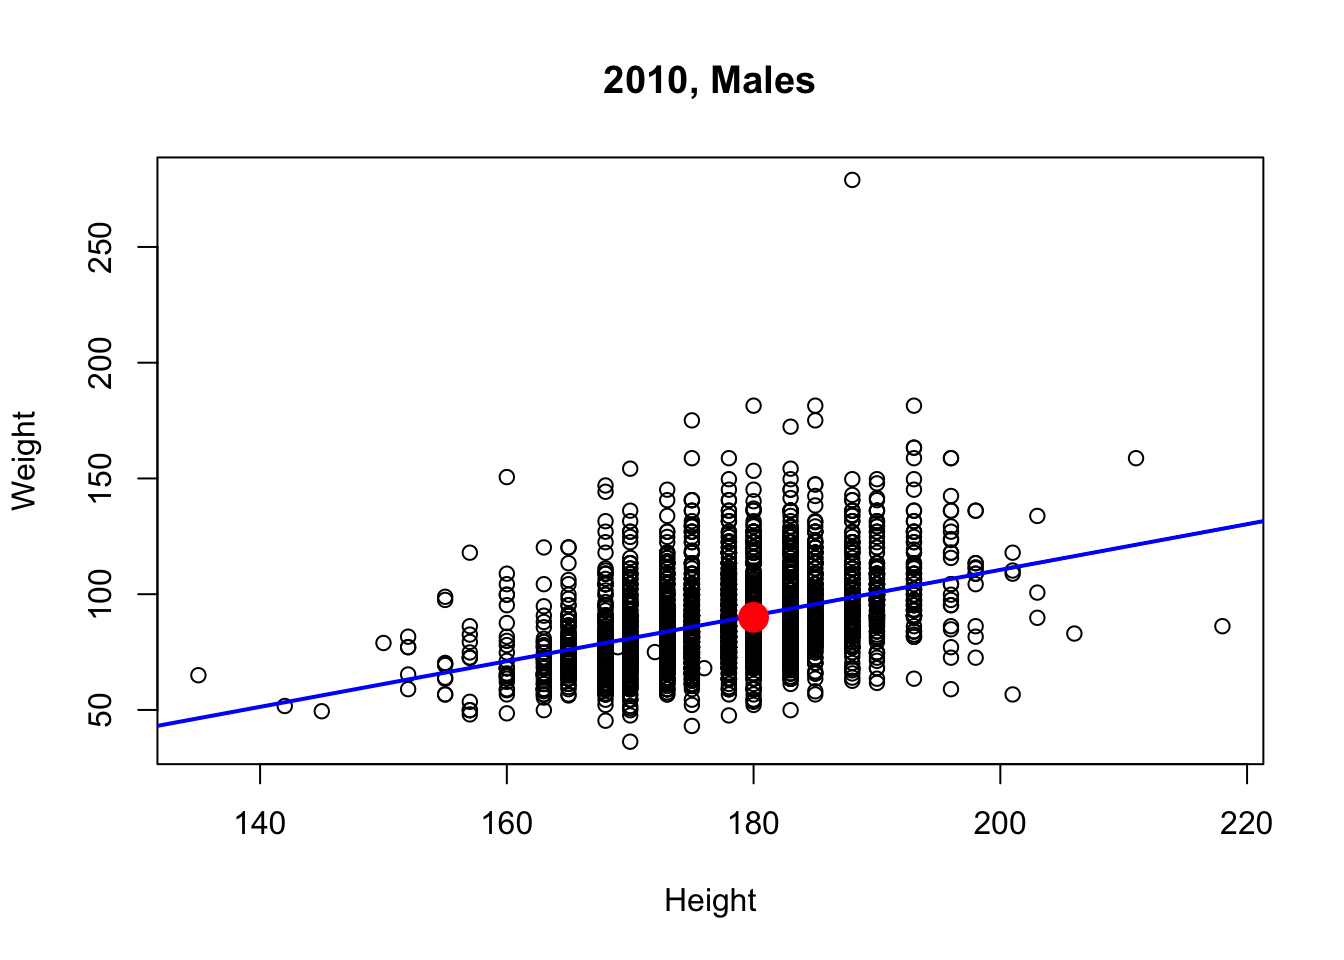
\includegraphics{_main_files/figure-latex/unnamed-chunk-54-1.pdf}
\item
  Choose display to emphasize relevant aspects of data

\begin{Shaded}
\begin{Highlighting}[]
\KeywordTok{ggplot}\NormalTok{(brfssFemale, }\KeywordTok{aes}\NormalTok{(Weight, }\DataTypeTok{fill=}\NormalTok{Year)) }\OperatorTok{+}
\StringTok{    }\KeywordTok{geom_density}\NormalTok{(}\DataTypeTok{alpha=}\NormalTok{.}\DecValTok{2}\NormalTok{)}
\end{Highlighting}
\end{Shaded}

  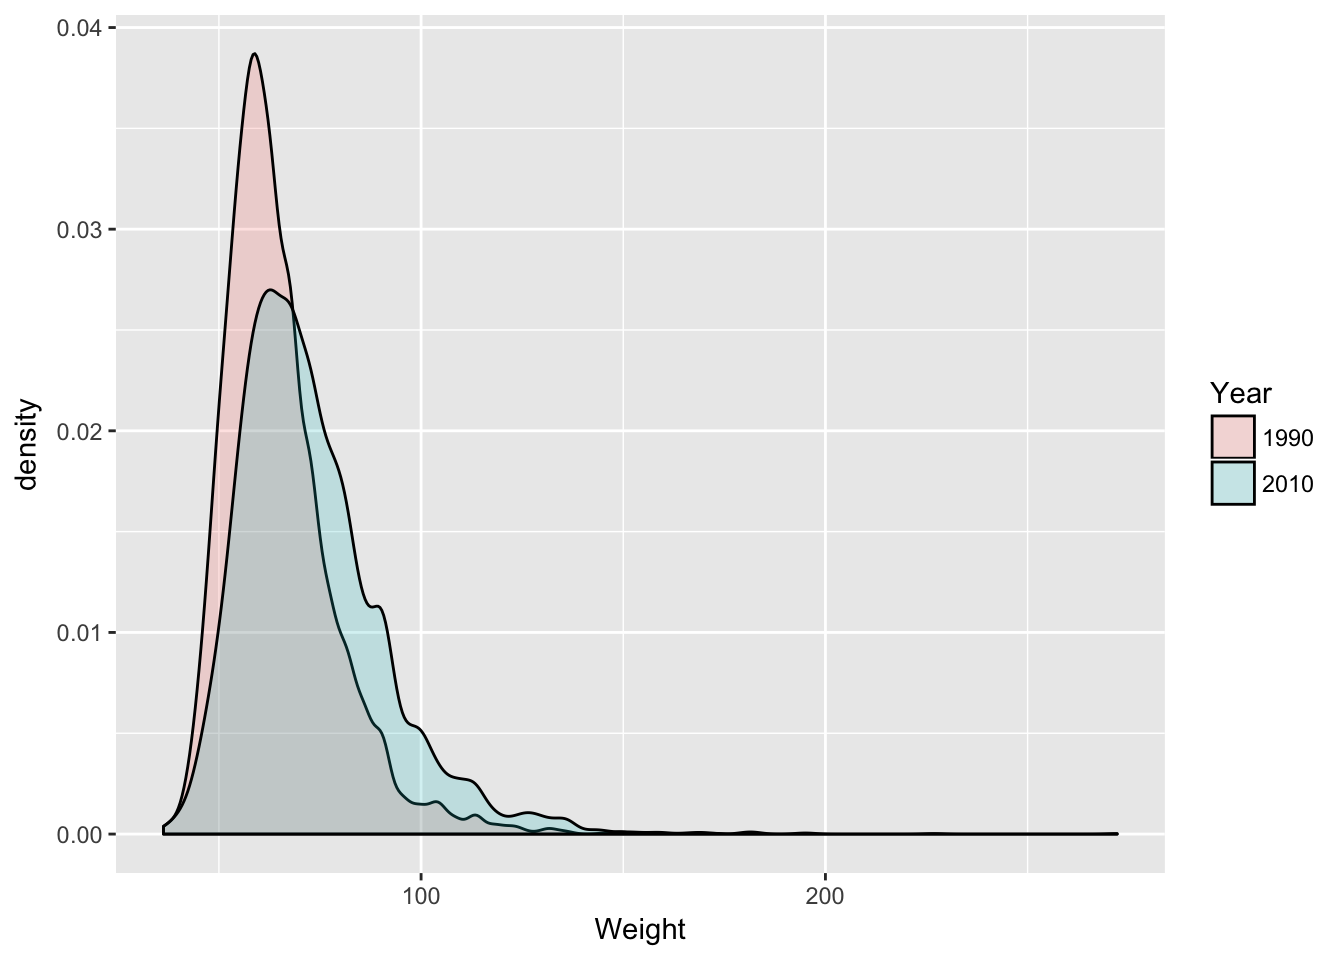
\includegraphics{_main_files/figure-latex/unnamed-chunk-55-1.pdf}
\end{itemize}


\end{document}
